%Version 3.1 December 2024
% See section 11 of the User Manual for version history
%
%%%%%%%%%%%%%%%%%%%%%%%%%%%%%%%%%%%%%%%%%%%%%%%%%%%%%%%%%%%%%%%%%%%%%%
%%                                                                 %%
%% Please do not use \input{...} to include other tex files.       %%
%% Submit your LaTeX manuscript as one .tex document.              %%
%%                                                                 %%
%% All additional figures and files should be attached             %%
%% separately and not embedded in the \TeX\ document itself.       %%
%%                                                                 %%
%%%%%%%%%%%%%%%%%%%%%%%%%%%%%%%%%%%%%%%%%%%%%%%%%%%%%%%%%%%%%%%%%%%%%

%%\documentclass[referee,sn-basic]{sn-jnl}% referee option is meant for double line spacing

%%=======================================================%%
%% to print line numbers in the margin use lineno option %%
%%=======================================================%%

%%\documentclass[lineno,pdflatex,sn-basic]{sn-jnl}% Basic Springer Nature Reference Style/Chemistry Reference Style

%%=========================================================================================%%
%% the documentclass is set to pdflatex as default. You can delete it if not appropriate.  %%
%%=========================================================================================%%

%%\documentclass[sn-basic]{sn-jnl}% Basic Springer Nature Reference Style/Chemistry Reference Style

%%Note: the following reference styles support Namedate and Numbered referencing. By default the style follows the most common style. To switch between the options you can add or remove �Numbered� in the optional parenthesis. 
%%The option is available for: sn-basic.bst, sn-chicago.bst%  
 
%\documentclass[pdflatex,sn-nature]{sn-jnl}% Style for submissions to Nature Portfolio journals
%%\documentclass[pdflatex,sn-basic]{sn-jnl}% Basic Springer Nature Reference Style/Chemistry Reference Style
%%\documentclass[pdflatex,sn-mathphys-num]{sn-jnl}% Math and Physical Sciences Numbered Reference Style
\documentclass[lineno, pdflatex,sn-mathphys-ay]{sn-jnl}
% \documentclass[pdflatex,sn-mathphys-ay, iicol]{sn-jnl}
% \documentclass[twocolumn, pdflatex,sn-mathphys-ay]{sn-jnl}% Math and Physical Sciences Author Year Reference Style
%%\documentclass[pdflatex,sn-aps]{sn-jnl}% American Physical Society (APS) Reference Style
%%\documentclass[pdflatex,sn-vancouver-num]{sn-jnl}% Vancouver Numbered Reference Style
%%\documentclass[pdflatex,sn-vancouver-ay]{sn-jnl}% Vancouver Author Year Reference Style
%%\documentclass[pdflatex,sn-apa]{sn-jnl}% APA Reference Style
%%\documentclass[pdflatex,sn-chicago]{sn-jnl}% Chicago-based Humanities Reference Style

%%%% Standard Packages
%%<additional latex packages if required can be included here>

% For test only!!

\usepackage{graphicx}%
\usepackage{multirow}%
% \usepackage{amsmath,amssymb,amsfonts}%
\usepackage{amssymb,amsfonts}%
\usepackage{amsthm}%
\usepackage{mathrsfs}%
\usepackage[title]{appendix}%
\usepackage{xcolor}%
\usepackage{textcomp}%
\usepackage{manyfoot}%
\usepackage{booktabs}%
\usepackage{algorithm}%
\usepackage{algorithmicx}%
\usepackage{algpseudocode}%
\usepackage{listings}%

%%%% EXTRA %%%%%
\usepackage{mathtools} % also loads\usepackage{amsmath}
\usepackage{amssymb}	% Extra maths symbols
\usepackage{siunitx}
\sisetup{separate-uncertainty = true, multi-part-units = single} % avoids the parentheses when using \pm

\usepackage{float}
\usepackage{physics}
%\usepackage[version=4]{mhchem}
\usepackage{bm} %new
\usepackage{booktabs}
\usepackage{xcolor}
\usepackage{derivative} % for \pdv

\usepackage{overpic}

% Tikz
\usepackage{tikz}
\usetikzlibrary{positioning}
\usepackage{listofitems} % for \readlist to create arrays
\usetikzlibrary{arrows.meta} % for arrow size
\usepackage{tikz-3dplot} % for 3D plotting and Euler angle handling
\usepackage{subcaption} % provides the subfigure / subtable environments
% \usepackage{natbib,twoopt}

% Macros
\newcommand{\degr}{\ensuremath{^\circ}}
\newcommand{\arcmin}{\ensuremath{^{\prime}}}
\newcommand{\sun}{\odot}
\newcommand{\earth}{\oplus}
\newcommand{\micron}{\ensuremath{\mu\mathrm{m}}}

% Journal name macros 
\def\aap{A\&A}
\def\aaps{A\&AS}
\def\aapr{A\&ARv}
\def\actaa{Acta Astron.}
\def\aj{AJ}
\def\ao{Appl. Opt.}
\def\apj{ApJ}
\def\apjl{ApJL}
\def\apjs{ApJS}
\def\araa{ARA\&A}
\def\baas{BAAS}
\def\icarus{Icarus}
\def\jgr{J. Geophys. Res.}
\def\mnras{MNRAS}
\def\nat{Nature}
\def\nphysa{Nucl. Phys. A}
\def\planss{Planet. Space Sci.}
\def\pra{Phys. Rev. A}
\def\prb{Phys. Rev. B}
\def\prc{Phys. Rev. C}
\def\prd{Phys. Rev. D}
\def\pre{Phys. Rev. E}
\def\prl{Phys. Rev. Lett.}
\def\pasj{PASJ}
\def\pasp{PASP}
\def\solphys{Sol. Phys.}
\def\ssr{Space Sci. Rev.}
\def\grl{Geophys. Res. Lett.}


%%%%%=============================================================================%%%%
%%%%  Remarks: This template is provided to aid authors with the preparation
%%%%  of original research articles intended for submission to journals published 
%%%%  by Springer Nature. The guidance has been prepared in partnership with 
%%%%  production teams to conform to Springer Nature technical requirements. 
%%%%  Editorial and presentation requirements differ among journal portfolios and 
%%%%  research disciplines. You may find sections in this template are irrelevant 
%%%%  to your work and are empowered to omit any such section if allowed by the 
%%%%  journal you intend to submit to. The submission guidelines and policies 
%%%%  of the journal take precedence. A detailed User Manual is available in the 
%%%%  template package for technical guidance.
%%%%%=============================================================================%%%%

%% as per the requirement new theorem styles can be included as shown below
\theoremstyle{thmstyleone}%
\newtheorem{theorem}{Theorem}%  meant for continuous numbers
%%\newtheorem{theorem}{Theorem}[section]% meant for sectionwise numbers
%% optional argument [theorem] produces theorem numbering sequence instead of independent numbers for Proposition
\newtheorem{proposition}[theorem]{Proposition}% 
%%\newtheorem{proposition}{Proposition}% to get separate numbers for theorem and proposition etc.

\theoremstyle{thmstyletwo}%
\newtheorem{example}{Example}%
\newtheorem{remark}{Remark}%

\theoremstyle{thmstylethree}%
\newtheorem{definition}{Definition}%

% Macros
\def\ce#1{\ensuremath{#1}}
\let\unit\si

\DeclareMathOperator{\atantwo}{atan2}


\renewcommand{\vec}[1]{\boldsymbol{#1}}

\raggedbottom
%%\unnumbered% uncomment this for unnumbered level heads

\begin{document}

\title[Estimates from laser altimetry]{Estimating Ganymede's tidal Love number and moments of inertia from laser altimetry}

%%=============================================================%%
%% GivenName	-> \fnm{Joergen W.}
%% Particle	-> \spfx{van der} -> surname prefix
%% FamilyName	-> \sur{Ploeg}
%% Suffix	-> \sfx{IV}
%% \author*[1,2]{\fnm{Joergen W.} \spfx{van der} \sur{Ploeg} 
%%  \sfx{IV}}\email{iauthor@gmail.com}
%%=============================================================%%

\author[1,2]{\fnm{Stefano} \sur{Casotto}}

\author*[1,3]{\fnm{Giulio} \sur{Macrì}}\email{giulio.macri@phd.unipd.it}

\affil*[1]{\orgdiv{Dipartimento di Fisica e Astronomia “Galileo Galilei”}, 
\orgname{Università di Padova}, 
\orgaddress{\street{Vicolo dell'Osservatorio 3}, \city{Padova}, \postcode{35122}, \country{Italy}}}

\affil[2]{\orgdiv{Centro di Ateneo di Studi e Attività Spaziali “Giuseppe Colombo” (CISAS)}, 
\orgname{Università di Padova}, 
\orgaddress{\street{Via Venezia 15}, \city{Padova}, \postcode{35131}, \country{Italy}}}

\affil[3]{\orgdiv{Institute of Space Research}, 
\orgname{German Aerospace Center (DLR)}, 
\orgaddress{\street{Rutherfordstraße 2}, \city{Berlin}, \postcode{12489}, \country{Germany}}}

%% TEMPLATE %%%
% \author*[1,2]{\fnm{First} \sur{Author}}\email{iauthor@gmail.com}

% \author[2,3]{\fnm{Second} \sur{Author}}\email{iiauthor@gmail.com}
% \equalcont{These authors contributed equally to this work.}

% \author[1,2]{\fnm{Third} \sur{Author}}\email{iiiauthor@gmail.com}
% \equalcont{These authors contributed equally to this work.}

% \affil*[1]{\orgdiv{Department}, \orgname{Organization}, \orgaddress{\street{Street}, \city{City}, \postcode{100190}, \state{State}, \country{Country}}}

% \affil[2]{\orgdiv{Department}, \orgname{Organization}, \orgaddress{\street{Street}, \city{City}, \postcode{10587}, \state{State}, \country{Country}}}

% \affil[3]{\orgdiv{Department}, \orgname{Organization}, \orgaddress{\street{Street}, \city{City}, \postcode{610101}, \state{State}, \country{Country}}}

%-----------------------------------------------------------------------------------------
% comment SN
% \chapter{
% 	Estimating Ganymede's tidal Love number and moments of inertia from laser altimetry
% 	}\label{chap:estimation}
% \chaptermark{Estimates from laser altimetry}

%\section{Abstract} % 
\abstract{
Constraining the interior structure of Ganymede, and confirming the presence of a subsurface ocean, is a primary objective of the upcoming Juice mission.
By measuring the round-trip time of flight of short laser pulses, an altimeter determines the precise distance between a spacecraft and a planetary surface. Such observations are sensitive to both tidal surface deformations and the librations of Ganymede, thereby offering independent constraints on the satellite's interior structure.
We present a mathematical and computational framework to estimate the rotational state, principal moments of inertia, and tidal Love number of Ganymede using measurements from the Ganymede Laser Altimeter (GALA),  which have to be co-registered with a digital terrain model which will be available from the JANUS stereo images. 
The satellite orientation is modeled through a set of second-order ordinary differential equations for the 3-1-3 Euler angles derived from a Lagrangian formulation. Quadrupole gravity coefficients are treated as independent quantities, assumed to be provided by the 
3GM radio science experiment onboard Juice, which allows the moments of inertia to be estimated independently. To account for the mechanical decoupling induced by a subsurface ocean, the rigid-body rotational model is extended by introducing shell-ocean laminar coupling through a Rayleigh dissipation function. The framework is tested using synthetic laser range measurements GALA acquired during the near-circular orbit science phases at 500 km (GCO-500) and 200 km.
% We find that $h_2$ is largely decoupled from the rotational state, whereas the principal moments of inertia are recovered with systematic biases that exceed their formal uncertainties; in particular the minimum moment, associated with the Jupiter-facing axis, is effectively unobservable from altimetry alone. We show that this degeneracy is removed by constraining the absolute scale with the externally provided gravity coefficients, and recommend solving for moment ratios and $h_2$ rather than the three absolute moments.
}

% \abstract{The abstract serves both as a general introduction to the topic and as a brief, non-technical summary of the main results and their implications. Authors are advised to check the author instructions for the journal they are submitting to for word limits and if structural elements like subheadings, citations, or equations are permitted.}

%%================================%%
%% Sample for structured abstract %%
%%================================%%

% \abstract{\textbf{Purpose:} The abstract serves both as a general introduction to the topic and as a brief, non-technical summary of the main results and their implications. The abstract must not include subheadings (unless expressly permitted in the journal's Instructions to Authors), equations or citations. As a guide the abstract should not exceed 200 words. Most journals do not set a hard limit however authors are advised to check the author instructions for the journal they are submitting to.
% 
% \textbf{Methods:} The abstract serves both as a general introduction to the topic and as a brief, non-technical summary of the main results and their implications. The abstract must not include subheadings (unless expressly permitted in the journal's Instructions to Authors), equations or citations. As a guide the abstract should not exceed 200 words. Most journals do not set a hard limit however authors are advised to check the author instructions for the journal they are submitting to.
% 
% \textbf{Results:} The abstract serves both as a general introduction to the topic and as a brief, non-technical summary of the main results and their implications. The abstract must not include subheadings (unless expressly permitted in the journal's Instructions to Authors), equations or citations. As a guide the abstract should not exceed 200 words. Most journals do not set a hard limit however authors are advised to check the author instructions for the journal they are submitting to.
% 
% \textbf{Conclusion:} The abstract serves both as a general introduction to the topic and as a brief, non-technical summary of the main results and their implications. The abstract must not include subheadings (unless expressly permitted in the journal's Instructions to Authors), equations or citations. As a guide the abstract should not exceed 200 words. Most journals do not set a hard limit however authors are advised to check the author instructions for the journal they are submitting to.}

% \keywords{keyword1, Keyword2, Keyword3, Keyword4}
\keywords{Rotational dynamics, Ganymede, Laser altimetry, Covariance analysis}

%%\pacs[JEL Classification]{D8, H51}
%%\pacs[MSC Classification]{35A01, 65L10, 65L12, 65L20, 65L70}

\maketitle


%-------------------------------------------------------------------------------------
\section{Introduction}

Laser altimetry has become a powerful remote sensing technique for planetary geodesy. By measuring the round-trip time of flight of short laser pulses, an altimeter determines the distance between a spacecraft and the planetary surface with high precision.
%
In 2035, the Ganymede Laser Altimeter \citep[GALA;][]{2025SSRv..221...33H, 2022AdSpR..69.2283E,2019JSAST..17..234K} onboard the Jupiter Icy Moons Explorer (Juice) mission will map Ganymede's surface during its near-circular orbital phases. 
%
After performing several flybys of the icy moons Europa, Callisto and Ganymede, Juice will be inserted in the Ganymede Elliptical Orbit (GEO) for 150 days, followed by the GCO-500 science phase, a near-circular orbit at an altitude of approximately \SI{500}{km}, which is expected to last for approximately 19 Ganymede orbital periods for a total of about 136 days.
%
Following this nominal mission, operations are expected to be extended for an additional circular orbit phase at an altitude of \SI{200}{km}, designated GCO-200. Hereafter, we refer to the combined GCO-500 and GCO-200 phases simply as the GCO. Figure~\ref{fig:Juice_orbit} shows the geometry of the Juice orbit during the GCO-500 phase over one Ganymede orbital period.
%
Laser altimetry observations from GALA are expected to be sensitive to tidal surface deformations induced by Jupiter \citep{2015P&SS..117..184S}, as well as to the forced librations of Ganymede \citep{2019Geosc...9..320S}, providing independent constraints on the interior structure of the satellite.

%% OLD
% Laser altimetry has become a powerful remote sensing technique for planetary geodesy. By measuring the round-trip time of flight of short laser pulses, an altimeter determines the distance between a spacecraft and the planetary surface with high precision. 
% %

% In 2035, the  Ganymede Laser Altimeter (GALA) onboard the Jupiter Icy Moons Explorer (Juice) mission will allow to map Ganymede's surface during the near-circular orbital phases at altitudes of 500 km (GCO-500) and 200 km (GCO-200).
% %
% In 2035 Juice will enter the GCO-500 science phase, a near circular orbit around Ganymede at an altitude of about \SI{500}{km} above the surface, which is expected to last for 19 Ganymede orbital periods or 136 days.
% After the nominal mission the current planning is expected to be extended for an additional circular orbit phase at an altitude of \SI{200}{km}, the GCO-200. Hereafter we will refer to as the GCO as the mission phase encompassing both the nominal  GCO-500 and the GCO-200.
% In Fig.~\ref{fig:Juice_orbit} we show the geometry of the Juice orbit during the GCO-500 phase, over one Ganymede orbital period.

% %
% Laser altimetry observations from GALA are expected to be sensitive to tidal surface deformations induced by Jupiter \citep{2015P&SS..117..184S} as well as to forced librations of Ganymede \citep{2019Geosc...9..320S}, providing independent constraints on the interior structure of the satellite.

In this work we present a framework to estimate the rotational state in terms of Euler angles and their rates, the moments of inertia and the tidal Love number $h_2$ of a planetary body using laser altimetry range measurements as observables. 
%
We illustrate the method through simulations representative of the expected performance of GALA to assess the feasibility of applying this method to retrieve Ganymede's parameters, which would help to confirm or disprove the presence of a subsurface ocean. 

It is well known \citep[see, e.g.,][]{2014JGRE..119.1546W} that the recovery of the moments of inertia requires combining the quadrupole gravity coefficients with the orientation-related relative ratios of the moments of inertia. 
%
In the present formulation, this combination is performed implicitly by making the gravitational potential formally independent of the moments of inertia. This approach is justified because, for Ganymede, the gravity coefficients are expected to be known with much higher accuracy from radio science estimates provided by the 3GM
\citep[Geodesy and Geophysics of Jupiter and the Galilean Moons ][]{2020P&SS..18704902C} radio science experiment onboard Juice.


In defining our observables, we adopt the co-registration strategy first introduced by \cite{2015GeoRL..42.7881S} for the analysis of the MESSENGER Laser Altimeter (MLA) profiles at Mercury. 
%
A similar co-registration strategy can be applied combining the GALA measurements with a DTM obtained from stereo images acquired by the JANUS camera \citep[Jovis, Amorum ac Natorum Undique Scrutator;][]{2025SSRv..221...32P}.
%
Specifically, we follow their methodology in defining the quantity to be minimized, that is the differences between the actual laser altimeter measurements and the modeled laser measurements predicted attaching a stereo digital terrain model (DTMs) to the planetary body.
%
Laser footprint coordinates are first computed in an inertial reference frame, namely the International Celestial Reference Frame (ICRF). The transformation from inertial to body-fixed coordinates, in which the stereo DTM heights are defined, depends on the rotational model parameters to be estimated.
%
However, the minimization framework developed to solve this problem represents a fundamental novelty of this work. Rather than relying on standard kinematic fitting, we introduce a fully dynamical estimation framework that directly incorporates the  tri-axial rotational equations of motion, formulated in terms of the 3-1-3 Euler angles. 

% Our approach follows the methodology of \cite{2015GeoRL..42.7881S}, developed for the analysis of the MESSENGER Laser Altimeter (MLA) profiles at Mercury, that consists in the co-registration of the laser altimetry measurements to static digital terrain models (DTMs) obtained from stereo images taken by the MESSENGER Mercury Dual Imaging System (MDIS).
% Laser footprint coordinates are first computed in an inertial reference frame, namely the International Celestial Reference Frame (ICRF). The transformation from inertial to body-fixed coordinates, in which the stereo DTM heights are defined, depends on the rotational model parameters to be estimated. These parameters are determined by minimizing the radial height differences between the laser altimeter measurements and the heights predicted from the stereo DTMs under the assumed rotational model.
% %
% A similar co-registration strategy can be applied combining the GALA measurements with a DTM obtained from stereo images acquired by the JANUS camera \citep[Jovis, Amorum ac Natorum Undique Scrutator;][]{2025SSRv..221...32P}.




The paper is organized as follows. 
Section~\ref{sec:rotational_eqs_V2} details the kinematics and the rotational dynamics model of Ganymede. 
In Sect.~\ref{sec:DC_laser}, we present our novel mathematical and computational framework, highlighting the observation equations and the dynamical estimation using the state transition matrix (STM). 
Section~\ref{sec:measurement_model} describes the functional model of the synthetic altimetric profiles and the way the synthetic profiles are generated. The results of our estimations and the corresponding discussion are presented in 
Sect.~\ref{sec:results}. 
Finally, Sect.~\ref{sec:conclusions} summarizes the conclusions of this work.


%-------------------- COPY PASTE REFERENCE FRAMES ----------------------------------
%_____________________________________________________________
\section{Rotational equations}\label{sec:rotational_eqs_V2}



%-----------------------------------------------------------------------
% FIGURE ORBIT
%-----------------------------------------------------------------------
\begin{figure}[h]
    \centering

    % 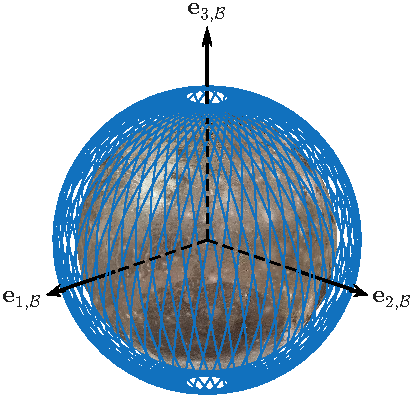
\includegraphics[width=.5\textwidth]{IMAGES/JUICE_orbit.pdf}

	%-----------
    \begin{overpic}[width=.5\textwidth]{IMAGES/JUICE_orbit.pdf}
        % e_1 axis label box
        \put(-1,23){%
            \colorbox{white}{$\vec{e}_{1,\mathcal{B}}$}%
        }
        % e_2 axis label box
        \put(89, 23){%
            \colorbox{white}{$\vec{e}_{2,\mathcal{B}}$}%
        }
        % e_3 axis label box
        \put(45, 92){%
            \colorbox{white}{$\vec{e}_{3,\mathcal{B}}$}%
        }
    \end{overpic}
	%------------
    \caption{Geometry of the Juice orbit during the GCO-500, as seen in the body-fixed frame of Ganymede over one orbital period.}
    \label{fig:Juice_orbit}
\end{figure}



%_____________________________________________________________
% 						FIGURE: EULER ANGLES & ORBITAL ELEMENTS
%_____________________________________________________________
\begin{figure}
	\centering


	\def\radius{3}
	\def\Alpha{180 + 32} %28
	\def\Alphashift{\Alpha-180}
	\def\Beta{25}
	\def\Gamma{100}

	\def\L{1}
	\def\Lnp{1}
	\def\radpngL{50}

	\tdplotsetmaincoords{70}{-7} %-2

	\tikzset{% Some styles
		axisint/.style={thin, -},
		axis/.style={thin, fill=black, -latex', shorten >=-10pt},
		dashaxis/.style={thin, fill=black, -latex', shorten >=-10pt, loosely dashed},
		behindline/.style={loosely dashed}
	}

	\begin{tikzpicture}[tdplot_main_coords, scale=\radius]


	\begin{scope}[every path/.style={tdplot_rotated_coords}]

	% Back half of the white circle.
	\tdplotsetrotatedcoords{\Alpha}{0}{0}
	\draw  [fill=white] 
		plot    [domain=90:270, samples=100] (cos \x, sin \x) -- cycle;

	% Dark gray circle
	\tdplotsetrotatedcoords{\Alpha+90}{90}{90}
	\draw [fill=gray!80, thin, domain=0:\Beta] 
		(0,0) -- plot (cos \x, sin \x) -- cycle;

	% The light gray circle
	\tdplotsetrotatedcoords{\Alpha}{\Beta}{\Gamma}
	\draw  [fill=gray!20] 
		plot    [domain=0:360, samples=100] (cos \x, sin \x);


	% The dashed edge of the back half of the white circle
	\begin{scope}
	\tdplotsetrotatedcoords{\Alpha}{\Beta}{\Gamma}
	\path  [clip] 
		plot    [domain=0:360, samples=100] (cos \x, sin \x);

	\tdplotsetrotatedcoords{\Alpha}{0}{0}
	\draw  [behindline] 
		plot    [domain=90:270, samples=100] (cos \x, sin \x);

	\end{scope}

	% The dark gray sector
	\tdplotsetrotatedcoords{\Alpha-90}{-90}{90}
	\draw [fill=gray!80, thin, domain=0:\Beta] 
		(0,0) -- plot (cos \x, sin \x) -- cycle;

	% Dashed light gray circle part 1
	\begin{scope}
	\tdplotsetrotatedcoords{\Alpha}{\Beta}{\Gamma}
	\draw  [behindline] 
		plot    [domain=0:360, samples=100] (cos \x, sin \x);
	\end{scope}

	% THETA (dark gray arc)
	\tdplotsetrotatedcoords{\Alpha+90}{90}{0}
	\tdplotdrawarc[->]{(0,0,0)}{.75}{-90}{-90+\Beta}{anchor=south, xshift=-6pt, yshift=-10pt}{}

	% The front half of the WHITE circle
	\tdplotsetrotatedcoords{\Alpha}{0}{0}  
	\draw  [fill=white] 
		plot [domain=-90:90, samples=100] (cos \x, sin \x) 
		-- cycle;


	% SMALL SPHERE (Ganymede)
		\shade[tdplot_screen_coords, ball color=brown!50] (0,0) circle (2pt);
		% Image overlay clipped in circle
		\begin{scope}[tdplot_screen_coords]
		%\clip (0,0) circle (10pt); % match circle size
		\node at (0,0) {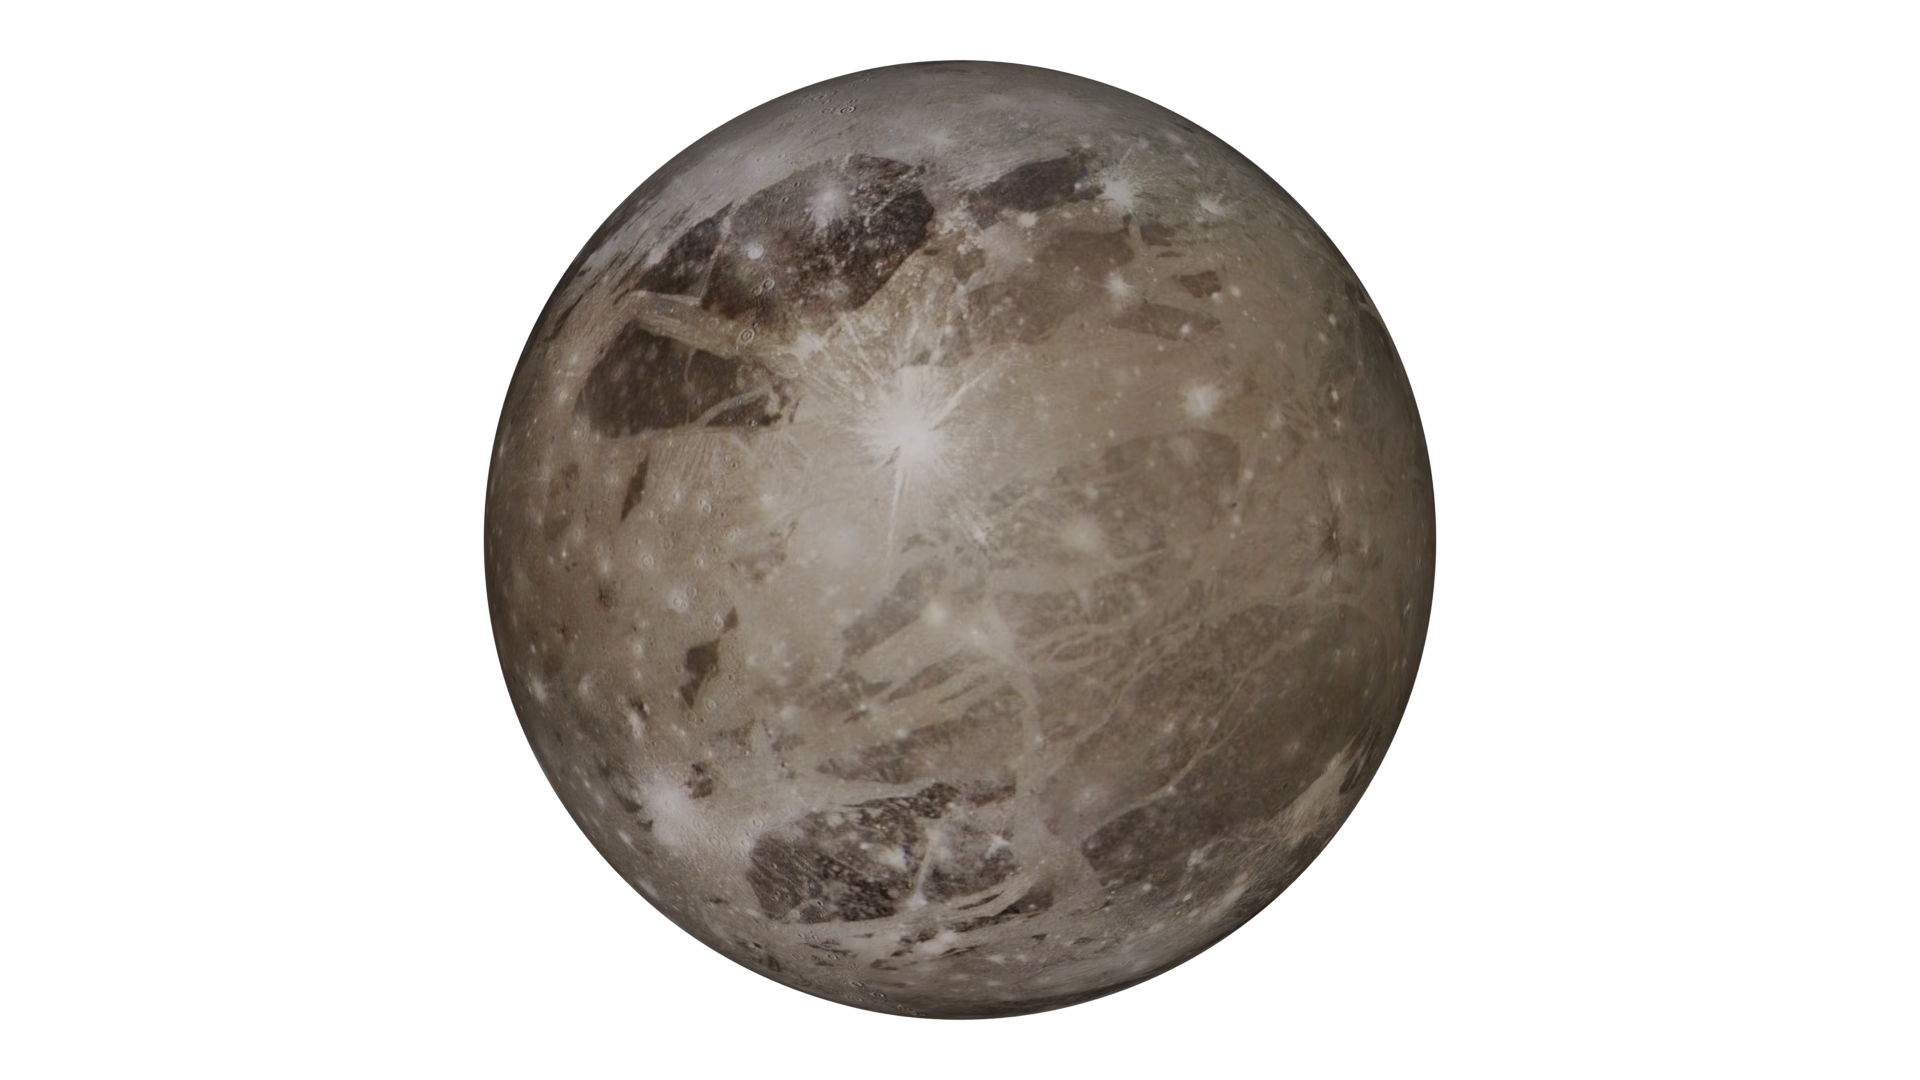
\includegraphics[width=\radpngL pt]{IMAGES/spheres/ganymede.png}};
		\end{scope}

	% The dashed lines in the front half of the white circle
	\begin{scope}
		\tdplotsetrotatedcoords{\Alpha}{0}{0}
		\path  [clip] 
			plot [domain=-90:90, samples=100] (cos \x, sin \x) 
			-- cycle;

		% Dashed light gray circle part 2
		\begin{scope}
		\tdplotsetrotatedcoords{\Alpha}{\Beta}{\Gamma}
		\draw  [behindline] 
			plot    [domain=0:360, samples=100] (cos \x, sin \x);
		\end{scope}

		\tdplotsetrotatedcoords{\Alpha-90}{-90}{90}
		\draw [behindline] (0,0) -- (cos \Beta, sin \Beta );

		\tdplotsetrotatedcoords{\Alpha}{\Beta}{\Gamma}
		\draw [behindline] (0,0,0) -- (1,0,0);

	\end{scope}

		
	% INERTIAL FRAME Axes
	\tdplotsetrotatedcoords{0}{0}{0}
	\draw[axis] (0,0,0) -- (0,-\L,0) node [anchor=north, xshift=0pt, yshift=-7pt]  {$\vec{e}_{1,\mathcal{I}}$};
	\draw[axis] (0,0,0) -- (\L,0,0) node [anchor=west, xshift=12pt, yshift=0pt] {$\vec{e}_{2,\mathcal{I}}$};
	\draw[axis] (0,0,0) -- (0,0,\L) node [anchor=north, xshift=0pt, yshift=+24pt] {$\vec{e}_{3,\mathcal{I}}$};

	% Laplace pole
	% \draw[axis] (0,0,0) -- (0,0,\Lnp) node [anchor=north, xshift=0pt, yshift=+22pt] {$\vec{p}$};

	% Orthogonal to the Line of NODES
	\tdplotsetrotatedcoords{\Alpha}{0}{0}
	\draw[axisint] (0,0,0) -- (1,0,0);
	\draw[behindline] (0,0,0) -- (-1,0,0); 

	% The BODY FIXED axes (care 1 and to are modified to compensate ZYZ to ZXZ order)
	\tdplotsetrotatedcoords{\Alpha}{\Beta}{\Gamma}
	\draw[axis] (0,0,0) -- (0,\L,0) node [anchor=north, xshift=10pt, yshift=20pt] {$\vec{e}_{1,\mathcal{B}}$};
	\draw[dashaxis] (0,0,0) -- (-\L,0,0) node [anchor=north, xshift=-22pt, yshift=13pt] {$\vec{e}_{2,\mathcal{B}}$};
	% \draw[axis] (0,0,0) -- (0,0,\L) node [anchor=east, xshift=-4pt, yshift=8pt] {$\vec{\omega}\vec{e}_{3,\mathcal{B}}$};
	\draw[axis] (0,0,0) -- (0,0,\L) node [anchor=north, xshift=-13pt, yshift=22pt] {$\vec{\omega} \approx \vec{e}_{3,\mathcal{B}} $};

	% Spin axis
	% \draw[axis] (0,0,0) -- (0,0,\Lnp) node [anchor=north, xshift=-6pt, yshift=20pt] {$\vec{\omega}$};

	
	% PHI
	\tdplotsetrotatedcoords{-90}{0}{0}
	\tdplotdrawarc[->]{(0,0,0)}{0.47}{0}{\Alphashift-1}{anchor=south, xshift=0pt, yshift=-13pt}{$\varphi$}
	% PSI
	\tdplotsetrotatedcoords{\Alpha}{\Beta}{\Gamma}
	\tdplotdrawarc[->]{(0,0,0)}{0.47}{90-\Gamma}{90}{anchor=south, xshift=7pt, yshift=-14pt}{$\psi$}
	% THETA (between BF axes)
	\tdplotsetrotatedcoords{\Alpha+90}{90}{0}
	\tdplotdrawarc[->]{(0,0,0)}{0.75}{-180}{-180+\Beta}{anchor=south, xshift=-1pt, yshift=0pt}{$\theta$}
	% THETA (dark sector)
	\tdplotsetrotatedcoords{\Alpha+90}{90}{0}
	\tdplotdrawarc[->, dashed]{(0,0,0)}{.75}{-90}{-90+\Beta}{anchor=south, xshift=-8pt, yshift=-12pt}{$\theta$}


	% % SNK vectors
	% \def\Lsnk{1.33*\L}

	% % S: spin
	% \tdplotsetrotatedcoords{\Alpha}{\Beta}{\Gamma}
	% \draw[axis] (0,0,0) -- (0,0,\Lsnk) node [anchor=east, xshift=-3pt, yshift=12pt] {$\vec{\omega}$};
	% % K: Laplace plane vector
	% \def\incl{10}
	% \tdplotsetrotatedcoords{\Alpha}{\Beta+\incl}{\Gamma}
	% \draw[axis] (0,0,0) -- (0,0,\Lsnk) node [anchor=east, xshift=-7pt, yshift=9pt] {$\vec{p}$};
	% % N: Orbit normal
	% \def\eps{5}
	% \tdplotsetrotatedcoords{\Alpha}{\Beta+\eps}{\Gamma}
	% \draw[axis] (0,0,0) -- (0,0,\Lsnk) node [anchor=east, xshift=-5pt, yshift=12pt] {$\vec{n}$};

	% % EPSILON: obliquity arc
	% \tdplotsetrotatedcoords{\Alpha+90}{90}{0}
	% \tdplotdrawarc[->]{(0,0,0)}{0.8}{-180+\Beta}{-180+\Beta + \eps}{anchor=south, xshift=-5pt, yshift=0pt}{$\epsilon$}

	% % I: incl arc
	% \tdplotsetrotatedcoords{\Alpha+90}{90}{0}
	% \tdplotdrawarc[->]{(0,0,0)}{0.88}{-180+\Beta+\eps}{-180+\Beta + \incl}{anchor=south, xshift=-5pt, yshift=-2pt}{$i$}

	% Arrows angles
	% PHI
	%\tdplotsetrotatedcoords{0}{0}{0}
	% \tdplotdrawarc[->, dashed]{(0,0,0)}{0.69}{0}{\Alphashift-1}{anchor=south, xshift=7pt, yshift=-4pt}{$\varphi$}

	% \tdplotsetrotatedcoords{\Alpha+90}{90}{0}
	% \tdplotdrawarc[->]{(0,0,0)}{.75}{-90}{-90+\Beta}{anchor=south, xshift=-6pt, yshift=-10pt}{$\theta$}

	% new theta
	% \tdplotsetrotatedcoords{\Alpha+90}{90}{0}
	% \tdplotdrawarc[->]{(0,0,0)}{0.8}{90}{90+\Beta}{left}{$\theta$}

	% \tdplotsetrotatedcoords{\Alpha}{\Beta}{\Gamma}
	% \tdplotdrawarc[->]{(0,0,0)}{0.8}{-\Gamma}{0}{below}{$\psi$}


	\end{scope}

	\end{tikzpicture}

	
	\caption{
	Schematic representation of the relations between the Euler angles, the inertial frame ${\mathcal{I}}$ centered on the satellite and the satellite's principal axis frame 
	${\mathcal{B}}$.
	}


\label{fig:tikz_orbital_euler_V2}
\end{figure}
%--------------------------------------------------------------------------------------


In this section we develop the set of differential equations that govern the rotational motion of the Galilean satellites, in the rigid-body approximation.
We consider a simplified model where the only torque acting on the satellites triaxial figure is due to the gravitational interaction with the point-mass Jupiter.
The influence of other moons, the Sun, and Jupiter's figure is accounted for indirectly through perturbations on the orbits of the Galilean satellites. The orbits of the Galilean satellites used in this work are taken from the latest JPL ephemerides for the Galilean satellites (JUP365). The differences with the most recent IMCCE ephemerides (NOE-5-2021) is of the order of few tens of kilometers \citep{2025Icar..42616344R}.


\subsection{Reference frames}\label{sec:reference_frames_V2}


In this section we describe the relations among the International Celestial Reference Frame (ICRF), and the body fixed frame attached to Ganymede.
%
The inertial frame adopted in this work is the third realization of the ICRF \citep{2020A&A...644A.159C},  that is adopted by the International Astronomical Union (IAU). 
Hereafter we will denote the ICRF and its axes as ${\mathcal{I} = 
\{\vec{e}_{1,\mathcal{I}},\vec{e}_{2,\mathcal{I}},\vec{e}_{3,\mathcal{I}}\}}$.
%
Now consider a right-handed body-fixed reference frame with origin coinciding with Ganymede's center of mass
\begin{equation}
{\mathcal{B} = 
\{\vec{e}_{1,\mathcal{B}},\vec{e}_{2,\mathcal{B}},\vec{e}_{3,\mathcal{B}}\}}.
\end{equation}
Such frame is defined based on some topographic features and such that $\vec{e}_{1,\mathcal{B}}$ points toward Jupiter, $\vec{e}_{3,\mathcal{B}}$ is the north pole, and $\vec{e}_{2,\mathcal{B}}$. Ideally such a frame coincides with the principal axes frame, in which case the axes are aligned with the bodies principal axes of inertia corresponding to the moments ${A_\mathrm{s} < B_\mathrm{s} < C_\mathrm{s}}$, respectively. 
In the following the moments of inertia $A_\mathrm{s}$, $B_\mathrm{s}$, $C_\mathrm{s}$ will always refer to those of its icy shell if a subsurface ocean is present or to the solid Ganymede if no ocean is present. Indeed if a subsurface ocean is present the rotation of the shell will be partially decoupled from that of the interior, and the observed rotational state will be that of the shell only.
%
If $\mathcal{B}$ is a principal reference frame for the rigid satellite, the products of inertia are zero and $\vec{I}$ becomes diagonal, that is,
%
\begin{equation}
	\vec{I} = 
	I_{ij} = 
	\begin{pmatrix}
		I_{11} & I_{12} & I_{13} \\
		I_{12} & I_{22} & I_{23} \\
		I_{13} & I_{23} & I_{33}
	\end{pmatrix}
	=
	\begin{pmatrix}
		A_\mathrm{s} & 0 & 0 \\
		0 & B_\mathrm{s} & 0 \\
		0 & 0 & C_\mathrm{s}
	\end{pmatrix}.
\end{equation}
%
Throughout this work we will refer interchangeably to the same moments as ${I_{11} < I_{22} < I_{33}}$ or ${A_\mathrm{s} < B_\mathrm{s} < C_\mathrm{s}}$, respectively.

The axis of minimum inertia ($A_\mathrm{s}$) is the one facing Jupiter and corresponds to the longest axis of the satellite's triaxial figure. Vice versa, the axis corresponding to the largest moment of inertia $(C_\mathrm{s})$ is the rotation axis and is pointing up relative the orbital plane. 
It is worth noting, the well known fact that stable rotation about the axis of intermediate inertia ($B$) is not possible \citep[see, e.g.,][]{Goldstein:102554}.
%
In practice, we cannot guarantee that the chosen frame coincides perfectly with the principal axes frame, and in general it will not. As more accurate measurements will lead to different realizations of the principal axes frame of the body. 
%
In the case of our Moon, the reference frame of choice for the production of maps and DTMs is the Mean Earth/Polar Axis system (ME frame), in use since before 1775 \citep[see, e.g.,][]{2000JGR...10520277D}, which is distinct from the Principal Axis system (PA frame). The PA frame is more suited for dynamical purposes and successive realizations will slightly differ as more data is acquired and changes in the gravity field occurs. The difference between the two frame is of several hundred meters, up to \SI{875}{m} on the surface. %(\SI{572}{m} in longitude).
In the following we will construct our framework by allowing for non-zero products of inertia, thus keeping the formulation as general as possible.
By including the off-diagonal terms of the inertia tensor in the estimation process we allow in principle to estimate the deviation between the topography defined body-fixed frame and the actual principal axes frame. Indeed, in principle, the rotation matrix between the two reference systems is the one that diagonalizes the inertia tensor in the chosen body-fixed frame.



%, which covers the years from 1600 to 2200, enough to capture one complete precession cycle of Callisto!
%
The Euler equations governing the angular velocities can be written as
\begin{equation}\label{eq:euler_solid_moon_williams_V2}
	\frac{d(\vec{I} \vec{\omega}_{\mathcal{B}})}{dt} + \vec{\omega}_{\mathcal{B}} \times(\vec{I} \vec{\omega}_{\mathcal{B}}) = \vec{k},
\end{equation}
%
where $\vec{I}$ is the moment is the satellite's inertia tensor, $\vec{\omega}_{\mathcal{B}}$ is the instantaneous spin or angular velocity vector,  $\vec{I} \vec{\omega}_{\mathcal{B}}$ is angular momentum vector, and $\vec{k}$ is the torque vector. 

%
In general, the satellite's inertia tensor varies over time due to tidal distortions from Jupiter, the Sun, other Galilean moons, and spin effects, we neglect these contributions to the rotational dynamics here.
%
The Euler equations are expressed in the body-fixed frame $\mathcal{B}$ using angular velocity components ${\vec{\omega}_{\mathcal{B}} = (\omega_1, \omega_2, \omega_3)^\top}$. 
The orientation of the satellite's body-fixed frame $\mathcal{B}$ relative to the inertial frame $\mathcal{I}$
is described in terms  of the 3-1-3 Euler angles, ${\vec{\varphi} = (\varphi, \theta, \psi)^\top}$.

Then the rotation that orients the principal axes frame $\mathcal{B}$ in the Laplace frame $\mathcal{I}$ to can be written as
\begin{equation}
	\vec{R}^{\mathcal{I}}_{\mathcal{B}} =
 	\vec{R}_{z}({\psi})
	\vec{R}_{x}(\theta)
	\vec{R}_{z}(\varphi)
	= \vec{R}({\varphi},{\theta},{\psi}),
\end{equation}
% %
% Similarly, we can define  ${({\varphi^\prime},{\theta^\prime},{\psi^\prime}})$,
% the 3-1-3 Euler angles that orient the principal axes relative to the $\mathcal{P}$ frame. 
% The relations between the two reference $\mathcal{I}$ and $\mathcal{P}$ frames, and the associated Euler angles is illustrated in Appendix~\ref{appendix:rotm_V2}.
% Then, the rotation that orients the principal axes frame $\mathcal{B}$ in the Laplace frame $\mathcal{P}$ to can be written as
% \begin{equation}
% 	\vec{R}^{\mathcal{P}}_{\mathcal{B}} =
% 	\vec{R}^{\mathcal{P}}_{\mathcal{I}} 
% 	\vec{R}_{\mathcal{B}}^{\mathcal{I}} = 
%  	\vec{R}_{z}({\psi^\prime})
% 	\vec{R}_{x}(\theta^\prime)
% 	\vec{R}_{z}(\varphi^\prime)
% 	= \vec{R}({\varphi^\prime},{\theta^\prime},{\psi^\prime}),
% \end{equation}
The precession angle ${\varphi}$ is the longitude of the ascending node of the satellite's equator in the inertial frame ($\mathcal{I}$), the nutation angle  ${\theta}$ is the inclination of the satellites' equator to the ICRF equator, and the rotation angle ${\psi}$ is the angle between the ascending node of the equator and body-fixed axis pointing toward Jupiter ($\vec{e}_{1,\mathcal{B}}$).
% The angles ${({\varphi^\prime},{\theta^\prime},{\psi^\prime}})$ can be interpreted geometrically as the precession, nutation, and rotation angles, in this order.
%
The reader is advised that often in the literature the symbols for first and third Euler angles are reversed \citep[e.g.,][]{1980A&A....82..129B, 1981M&P....25....3E}. Our notation is consistent with that of the IAU Working Group on Cartographic Coordinates and Rotational Elements \citep{2018CeMDA.130...22A}. %also with DE440 Park 2021
%
The relationship between the Euler angles and the reference frames $\mathcal{B}$ and $\mathcal{I}$ is illustrated in Fig.~\ref{fig:tikz_orbital_euler_V2}.
% Clearly, Fig.~\ref{fig:tikz_orbital_euler} illustrates also the relationship between the $\mathcal{B}$ and $\mathcal{I}$ frames if one replaces ${(\varphi^\prime, \theta^\prime, \psi^\prime)}$ with ${(\varphi, \theta, \psi)}$  and $\mathcal{P}$ with $\mathcal{I}$.


The 3-1-3 Euler angles rates $\dot{\vec{\varphi}}$ are related to the angular velocities, via the kinematic equations 
 %= (\dot{\varphi}, \dot{\theta}, \dot{\psi})^\top}$
 \begin{align} \label{eq:deuler_omega_V2}
	\vec{\omega}_{\mathcal{B}} = 
	% \begin{pmatrix}
	% 		\omega_1 \\
	% 		\omega_2 \\
	% 		\omega_3
	% 	\end{pmatrix} =
	\begin{pmatrix}
			\sin\theta \sin\psi  & \cos\psi & 0 \\
			\sin\theta \cos\psi &-\sin\psi & 0 \\
			\cos\theta & 0 &1 
	\end{pmatrix}
	\begin{pmatrix}
		\dot{\varphi} \\
		\dot{\theta} \\
		\dot{\psi}
	\end{pmatrix}
	= \vec{W}\dot{\vec{\varphi}},
\end{align}
%
The equation above clearly defines $\vec{W}(\theta,\psi)$.
Inverting Eq.~(\ref{eq:deuler_omega_V2}) we obtain the set of
first order ordinary differential equations (ODEs)
\begin{equation}\label{eq:deuler_omega_ODE_V2}
	\dot{\vec{\varphi}} = \vec{W}^{-1}\vec{\omega}_{\mathcal{B}}.
\end{equation} 


Notably, the equation above depends explicitly only on two of the three Euler angles.
However, Eqs.~(\ref{eq:euler_solid_moon_williams_V2}) and (\ref{eq:deuler_omega_ODE_V2}) are coupled through the torque $\vec{k}$ acting on the satellite, as this depends on its orientation in space relative to Jupiter.


The rate of change of the rotation angle $\dot{\psi}$ is much larger than the other two, so that the slowly varying spin axis $\vec{\omega}$ is nearly aligned with the axis of corresponding to the largest moment of inertia $\vec{e}_{3,\mathcal{B}}$ at all times. 


Since we are primarily interested in the satellite's orientation in an inertial frame  $\mathcal{I}$, we prefer to replace Eq.~(\ref{eq:euler_solid_moon_williams_V2}) with a set of second-order ODEs for the Euler angles alone. The derivation of the equations of motion presented here follows that \citet{Broucke1990doi:10.2514/3.20591}.
In virtue of Eq.~\eqref{eq:deuler_omega_V2}, the rotational kinetic energy can be written as
\begin{equation}\label{eq:rot_kinetic_energy_V2}
	\mathcal{T}  = 
	\tfrac{1}{2} \vec{\omega}_{\mathcal{B}}^\top \vec{I} \vec{\omega}_{\mathcal{B}} 
	= \tfrac{1}{2} \dot{\vec{\varphi}}^\top\vec{W}^\top \vec{I} \vec{W}\dot{\vec{\varphi}}.
\end{equation}
From Eq.~\eqref{eq:rot_kinetic_energy_V2} it is clear that the kinetic energy is a quadratic form in the Euler angle rates
${(\dot{\varphi},\dot{\theta},\dot{\psi})}$.

% The angular velocities with their expression in terms of the coordinates ${ \vec{\Phi} = ({\varphi}, {\theta}, {\psi} ) }$, and their time derivatives ${ \dot{\vec{\Phi}} }$, which can be readily obtained by inverting Eq.~(\ref{eq:deuler_omega_V2}).

Now let us identify ${q^1 = \varphi}$, ${q^2 = \theta}$, and ${q^3 = \psi}$. %so that $ \vec{\Phi} = (q^1, q^2, q^3)^\top$.
Denote by $\mathcal{U}$ the external mutual gravitational potential due to Jupiter and the satellite. 
Then, we can write the Lagrangian  in the form %${\mathcal{L} =\mathcal{T} + \mathcal{U}}$
%
\begin{equation}\label{eq:lagrangian_V2}
	\mathcal{L} =
	\mathcal{T} + \mathcal{U} =
	\tfrac{1}{2}	g_{\alpha\beta} \dot{q}^\alpha \dot{q}^\beta
	+ \mathcal{U},
	 %\frac{d{q^\alpha}}{dt}\frac{d{q^\beta}}{dt} %  \; k= 1, 2, 3$
\end{equation}
%
where we used Einstein summation convention. 
The metric tensor ${g_{\alpha\beta} = g_{\beta\alpha}}$ is symmetric, and its components  are functions of the Euler angles and of the components of the inertia tensor ${I}_{ij}$. The explicit expression of the metric tensor $g_{\alpha\beta}$ is given in Sect.~\ref{appendix:metric_tensor_off_diagonal}.

The equations for the Euler angles only that replace Eqs.~(\ref{eq:euler_solid_moon_williams_V2}) and (\ref{eq:deuler_omega_V2}) can be derived from the Lagrange equations
%
\begin{equation}
	\frac{d}{dt}\left(\frac{\partial \mathcal{L}}{\partial \dot{q}^\alpha}\right) - \frac{\partial \mathcal{L}}{\partial q^\alpha} = 0, \quad \alpha = 1, 2,3,
\end{equation}
%
where the Euler angles play the role of the generalized coordinates.
Proceeding as in  \citet{Broucke1990doi:10.2514/3.20591}, we can write
%
\begin{equation}\label{eq_geodesic_potential_V2}
	\ddot{q}^\alpha + 
	\Gamma^{\alpha}_{\beta\gamma} \dot{q}^\beta \dot{q}^\gamma =
	g^{\alpha\beta} \frac{\partial \mathcal{U}}{\partial q^\beta}, \quad \alpha = 1,2,3,
\end{equation}
%
where $g^{\alpha\beta}$ is the inverse metric tensor, that is, ${g^{\alpha\beta}  g_{\beta\gamma} = \delta_\alpha^\gamma}$, with $\delta_\alpha^\gamma$ being the identity tensor,
and we have introduced the Christoffel symbols of the second kind
%
\begin{equation} \label{eq:def_Christoffel_2nd_V2}
	\Gamma^\alpha_{\beta\gamma} = 
	g^{\alpha\lambda} \Gamma_{\beta\gamma\lambda}, %\quad 
	%\Gamma_{\beta\gamma\lambda} = 
	%  g^{\alpha\lambda}  \frac{1}{2} \left( \pdv{g_{\lambda\beta}}{q^\gamma} + \pdv{g_{\lambda\gamma}}{q^\beta} - \pdv{g_{\beta\gamma}}{q^\lambda} \right).
\end{equation}
where the Christoffel symbols of the first kind are defined as
\begin{equation} \label{eq:def_Christoffel_1st_V2}
	\Gamma_{\beta\gamma\lambda} = 
	 \frac{1}{2} \left( \pdv{g_{\lambda\beta}}{q^\gamma} + \pdv{g_{\lambda\gamma}}{q^\beta} - \pdv{g_{\beta\gamma}}{q^\lambda} \right).
\end{equation}
%
The explicit expression of the metric tensor components and the 27 Christoffel symbols of the first kind $\Gamma_{\alpha\beta\gamma}$ in terms of the Euler angles and moments of inertia ${I}_{ij}$ is given in Sect.~\ref{sec:metric_tensor_christoffel_off_diagonal}.
Equation~(\ref{eq_geodesic_potential_V2}) is the desired set of second order ODEs for the Euler angles.
Since only the derivatives with respect to the Euler angles appear on the right-hand side of Eq.~(\ref{eq_geodesic_potential_V2}), it is clear that the only contribution of the potential $\mathcal{U}$, on the orientation must come from Euler angles dependent terms.
%
It remains to provide an explicit expression for the potential $\mathcal{U}$.
Assume for the moment that all internal layers are solid, aligned, and strongly coupled gravitationally, allowing the Galilean satellites to be treated as rigid bodies. Consequently, we neglect internal coupling mechanisms and consider only the effects of the external gravitational potential.
% %
% However, it must be emphasized that this assumption is likely not representative of the actual interior structure. A subsurface liquid ocean is thought to exist beneath the icy shells of Ganymede and Europa, and possibly also Callisto. Conversely, Io may host a magma ocean, sustained by intense tidal heating due to its proximity to Jupiter, although recent studies suggest that it does not \citep{2025Natur.638...69P}.
% %
% Previous modelling efforts have accounted for the influence of a subsurface ocean on longitudinal librations \citep[e.g.,][]{2010Icar..209..651B, 2011A&A...527A.118R} and obliquity \citep[e.g.,][]{2012Icar..220..435B}. 
% Our present aim is to compare the response of linearized rigid-body models for librations and obliquity of the Galilean satellites with predictions from our triaxial model.
%
% Future work should extend the present framework to incorporate the effects of internal liquid layers in the rotational dynamics and Euler angle equations.

In general the expression for the mutual potential between two extended bodies is rather cumbersome, \citep[see, e.g.,][]{1978CeMec..18..295B, Tricarico2008CeMDA.100..319T}. Here for simplicity  only the McCullagh potential due to the interaction of  a point mass with the degree-two field of Ganymede. 
However, the interaction between $J_2$ of Jupiter with the degree-two field of the satellite may be important \citep[see, e.g.,][]{1981M&P....25....3E}. 
The McCullagh potential expressed in terms of the satellite's gravity coefficients of degree-two can be written 
%
\begin{equation}\label{potential_1b_approx_stokes_V2}
	\mathcal{U} = 	\mathcal{G}
	\left(
	\frac{M_{\mathrm{J}} {M}_{\mathrm{G}}}{r} 
	+ M_{\mathrm{J}} {M}_{\mathrm{G}} R_\mathrm{G}^2 \frac{
		 \vec{r}^\top \left( 
	\vec{R}^\top \vec{Q} \vec{R}
		\right) \vec{r}}{2 r^5}
	 \right),
\end{equation}
%
where $\mathcal{G}$ is the gravitational constant,  $M_{\mathrm{J}}$ and ${M}_{\mathrm{G}}$ are the masses of Jupiter and Ganymede, respectively, $R_{\mathrm{G}}$ is Ganymedes's reference radius, 
$\vec{r}$ and $r$ are the relative position vector of the satellite with respect to Jupiter expressed in the $\mathcal{I}$ frame, and its magnitude, respectively.   
${\vec{R}(\varphi,\theta,\psi) = \vec{R}_{\mathcal{B}}^{\mathcal{I}}}$
is the rotation matrix from the inertial frame $\mathcal{I}$ to the body-fixed $\mathcal{B}$ frame, as defined in Appendix~\ref{appendix:rotm_V2}. 
We have also introduced the traceless quadrupole moment tensor \citep[e.g.,][]{Marchenko2001}
%
\begin{equation}
	\label{eq:def_Q_gravity_coeffs_V2}
	\vec{Q}  = 
	\begin{pmatrix}
		6C_{22} -C_{20} & 6 S_{22}& 3C_{21} \\
	6 S_{22}	& -6C_{22} - C_{20} & 3S_{21}  \\
	3C_{21}	&3S_{21}  & 2C_{20}
	\end{pmatrix}, 
\end{equation}
%
where the second degree Stokes coefficients $C_{2m}, S_{2m}$, in the rigid body approximation, are related to the moments of inertia by
%
\begin{subequations}
	\label{eq:inertia2stokes_V2}
\begin{align}
	\label{eq:inertia2stokes_V2_C20_V2}
	C_{20}  &= \frac{I_{11} + I_{22} - 2 I_{33} }{2{m}_\mathrm{G}R_\mathrm{G}^2}, \\ %\quad
	\label{eq:inertia2stokes_V2_C22_V2}
	C_{22}  &= \frac{I_{22} - I_{11}  }{4{m}_\mathrm{G}R_\mathrm{G}^2}, \\
	\label{eq:inertia2stokes_V2_C21_S21_S22_V2}
	C_{21}  &=-  \frac{ I_{13} }{{M}_{\mathrm{G}}R_\mathrm{G}^2}, \\%\quad
	S_{21}  &=-  \frac{ I_{32} }{{M}_{\mathrm{G}}R_\mathrm{G}^2}, \\% \quad
	S_{22}  &=-  \frac{ I_{21} }{2{m}_\mathrm{G}R_\mathrm{G}^2}. 
\end{align}
\end{subequations}
%
It is easy to verify that $\vec{Q}$ is related to the whole body inertia tensor, or that of the shell if the interior is assumed spherically symmetric, by
\begin{equation}\label{eq:Q2I_V2}
	\vec{Q} =
	 \frac{1}{{M}_{\mathrm{G}}R_\mathrm{G}^2}\left( \tr(\vec{I})\vec{1}_{3\times 3} - 3 \vec{I} \right)
\end{equation} 
%
If $\mathcal{B}$ is a principal axes frame and spin and tidal distortion are neglected, it holds ${C_{21} = S_{21} = S_{22} = 0}$.
% In general it is
% \begin{equation}
% 	\vec{I} = \tfrac{1}{3} \mathrm{tr}(\vec{I}) - \tfrac{1}{3}  {M}_{\mathrm{G}}R_\mathrm{G}^2 \vec{Q}.
% \end{equation}
%
Substituting this expression for the potential of Eq.~\eqref{potential_1b_approx_stokes_V2} in Eq.~(\ref{eq_geodesic_potential_V2}) we obtain 
%
\begin{equation}\label{eq:geodesic_explicit_V2}
	\ddot{q}^\alpha + 
	\Gamma^{\alpha}_{\beta\gamma} \dot{q}^\beta \dot{q}^\gamma =
	g^{\alpha\beta}
	\left(  
	\frac{\mathcal{G} \, M_{\mathrm{J}} {M}_{\mathrm{G}}R_\mathrm{G}^2 }{2 r^5}  \,
	\vec{r}^\top  \frac{\partial (\vec{R}^\top \vec{Q} \vec{R})}{\partial q^\beta} 
	{\vec{r}} 
	\right), %\;  \alpha = 1,2,3,
	% \left(   \displaystyle\sum_i
	% \frac{3G \, M_i}{2 r_i^5}  \,
	% \vec{r}_i^\top  \frac{\partial (\vec{R}\vec{I} \vec{R}^\top)}{\partial q^\beta} 
	% {\vec{r}_i} 
	% \right), \;  \alpha = 1,2,3.
\end{equation}
%
%where the partial derivatives of $\mathcal{U}$ with respect to the Euler angles are computed using the expression in Eq.~(\ref{eq:Christoffel_1st_kind}). 
where the partial derivatives with respect to the Euler angles $q^\alpha$ can be readily computed from the explicit expression of the rotation matrix $\vec{R}$, given in Appendix~\ref{appendix:rotm_V2}.
%


It is well known that the rotational equations for the rigid body and a torque arising from a McCullagh-like potential, actually depend only on the ratios of the moments of inertia.
Indeed, Eq.~\eqref{eq:geodesic_explicit_V2} is invariant under an arbitrary rescaling of the inertia tensor, that is ${\vec{I} \rightarrow c \vec{I}}$, with $c$ being some positive real number. 
Thus, the rotational equations are often rewritten in terms of the relative moments of inertia differences,
%
\begin{subequations}
\begin{align}
\alpha &= \frac{C_\mathrm{s} - B_\mathrm{s}}{A_\mathrm{s}}, \\%\quad
\beta &= \frac{C_\mathrm{s} - A_\mathrm{s}}{B_\mathrm{s}}, \\ %\quad
\gamma &= \frac{B_\mathrm{s} - A_\mathrm{s}}{C_\mathrm{s}} 
= \frac{\alpha\beta}{1-\alpha\beta}.
\end{align}
\end{subequations}
%
Since ${A_\mathrm{s}<B_\mathrm{s}<C_\mathrm{s}}$, these ratios are all positive quantities.
Clearly, only two of these three parameters are independent, and are required to integrate the rotational equations \citep{1965AJ.....70..466E}.
%
% ----------------- ADDED ----------------------------------
In this work however, the quadrupole coefficients in the McCullagh potential $\mathcal{U}$ are treated as independent constants rather than functions of the moments of inertia, which breaks the scale degeneracy. This allows for the independent estimation of the moments of inertia by directly injecting the gravity coefficients into the equations. While this means the relations in Eq.~\ref{eq:inertia2stokes_V2} are not explicitly enforced, it is not an inconsistency. In this framework, the moments of inertia represent only the outer shell, not the whole body; therefore, Eq.~\ref{eq:inertia2stokes_V2} would only hold if the interior were spherically symmetric.
%
Since we cannot guarantee a priori that the body-fixed reference frame to which the stereo DTM is attached is the principal axis frame, and almost certainly it is not, as it is usually chosen to be attached to some feature on the surface of the satellite. 
For this reason, it can be expected that the products of inertia (i.e., $I_{12}$,  $I_{13}$, and  $I_{23}$) are small but non-zero in the body-fixed frame. We choose to not estimate these parameters but to include them as consider parameters. This is explained in more detail in Sect.~\ref{sec:consider_covariance}.

% Since the tensor of inertia is not diagonal the metric tensor and the Christoffel symbols contain additional terms with respect to those obtained in Sect.~\ref{appendix:metric_tensor} where we assumed a principal frame (and no tidal deformations of the inertia tensor). The complete expression of the metric tensor and Christoffel symbol is given in Sect.~\ref{sec:metric_tensor_christoffel_off_diagonal}.
% --------------------------------------------------------------------


%
% In this work however, we choose to keep fixed the moment of inertia differences in the form of the gravity field coefficients of second degree of Eq.~\eqref{eq:inertia2stokes_V2_C20_C22}. 
% %
% In Table~\ref{tab:galilean_satellites_parameters_ext} we show the estimates of the values of $C_{20}$ and $C_{22}$ for each of the Galilean satellites, as well as the estimate for the value of the normalized polar moment of inertia, that is, ${C/({M}_{\mathrm{G}}R_{\mathrm{G}}^2)}$, obtained assuming hydrostatic equilibrium.
% These values are used together with Eq.~\eqref{eq:inertia2stokes_V2_C20_C22} to compute the values of the moments of inertia $A$, $B$, and $C$ used in the numerical integration of Eq.~\eqref{eq:geodesic_explicit}.
% %
% We denoted by $n$ the mean motion of the satellite, while ${T_{n} = 2\pi / n }$ represents its  mean orbital period.
% Throughout the text we will use subscript indices $\mathrm{G}$ from 1 through 4, are used to refer to the Galilean satellites: Io, Europa, Ganymede, and Callisto, in this order. For simplicity, subscripts will often be omitted when doing so does not create any ambiguity.

The differential equations are numerically integrated using an adaptive Runge-Kutta method of order 9, with an embedded 8th-order error estimate \citep{Verner2010}. % Runge-Kutta $9(8)$ pair




%----------------------------------------------------------------------------
%------------ CHAPTER OCEAN COUPLING ----------------------------------------
%----------------------------------------------------------------------------
\subsection{Shell-ocean coupling}\label{sec:ocean_rayleigh_V2}

% \section{Rotational equations with ocean coupling}\ref{sec_rotational_eqs_ocean}
% Read also: \cite{2023JGRE..12807648H}.

In this section, we extend the rotational model to include the effects of coupling between a solid outer layer and a subsurface fluid layer. This configuration is applicable to the outer shell of an icy satellite overlying a subsurface ocean, or the lunar mantle interacting with a liquid core.
For simplicity, we assume the boundary between the solid and liquid layers to be spherical.
%
We denote the angular velocity of the outer solid layer in the body fixed frame as ${\vec{\omega} = \vec{\omega}_\mathcal{B}}$, and that of the liquid layer by $\vec{\omega}_{\mathrm{o}}$. We also introduce the angular velocity difference ${\Delta \vec{\omega} = \vec{\omega}_{\mathrm{o}} -  \vec{\omega}}$.


% \subsection{Viscous laminar boundary layer}
The interaction between the fluid layer and the solid shell is modeled by introducing an additional torque, $\vec{k}_{\mathrm{o}}$, to the right-hand side of Eq.~\eqref{eq:euler_solid_moon_williams_V2}. 
%
We consider a laminar coupling the solid-liquid boundary, in which case the torque can be written as \citep{1981RSPTA.303..327Y} %see eq 40 of Williams 2011.
%
\begin{equation}
	\vec{k}_{\mathrm{o}} =
	k_\mathrm{o}  \Delta \vec{\omega},
\end{equation}
%
where the constant coupling term has the form \citep{1981RSPTA.303..327Y, 1995Icar..117..250Y, 1968JFM....33..739B, 1965PCPS...61..279R}
\begin{equation}
	\label{eq:ocean_damping_coeff_laminar_V2}
	k_\mathrm{o} = 2.620  \frac{C_\mathrm{o} \sqrt{\nu_\mathrm{o} n}}{R_\mathrm{o}}
\end{equation}
where $R_\mathrm{o}$ is the radius of the liquid layer, $\nu_\mathrm{o}$ is the fluid kinematic viscosity, $C_\mathrm{o}$ is the polar moment of inertia of the ocean, and we approximated the angular velocity of the ocean layer can be approximated as $\|\vec{\omega}_\mathrm{o}\| \approx n$.
The dimensions of $k_\mathrm{o}$ are that of the moment of inertia per unit time, that is $\unit{kg.m^2.s^-1}$ in the International System of Units (SI).
%
We adopt a nominal kinematic viscosity of $\nu_\mathrm{o} = \SI{1.67e-6}{m^2.s^{-1}}$ as an initial baseline, which corresponds approximately to cold, liquid water at atmospheric pressure. Beneath the thick ice shell of an icy moon, the ocean exists at high hydrostatic pressures and likely contains dissolved salts, both of which will alter the true viscosity profile. Because the exact thermodynamic state and composition of the subsurface ocean are unknown, the actual value of $\nu_\mathrm{o}$ is highly uncertain. Consequently, rather than assuming this nominal value is exact, the bulk parameter $k_\mathrm{o}$ is treated as a considered parameter, and its formal uncertainty, set at $\num{e-10}C_\mathrm{s}\,\unit{s^{-1}}$, is propagated into the estimates of the other system parameters as described in Sect.~\ref{sec:consider_covariance}.

This formulation assumes a smooth boundary, as topographic irregularities on the core-mantle
boundary can give rise to additional stresses, which may play a dominant role \citep[see e.g.,][]{1981RSPTA.303..327Y}.
%
In the Lagrangian formalism, this torque is accounted for via a Rayleigh dissipation function, of the form
\begin{align}
\mathcal{F} &= \frac{k_\mathrm{o}}{2}  \| \Delta \vec{\omega} \|^2
= 
\frac{k_\mathrm{o}}{2}  \| \vec{W}_{\mathrm{o}}\dot{\vec{\varphi}}_{\mathrm{o}} - \vec{W}\dot{\vec{\varphi}} \|^2,
\end{align}
%
where the $\dot{\vec{\varphi}}_{\mathrm{o}}$ is the vector of Euler angles that define the orientation of the liquid layer, and the corresponding $\vec{W}_{\mathrm{o}}$ is defined in analogy to Eq.~\eqref{eq:deuler_omega_V2}.
%
The equations for the Euler angles can be derived from the Lagrange equations with Rayleigh dissipation, which read
%
\begin{equation}
	\frac{d}{dt}\left(\frac{\partial \mathcal{L}}{\partial \dot{q}^\alpha}\right) - \frac{\partial \mathcal{L}}{\partial q^\alpha}  
+ \frac{\partial \mathcal{F}}{\partial \dot{q}^\alpha}= 0, \quad \alpha = 1, 2,3,
\end{equation}
%
%
%
Finally, the equations of motion can be written as
\begin{equation}\label{eq:geodesic_potential_ocean_V2}
	\ddot{q}^\alpha + 
	\Gamma^{\alpha}_{\beta\gamma} \dot{q}^\beta \dot{q}^\gamma =
	g^{\alpha\beta} \left( \frac{\partial \mathcal{U}}{\partial q^\beta} - \frac{\partial \mathcal{F}}{\partial \dot{q}^\beta} \right), \quad \alpha = 1,2,3,
\end{equation}


In principle, one could numerically integrate the rotational equations for the ocean layer's Euler angles alongside those that govern the shell orientation, and the two sets of equations would be coupled. However, this requires specifying initial conditions for the ocean's orientation and rates, which constitutes a non-trivial task. 
We can assume that the spin axis of the ocean will exhibit some form of precession analogous to that of the shell, however,
\cite{1967JGR....72.3135G} concluded for the Moon that the coupling between the lunar mantle and its liquid core is too weak to align the solid and fluid rotational axes. % from Williams 2001
%
For simplicity, we will assume that the ocean layer rotates uniformly with zero obliquity, such that its angular velocity vector aligned with the orbit normal, with a constant magnitude equal to the mean motion $n$.

%%NB: Weak coupling remain closer to the ecliptic normal than the precessing the core spin axis is more nearly coincident with the precessing mantle (Yoder 1981)
%%NB: There are three excitation mechanisms that could plausibly excite the free librations lunar figure; moonquakes, impacts and turbulent core-mantle friction (Yoder 1981)



% %----------------- TURBULENT BOUNDARY LAYER FORMULATION -----------------
% \subsection{Turbulent boundary layer}

% \cite{1981RSPTA.303..327Y} showed that a coupling constant corresponding to a viscous laminar flow is inadequate to explain the Moon's observations. 
% Following \cite{2001JGR...10627933W}, we consider a
% turbulent stress at the boundary, in which case the torque can be defined as: %see eq 40 of Williams 2011.
% %
% \begin{equation}
% 	\vec{k}_{\mathrm{o}} = 
% 	k_\mathrm{o, turb} 
% 	\| \Delta \vec{\omega}\| \Delta \vec{\omega},
% \end{equation}
% %
% where the constant coupling term has the form
% \begin{equation}
% 	k_\mathrm{o, turb} = \frac{3}{4} \pi^2 \kappa \bar{\rho}_\mathrm{o} R_\mathrm{o}^5,
% \end{equation}
% where $R_\mathrm{o}$ is the radius of the liquid layer, $\bar{\rho}_\mathrm{o}$ is the fluid density,  and $\kappa$ is a dimensionless parameter which depends on the viscosity of the fluid. 
% The dimensions of $k_\mathrm{o, turb}$ are those of the moments of inertia, that is $\unit{kg.m^2}$, in SI units.
% %
% The corresponding Rayleigh dissipation function can be written as
% \begin{align}
% \mathcal{F} &= \frac{k_\mathrm{o, turb}}{3}  \| \Delta \vec{\omega} \|^3
% = 
% \frac{k_\mathrm{o, turb}}{3}  \| \vec{W}_{\mathrm{o}}\dot{\vec{\varphi}}_{\mathrm{o}} - \vec{W}\dot{\vec{\varphi}} \|^3.
% \end{align}


%--------------------------------------------------------------------------------

% \section{Rotational equations}\label{sec:rotational_eqs_extended}

% The reference frames used in this chapter are the same as that presented in Sect.~\ref{sec:reference_frames}.
% %
% The rotational equations are consistent with those presented in Sect.~\ref{sec:rotational_eqs} and extended in Chapter~\ref{sec:ocean_rayleigh}; however, we generalize them by allowing for a non-diagonal inertia tensor. Consequently, the body-fixed frame need not coincide with the principal axis frame. Furthermore, the quadrupole coefficients in the McCullagh potential $\mathcal{U}$ are treated as independent constants rather than functions of the moments of inertia. This allows for the independent estimation of the moments of inertia by directly injecting the gravity coefficients into the equations. While this means the relations in Eq.~\ref{eq:inertia2stokes_V2_C20_C22} are not explicitly enforced, it is not an inconsistency. In this framework, the moments of inertia represent only the outer shell, not the whole body; therefore, Eq.~\ref{eq:inertia2stokes_V2_C20_C22} would only hold if the interior were spherically symmetric.
% %
% The reason we include the products on inertia to the set of parameters to estimate is that we cannot guarantee a priori that the body-fixed reference frame to which the stereo DTM is attached is the principal axis frame, and almost certainly it is not, as it is usually chosen to be attached to some feature on the surface. 
% Since the tensor of inertia is not diagonal the metric tensor and the Christoffel symbols contain additional terms with respect to those obtained in Sect.~\ref{appendix:metric_tensor} where we assumed a principal frame (and no tidal deformations of the inertia tensor). The complete expression of the metric tensor and Christoffel symbol is given in Sect.~\ref{sec:metric_tensor_christoffel_off_diagonal}.





%---------------------------------------------------------------------------
\section{Estimation framework}\label{sec:DC_laser}
Consider the state vector of the rotating rigid body in the inertial frame
\begin{equation}
	\vec{x} = 
		( \vec{\varphi}, \dot{\vec{\varphi}})^\top = %\vec{x}, \dot{\vec{x}}
		(\varphi,\theta,\psi,\dot{\varphi},\dot{\theta},\dot{\psi}
		% ,x,y,z,\dot{x},\dot{y},\dot{z}
		)^\top, 
\end{equation}
and let  $\vec{p} = (I_{11}, I_{22}, I_{33}, I_{12}, I_{13}, I_{23}, k_\mathrm{o}) $,
%, \lambda_2,  0.0 \lambda_5]^\top$
be the  vector of constant parameters describing the force model $ \vec{F}(\vec{x}, \vec{p}, t ) $, in this case the moments and products of inertia of Ganymede's ice shell.
%, or the mantle in case of the Moon or Mercury. 
%
For compactness, we will write as usual $(\varphi,\theta,\psi)=(q^1,q^2,q^3)$.
%, and $(x,y,z) = (x_1,x_2,x_3)$.
%
\begin{equation}\label{eom}
	\dot{\vec{x} } = \frac{d}{dt}
	\begin{pmatrix}
		\vec{\varphi} \\
		\dot{\vec{\varphi}}
		%\\
		% \vec{x}\\
		% \dot{\vec{x}}
	\end{pmatrix}
	= \vec{F}(\vec{x}, \vec{p}, t ),
	\quad \vec{x}(t_0) = \vec{x}_0,
\end{equation}
where 
\begin{align}
	\vec{F} &= 
	\begin{pmatrix}
	\dot{q}^1 \\ \dot{q}^2 \\ \dot{q}^3 \\
	-{\Gamma}^{1}_{\beta\gamma} \dot{q}^\beta \dot{q}^\gamma 
	+{g}^{1\beta} 
	\left(
	\frac{\partial \mathcal{U}}{\partial q^\beta}
	 - \frac{\partial \mathcal{F}}{\partial \dot{q}^\beta} 
	\right)
	\\%
	-{\Gamma}^{2}_{\beta\gamma} \dot{q}^\beta \dot{q}^\gamma 
	+{g}^{2\beta} 
	\left(
	\frac{\partial \mathcal{U}}{\partial q^\beta} 
	- \frac{\partial \mathcal{F}}{\partial \dot{q}^\beta} 
	\right)
	\\ 
	-{\Gamma}^{3}_{\beta\gamma} \dot{q}^\beta \dot{q}^\gamma 
	+{g}^{3\beta} 
	\left(
	\frac{\partial \mathcal{U}}{\partial q^\beta}
	- \frac{\partial \mathcal{F}}{\partial \dot{q}^\beta} 
	\right)
	\end{pmatrix}.
\end{align}
% 
In general the observations  can be modeled by a function ${G}_{\mathrm{LA}}(\vec{x}, \vec{g}, t )$, depending on the state vector and the vector $\vec{g}$ of constant, non-dynamical, geometrical parameters, that is
%
\begin{equation}\label{Y_eq1}
	{y}(t) = {G}_{\mathrm{LA}}(\vec{x}, \vec{g}, t ) + \varepsilon(t), %cov??
\end{equation}
%
where 
% ${y}(t)$ is the $p$-dimensional vector of the range observations,
$\varepsilon(t)$ is the vector of measurement errors.
In the following geometrical parameters will include only $h_2$ Love number, that is $\vec{g} = h_2$. Nonetheless, we feel it is best to keep the notation slightly more general.
%Note that we require $p<n$ at any time epoch, that is fewer observations than there are state vector components. 
	

If a reasonable reference trajectory is available and if $\vec{x}$, the true trajectory, and $\vec{x}^*$,
the reference trajectory, remain sufficiently close throughout the time interval of interest, then the trajectory for the actual motion can be expanded in a Taylor's series about the reference trajectory at each point in time. If this expansion is truncated to eliminate higher order terms, then the deviation in the state from the reference trajectory can be described by a set of linear differential equations with time dependent coefficients. A linear relation between the observation deviation and the state deviation can be obtained by a similar expansion procedure. Then, the nonlinear problem in which the complete state vector is to be estimated can be replaced by a linear orbit determination problem in which the deviation from some reference solution is to be determined.
We assume that a reference solution $\vec{x}^* (t, \vec{x}_0 , \vec{p}^* )$ of the dynamical equations is known in terms of a set of reference values $\vec{p}^*$. The measurement model is likewise assumed to be known in terms of a set of reference values of the parameters $\vec{g}^*$. 
The goal here is to use a discrete set of measurements ${{y}(t_i) = {y}_i}$, to obtain improved values for the initial state $\vec{x}_0$ and the dynamical $\vec{p}^*$ and geometrical $\vec{g}^*$ parameters.
%
If we introduce the variations \( \delta \vec{x} \), \( \delta {y} \), \( \delta \vec{p} \), \( \delta \vec{g} \) of the state vector, the observations, and the parameters so that
%
\begin{subequations}
\begin{align}
	\vec{x}(t) &= \vec{x}^*(t, \vec{p}^*) + \delta \vec{x}, \\
	{y}_i(t) &= {G}_{\mathrm{LA}}(\vec{x}^*, \vec{g}^*, t_i) + \delta {y}_i, \\
	\vec{p} &= \vec{p}^* + \delta \vec{p}, \\
	\vec{g} &= \vec{g}^* + \delta \vec{g}.
\end{align}
\end{subequations}
%
A first-order expansion of the force ${ \vec{F}(\vec{x}, \vec{p}, t ) }$ and measurement model ${ {G}_{\mathrm{LA}}(\vec{x}, \vec{g}, t ) }$ yields
% \begin{subequations}
% 	\begin{align}
% 		\vec{F}(\vec{x}, \vec{p}, t ) &=  \vec{F}(\vec{x}^*, \vec{p}^*, t )
% 		+ \pdv{ \vec{F}}{ \vec{x}} \bigg|^* \delta \vec{x}(t) 
% 		+\pdv{ \vec{F}}{ \vec{p}} \bigg|^* \delta \vec{p}(t), \\
% 		{G}_{\mathrm{LA}}(\vec{x}, \vec{g}, t_i ) &=  {G}_{\mathrm{LA}}(\vec{x}^*, \vec{g}^*, t_i )
% 		+ \pdv{ {G}_{\mathrm{LA}}}{ \vec{x}} \bigg|^* \delta \vec{x}(t_i),
% 		+\pdv{ {G}_{\mathrm{LA}}}{ \vec{g}} \bigg|^* \delta \vec{g}(t_i).
% 	\end{align}
% \end{subequations}
%
\begin{subequations}
\begin{align}
\vec{F}(\vec{x}, \vec{p}, t)
&= \vec{F}(\vec{x}^*, \vec{p}^*, t)
+ \pdv{\vec{F}}{\vec{x}} \bigg|^* \delta \vec{x}(t) \notag\\
&\quad + \pdv{\vec{F}}{\vec{p}} \bigg|^* \delta \vec{p}(t), \\
{G}_{\mathrm{LA}}(\vec{x}, \vec{g}, t_i)
&= {G}_{\mathrm{LA}}(\vec{x}^*, \vec{g}^*, t_i)
+ \pdv{{G}_{\mathrm{LA}}}{\vec{x}} \bigg|^* \delta \vec{x}(t_i) \notag\\
&\quad + \pdv{{G}_{\mathrm{LA}}}{\vec{g}} \bigg|^* \delta \vec{g}(t_i).
\end{align}
\end{subequations}
%
Substitution into Eqs.~\eqref{eom} and \eqref{Y_eq1} yields the equations of the differential dynamics, or the state deviation vector and the differential measurement, in the form
\begin{align}\label{ve_1}
	\delta\dot{\vec{x}}(t) &= \pdv{\vec{F}}{\vec{x}}\bigg|^* \delta \vec{x}(t) + \pdv{\vec{F}}{\vec{p}}\bigg|^* \delta \vec{p}, \\
	\label{ve_2}
	\delta {y}_i &= \pdv{{G}_{\mathrm{LA}}}{\vec{x}} \bigg|^*\delta \vec{x}(t_i) + \pdv{{G}_{\mathrm{LA}}}{\vec{g}}\bigg|^* \delta \vec{g} 
	+ \varepsilon_i.
\end{align}
%
We define
\begin{subequations}
	\begin{align}
	\vec{A}(t) = \pdv{\vec{F}}{\vec{x}}\bigg|^*, \quad 
	\vec{B}(t) = \pdv{\vec{F}}{\vec{p}}\bigg|^*, \\ %\quad 
	\tilde{\vec{H}}_i = \pdv{{G}_{\mathrm{LA}}}{\vec{x}}\bigg|^*_i.
	\quad 
	\vec{H}^{\vec{g}}_i = \pdv{{G}_{\mathrm{LA}}}{\vec{g}}\bigg|^*_i.
	\end{align}
\end{subequations}
%
Then, Eqs.~\eqref{ve_1} and  \eqref{ve_2} can be rewritten as
%
\begin{subequations}
	\begin{align}\label{vareq_ext_v2}
		\delta \dot{\vec{x}}(t) &= \vec{A}(t) \delta \vec{x}(t) + \vec{B}(t) \delta \vec{p},
		\\
		\delta {y}_i &= \tilde{\vec{H}}_i \delta \vec{x}_i 
		+ \vec{H}^{\vec{g}}_i \delta \vec{g}
		+ \varepsilon_i,
		%\quad i = 1, \dots, l
	\end{align}
\end{subequations}
%
Note that Eq.~\eqref{vareq_ext_v2} is the variational equation associated with Eq.~\eqref{eom} extended to include the system parameters. %${\vec{p} = (I_{11}, I_{22}, I_{33}, I_{12}, I_{13}, I_{23}, k_\mathrm{o})}$.
We now write the explicit expression of the matrices of partial derivatives defined above.


\setcounter{MaxMatrixCols}{12}
\begin{align}
\vec{A}(t)=
% \begin{bmatrix}
% \frac{\partial f_1}{\partial \varphi} & \frac{\partial f_1}{\partial \theta} & \frac{\partial f_1}{\partial \psi} & \frac{\partial f_1}{\partial \dot{\varphi}} & \frac{\partial f_1}{\partial \dot{\theta}} & \frac{\partial f_1}{\partial \dot{\psi}} \\
% \frac{\partial f_2}{\partial \varphi} & \frac{\partial f_2}{\partial \theta} & \frac{\partial f_2}{\partial \psi} & \frac{\partial f_2}{\partial \dot{\varphi}} & \frac{\partial f_2}{\partial \dot{\theta}} & \frac{\partial f_2}{\partial \dot{\psi}} \\
% \frac{\partial f_3}{\partial \varphi} & \frac{\partial f_3}{\partial \theta} & \frac{\partial f_3}{\partial \psi} & \frac{\partial f_3}{\partial \dot{\varphi}} & \frac{\partial f_3}{\partial \dot{\theta}} & \frac{\partial f_3}{\partial \dot{\psi}} \\
% \frac{\partial f_4}{\partial \varphi} & \frac{\partial f_4}{\partial \theta} & \frac{\partial f_4}{\partial \psi} & \frac{\partial f_4}{\partial \dot{\varphi}} & \frac{\partial f_4}{\partial \dot{\theta}} & \frac{\partial f_4}{\partial \dot{\psi}} \\
% \frac{\partial f_5}{\partial \varphi} & \frac{\partial f_5}{\partial \theta} & \frac{\partial f_5}{\partial \psi} & \frac{\partial f_5}{\partial \dot{\varphi}} & \frac{\partial f_5}{\partial \dot{\theta}} & \frac{\partial f_5}{\partial \dot{\psi}} \\
% \frac{\partial f_6}{\partial \varphi} & \frac{\partial f_6}{\partial \theta} & \frac{\partial f_6}{\partial \psi} & \frac{\partial f_6}{\partial \dot{\varphi}} & \frac{\partial f_6}{\partial \dot{\theta}} & \frac{\partial f_6}{\partial \dot{\psi}}
% \end{bmatrix}
% =
\begin{bmatrix}
0 & 0 & 0 & 1 & 0 & 0 \\
0 & 0 & 0 & 0 & 1 & 0 \\
0 & 0 & 0 & 0 & 0 & 1 \\
\frac{\partial f_4}{\partial \varphi} & \frac{\partial f_4}{\partial \theta} & \frac{\partial f_4}{\partial \psi} & \frac{\partial f_4}{\partial \dot{\varphi}} & \frac{\partial f_4}{\partial \dot{\theta}} & \frac{\partial f_4}{\partial \dot{\psi}} \\
\frac{\partial f_5}{\partial \varphi} & \frac{\partial f_5}{\partial \theta} & \frac{\partial f_5}{\partial \psi} & \frac{\partial f_5}{\partial \dot{\varphi}} & \frac{\partial f_5}{\partial \dot{\theta}} & \frac{\partial f_5}{\partial \dot{\psi}} \\
\frac{\partial f_6}{\partial \varphi} & \frac{\partial f_6}{\partial \theta} & \frac{\partial f_6}{\partial \psi} & \frac{\partial f_6}{\partial \dot{\varphi}} & \frac{\partial f_6}{\partial \dot{\theta}} & \frac{\partial f_6}{\partial \dot{\psi}}
\end{bmatrix},
\end{align}

	
	
\begin{equation}
\vec{B}(t) = 
% \begin{bmatrix} 
% \frac{\partial f_1}{\partial I_{11}} & \frac{\partial f_1}{\partial I_{22}} & \frac{\partial f_1}{\partial I_{33}} & \frac{\partial f_1}{\partial I_{12}} & \frac{\partial f_1}{\partial I_{13}} & \frac{\partial f_1}{\partial I_{23}} \\ 
% \frac{\partial f_2}{\partial I_{11}} & \frac{\partial f_2}{\partial I_{22}} & \frac{\partial f_2}{\partial I_{33}} & \frac{\partial f_2}{\partial I_{12}} & \frac{\partial f_2}{\partial I_{13}} & \frac{\partial f_2}{\partial I_{23}} \\ 
% \frac{\partial f_3}{\partial I_{11}} & \frac{\partial f_3}{\partial I_{22}} & \frac{\partial f_3}{\partial I_{33}} & \frac{\partial f_3}{\partial I_{12}} & \frac{\partial f_3}{\partial I_{13}} & \frac{\partial f_3}{\partial I_{23}} \\ 
% \frac{\partial f_4}{\partial I_{11}} & \frac{\partial f_4}{\partial I_{22}} & \frac{\partial f_4}{\partial I_{33}} & \frac{\partial f_4}{\partial I_{12}} & \frac{\partial f_4}{\partial I_{13}} & \frac{\partial f_4}{\partial I_{23}} \\ 
% \frac{\partial f_5}{\partial I_{11}} & \frac{\partial f_5}{\partial I_{22}} & \frac{\partial f_5}{\partial I_{33}} & \frac{\partial f_5}{\partial I_{12}} & \frac{\partial f_5}{\partial I_{13}} & \frac{\partial f_5}{\partial I_{23}} \\ 
% \frac{\partial f_6}{\partial I_{11}} & \frac{\partial f_6}{\partial I_{22}} & \frac{\partial f_6}{\partial I_{33}} & \frac{\partial f_6}{\partial I_{12}} & \frac{\partial f_6}{\partial I_{13}} & \frac{\partial f_6}{\partial I_{23}} 
% \end{bmatrix} 
% = 
\begin{bmatrix}
0 & 0 & 0 & 0 & 0 & 0 & 0 \\
0 & 0 & 0 & 0 & 0 & 0 & 0 \\
0 & 0 & 0 & 0 & 0 & 0 & 0 \\
\frac{\partial f_4}{\partial I_{11}} &
\frac{\partial f_4}{\partial I_{22}} &
\frac{\partial f_4}{\partial I_{33}} &
\frac{\partial f_4}{\partial I_{12}} &
\frac{\partial f_4}{\partial I_{13}} &
\frac{\partial f_4}{\partial I_{23}} &
\frac{\partial f_4}{\partial k_{\mathrm{o}}} \\
\frac{\partial f_5}{\partial I_{11}} &
\frac{\partial f_5}{\partial I_{22}} &
\frac{\partial f_5}{\partial I_{33}} &
\frac{\partial f_5}{\partial I_{12}} &
\frac{\partial f_5}{\partial I_{13}} &
\frac{\partial f_5}{\partial I_{23}} &
\frac{\partial f_5}{\partial k_{\mathrm{o}}} \\
\frac{\partial f_6}{\partial I_{11}} &
\frac{\partial f_6}{\partial I_{22}} &
\frac{\partial f_6}{\partial I_{33}} &
\frac{\partial f_6}{\partial I_{12}} &
\frac{\partial f_6}{\partial I_{13}} &
\frac{\partial f_6}{\partial I_{23}} &
\frac{\partial f_6}{\partial k_{\mathrm{o}}}
\end{bmatrix},
\end{equation}
	

	
\begin{align}	\label{eq:dGdstate}
	\tilde{\vec{H}}_i
	&= \frac{\partial {G}_{\mathrm{LA}}}{\partial \vec{x}} \bigg|^*_i= %\mathbb{I}_{12\times12}
		\begin{bmatrix}
				\frac{\partial {G}_{\mathrm{LA}}}{\partial \varphi} &
				\frac{\partial {G}_{\mathrm{LA}}}{\partial \theta} &
				\frac{\partial {G}_{\mathrm{LA}}}{\partial \psi}&
				0 &0  &0
		\end{bmatrix}_i^*,
\end{align}

	
\begin{align}   \label{eq:dGpar}
		\vec{H}^{\vec{g}}_i & = \frac{\partial {G}_{\mathrm{LA}}}{\partial \vec{g}} \bigg|^*_i=
		\frac{\partial {G}_{\mathrm{LA}}}{\partial h_2} \bigg|^*_i.
\end{align}


	
	
	In order to solve for the initial state and the parameters, we need to relate the measurement deviation \( \delta {y}_i \) at time \( t_i \) to the state deviation \( \delta \vec{x}(t_0)\) at epoch \( t_0 \) and the parameter deviation \( \delta \vec{p} \). This can be done by mapping the linear state deviation using the differential relationship
	\begin{equation}
	\delta \vec{x} = \pdv{\vec{x}}{\vec{x}_0} \delta \vec{x}_0 + \pdv{\vec{x}}{\vec{p}} \delta \vec{p}.
	\end{equation}
	%
	We call $\Phi_{\vec{xx}}(t, t_0) = \partial\vec{x}/\partial\vec{x}_0$ the dynamical state transition matrix, and $\Phi_{\vec{xp}}(t, t_0) = \partial\vec{x} /\partial \vec{p}$ the parameter state transition matrix.
	Then the solution to the variational equation Eq.~\eqref{vareq_ext_v2} can be written in terms of the state transition matrix as
	\begin{equation}
		\delta\vec{x}(t) = 
		\Phi_{\vec{xx}}(t, t_0) \delta\vec{x}_0 + 
		\Phi_{\vec{xp}}(t, t_0) \delta\vec{p}.
	\end{equation}
	Furthermore, we can write the measurement equations in terms of the initial state deviation $\delta\vec{x}_0$, and the parameter deviations $\delta\vec{p}$ and $\delta\vec{g}$ as
	\begin{subequations}
		\begin{align}\label{eq:22.23_v2}
			\delta{y}_i &= 
			\tilde{\vec{H}}_i	\Phi_{\vec{xx}}(t, t_0) \delta\vec{x}_0 
			% + \\ &
			\notag\\ &\quad + 
			\tilde{\vec{H}}_i	\Phi_{\vec{xp}}(t, t_0) \delta\vec{p} 
			+ \vec{H}^{\vec{g}}_i \delta\vec{g} 
			+ \varepsilon_i. %\quad i = 1, \dots, l.
		\end{align}
	\end{subequations}
	%
	The state transition matrix maps deviations in the state vector from one time to another.  The deviations in the state are mapped from $t_0$ to $t$. 
	%Note that we have arbitrarily set t0 = 0. 
	If the dynamical system is linear, the mapping is exact, but in general if  the state equations, such as in this case, are nonlinear,  the state transition matrix is just the linear term in a Taylor series expansion of the state vector at time $t$ about the state vector at a reference time \citep[see, e.g.,][]{2004sod..book.....T}. %$t_0$ (pag. 11)
	
	The linearized observation equations Eq.~\eqref{eq:22.23_v2} can be written more compactly in matrix form if we define two new matrices:
	\begin{subequations}
		\begin{align}
			\vec{H}_{i}^{\vec{x}} &= \tilde{\vec{H}}_i \Phi_{\vec{xx}}(t, t_0), \\
			\vec{H}_{i}^{\vec{p}}  &= \tilde{\vec{H}}_i \Phi_{\vec{xp}}(t, t_0). 
		\end{align}
	\end{subequations}
	%
	Then we can also write:
	\begin{equation}
		\delta{y}_i = 
		\begin{bmatrix}
			\vec{H}_{i}^{\vec{x}}  & 	\vec{H}_{i}^{\vec{p}} & \vec{H}^{\vec{g}}_i 
		\end{bmatrix}
		\begin{bmatrix}
			\delta\vec{x}_0 \\ \delta\vec{p} \\ \delta\vec{g} 
		\end{bmatrix}
		+ \varepsilon_i. %\quad  i = 1, 0.0, l .
	\end{equation}
	%
	Or more compactly
	\begin{equation}
		\delta{y}_i = 	\vec{H}_{i} \delta\tilde{	\vec{x}}_0 	+ \varepsilon_i, \quad  i = 1, 0.0,l,
	\end{equation}
	where we defined
	\begin{equation}
		\label{eq:def:HMat}
		\vec{H}_{i} = 
		\begin{bmatrix}
			\vec{H}_{i}^{\vec{x}}  & 	\vec{H}_{i}^{\vec{p}} & \vec{H}^{\vec{g}}_i 
		\end{bmatrix}, \quad 
		\delta\tilde{	\vec{x}}_0 =
		\begin{bmatrix}
			\delta\vec{x}_0 \\ \delta\vec{p} \\ \delta\vec{g} 
		\end{bmatrix}.
		% =
		% \begin{bmatrix}
		% 	\delta \varphi_0 \\
		% 	\delta\theta_0 \\
		% 	\delta \psi_0 \\
		% 	\delta \dot{\varphi}_0 \\
		% 	\delta \dot{\theta}_0\\
		% 	\delta \dot{\psi}_0\\
		% 	% \delta x \\ \delta y \\ \delta z \\ 
		% 	% \delta\dot{x} \\ 
		% 	% \delta \dot{y} \\
		% 	% \delta \dot{z} \\
		% 	\delta I_{11} \\ \delta I_{22} \\ \delta I_{33} \\
		% 	\delta I_{12} \\ \delta I_{13} \\ \delta I_{23} \\ 
		% 	\delta k_\mathrm{o} \\
		% 	\delta h_2
		% \end{bmatrix}.
	\end{equation}
	
	
	
	% \subsection{Computing the state transition matrix}
	The computation of the state transition matrix can be carried out by noting that by taking the gradient of the dynamical equations Eq.~\eqref{eom} with respect to the state at epoch, we find
	\begin{equation}
		\frac{\partial \dot{\vec{x}}(t)}{\partial \vec{x}_0} = \frac{\partial \vec{F}}{\partial \vec{x}} \Bigg|^* \frac{\partial \vec{x}(t)}{\partial \vec{x}_0}.
		 \label{eq:22.28}
	\end{equation}
	the same equation can be written in the form
	\begin{subequations}
	\begin{align}
		\dot{\vec{\Phi}}_{\vec{xx}}(t, t_0) &= \vec{A}(t) \Phi_{\vec{xx}}(t, t_0), 
		\\ 
		\vec{\Phi}_{\vec{xx}}(t_0, t_0) &= \vec{I}_{6\times 6}.
		\label{eq:22.32}
	\end{align}
	\end{subequations}
	
	
	Taking the gradient of the dynamical equations Eq.~\eqref{eom} with respect to the dynamical parameters \( \vec{p} \), we obtain
	\begin{equation}
		\frac{\partial \dot{\vec{x}}(t)}{\partial \vec{p}} = \frac{\partial \vec{F}}{\partial \vec{x}} \Bigg|^* \frac{\partial \vec{x}(t)}{\partial \vec{p}} + \frac{\partial \vec{F}}{\partial \vec{p}} \Bigg|^*.
		 \label{eq:22.33}
	\end{equation}
	The same equation can be written in the form
	\begin{subequations}
	\begin{align}
		\dot{\vec{\Phi}}_{\vec{xp}}(t, t_0) &= \vec{A}(t) \Phi_{\vec{xp}}(t, t_0) + \vec{B}(t), \\
		{\vec{\Phi}}_{\vec{xp}}(t_0, t_0) &= \vec{0}_{6\times 7} 
	\end{align}
	\end{subequations}
	
	% Recall that the differential equations for the STM  need to be  numerically integrated alongside the system's equations of motion.
	
	% \subsection{Batch processor algorithm}

	To refine the initial estimates of the satellite's rotational state and parameters, we employ a standard weighted non-linear least squares batch estimator \citep[e.g.,][]{2004sod..book.....T}. 
	%
	Assume that we wish to estimate the state deviation vector $\delta\tilde{\vec{x}}_0$ at a reference time, $t_0$.
	%
	The batch processor algorithm proceeds through multiple iterations to refine the initial estimates of the satellite rotational state and parameters. At the beginning of each iteration, the information matrix and vector are initialized as ${\vec{L} = \vec{0}}$ and ${\vec{b} = \vec{0}}$. The algorithm then iterates over the set of unique measurement times $t_i$, solving the differential equations to propagate both the state and the parameter state transition matrices to each epoch.
	%
	At each time step, the contributions to the information matrix $\vec{L}$ and the vector $\vec{b}$ are accumulated based on the residuals between the observed and computed measurements, and it is
	\begin{align}
		\vec{L} &=  \displaystyle\sum_{i = 1}^{l} \vec{H}_i^\top  \vec{W}_i \vec{H}_i, 
		\\% \quad
		\vec{b} &= 	
		\displaystyle\sum_{i = 1}^{l} \vec{H}_i^\top   \vec{W}_i \delta{y}_i = 
		% \nonumber
		% \\ 
		% \quad & 
		\displaystyle\sum_{i = 1}^{l} \vec{H}_i^\top  \vec{W}_i ( {y}_i -  {G}_{\mathrm{LA}}(	\vec{x},  \vec{g}, t_i)),
	\end{align}
	%
	where $\vec{W}_i $ is the observation weight matrix, $\vec{P}_0$ is the a priori error covariance matrix, and the a priori estimate is set to the initial guess, that is ${\vec{\bar{x}}_0 = \tilde{\vec{x}}_0^{(0)}}$.
	%
	We then add the apriori information
	\begin{align}
		\vec{L}_0 &= 	\vec{L} + \vec{P}_0^{-1}, 
		\\% \quad
		\vec{b}_0 &= 	
		\vec{b} + \vec{P}_0^{-1} \left( \tilde{\vec{x}}_0^{(n)} - \vec{\bar{x}}_0 \right),
		% 
	\end{align}
	%
	Once all observations have been processed, the normal equations are solved to obtain the least-squares solution, which is used to update the state estimate for the next iteration.
	The normal equations that we need to solve to obtain the deviation vector $ \delta\tilde{\vec{x}}_0$, 
	are given by:
	\begin{equation}
		\vec{L}_0  \delta\tilde{\vec{x}}_0 = \vec{b}_0,
	\end{equation}
	%
	% is set to the zero vector. 
	% For simplicity, we set $\boldsymbol{\bar{x}}_0 = \boldsymbol{0}_{14\times1}$.  
	% associated to the a priori estimate $\vec{\bar{x}}_0$. 
	%
	It should be obvious to the reader that the weight matrix has nothing to do with the matrix defined by Eq.~\eqref{eq:deuler_omega_V2}, although it shares with it the same symbol.
	%
	The a priori covariance matrix $\boldsymbol{P}_0$ is assumed to be diagonal, with large variances to avoid excessively constraining the solution.
	% , and the diagonal elements of $	\vec{P}_0$ should be taken as very small depending on the accuracy of the initial guess, for instance since the position and velocities in the present case are taken directly from the ephemerides we can set the corresponding diagonal terms to a large value (e.g., $10^{12}$) in this way they will be kept fixed during the estimation process, correctly tuning $\vec{P}_0$ proves to be quite important for the algorithm to converge.
	%
	% The weight matrix $\vec{W}_i$ is the inverse of the error covariance matrix. 
	Since the observations are scalars, the weight matrix is simply
	\begin{equation}
		\vec{W}_i = 
		\frac{1}{\sigma_{\mathrm{LA}}^2},
		% \frac{1}{\sigma_{\mathrm{LA}}^2 + \sigma_{\mathrm{DTM}}^2},  
	\end{equation}
	where $\sigma_{\mathrm{LA}}$ is the standard deviation associated to the measurements, which includes measurement errors, errors in the orbit of the spacecraft, and pointing errors.
	% , while $\sigma_{\mathrm{DTM}}$ is the standard deviation of the height measurements of the stereo DTM with respect to the real topography.
	%
	Finally, the state \( \vec{x}_0\) at the $n$-th iteration is updated as:	
	\begin{equation}
		\tilde{\vec{x}}_0^{(n+1)}= \tilde{\vec{x}}_0^{(n)} +  \delta\tilde{\vec{x}}_0.
	\end{equation}
	
	
			
% \subsection{Covariance analysis}\label{sec:covariance}


The convergence of the estimation process is monitored through the root mean square (RMS) of the observation residuals. This quantity is evaluated at each iteration and used as a convergence metric. When the RMS variation between successive iterations falls below a prescribed tolerance (e.g., \SI{1}{mm}), the solution is assumed to have converged.
%
The (unweighted) RMS is computed as
%
\begin{equation}
	\label{eq:RMS}
	\mathrm{RMS}
	=
	\sqrt{\frac{1}{l}\sum_{i=1}^{l}\delta{y}_i^\top \delta{y}_i},
\end{equation}




Once the batch estimator converges to a solution, it is essential to assess the quality, reliability, and interdependencies of the estimated parameters. This is achieved through a covariance analysis. The formal statistics of the solution are encapsulated in the a posteriori covariance matrix $\vec{P}$, which is obtained by inverting the information matrix evaluated at the final iteration, such that ${\vec{P} = \vec{L}^{-1}}$.

To evaluate the linear dependencies between the estimated parameters, we extract the correlation matrix $\vec{\rho} = (\rho_{ij})$ from the covariance matrix. Its elements are defined as
\begin{equation}
	\label{eq:correlation_matrix}
	 \rho_{ij} = \frac{P_{ij}}{\sigma_i\,\sigma_j},
\end{equation}
where ${\sigma_i = \sqrt{P_{ii}}}$ is the standard deviation of the $i$-th parameter.  
By construction, all diagonal elements of $\vec{\rho}$ are equal to unity, that is ${\rho_{ii}=1}$.
Values of $\rho_{ij}$ close to $+1$ indicate a strong positive correlation between parameters $i$ and $j$, whereas values close to $-1$ indicate strong anti-correlation. Values close to zero indicate weak or negligible correlation.


We set the a priori uncertainties, $\vec{P}_{0}$ of the Euler angles $(\varphi,\theta,\psi)$ to
$\SI{e-4}{rad}$, % <---- set value
and those of the angular rates $(\dot{\varphi},\dot{\theta},\dot{\psi})$ to
$\SI{e-7}{rad/day}$. % <---- set value
The diagonal moments of inertia $(I_{11}, I_{22}, I_{33})$ are assigned an uncertainty
\begin{equation}
	\sigma_{I_{ii}} = 
	%\frac{1}{2} % <---- set value
	C_{\mathrm{hom}},
\end{equation}
where 
\begin{equation}
C_{\mathrm{hom}} = \frac{2}{5} m_{\mathrm{G}}R_{\mathrm{G}}^2 
\end{equation}
is the theoretical moment of inertia of a solid and homogeneous Ganymede.
The off diagonal components $(I_{12}, I_{13}, I_{23})$ are given a smaller uncertainty
\begin{equation}
	\sigma_{I_{ij}} =
	10^{-7} % <---- set value
	C_{\mathrm{hom}}, \quad i\neq j.
\end{equation}
Finally, the tidal Love number $h_2$ is assigned an a priori uncertainty 
${\sigma_{h_2} = 1}$. % <---- set value


\subsection{Consider covariance analysis}\label{sec:consider_covariance}


In the formulation presented so far, all model parameters are estimated, including the initial state $\vec{x}_0$, the dynamical parameters $\vec{p}$, and the geometrical parameters $\vec{g}$. In practice, however, the available data may be insufficient to reliably estimate every parameter.
In such cases it is still desirable to account for the uncertainty associated with those parameters within the estimation framework. This situation may arise, for example, for the off diagonal components of the inertia tensor, $I_{12}$, $I_{13}$, and $I_{23}$.
To obtain a more realistic estimate of the uncertainties of the solve-for parameters, we perform a consider covariance analysis \citep[see, e.g.,][]{2004sod..book.....T}.
%
We partition the vector of parameters into two sets:  a vector of unestimated consider parameters 
\begin{equation}
	\label{eq:def}
	\vec{c} \subset \left( \vec{x}_0 \cup \vec{p} \cup \vec{g} \right),
\end{equation}
with a known a priori error covariance matrix $\vec{P}_{0,\vec{c}\vec{c}}$,
and the vector of parameters to solve for. With a little abuse of notation we can write 
%
\begin{equation}\label{eq:solve_for}
	\tilde{\vec{x}}_{0} = 
 	\left( \vec{x}_0 \cup \vec{p} \cup \vec{g} \right) \setminus \vec{c}.
	% \begin{bmatrix}
	% 	 \vec{x}_0 \\ \vec{p} \\ \vec{g} 
	% \end{bmatrix}
	% \setminus \vec{c}.
\end{equation} 
%
For example, we could set ${\vec{c} = (I_{12}, I_{13}, I_{23}, k_{\mathrm{o}})}$.
%
The linearized observation equation from Eq.~\eqref{eq:22.23_v2} can be partitioned accordingly for the $i$-th measurement:
\begin{equation}
    \delta{y}_i = \vec{H}_{i} \delta \tilde{\vec{x}}_{0} + \vec{H}_{i}^{\vec{c}} \delta\vec{c} + \varepsilon_i,
\end{equation}
where $\vec{H}_{i}$ is obtained from the matrix defined in Eq.~\eqref{eq:def:HMat} by removing the rows and columns corresponding to the consider parameter, which form $\vec{H}_{i}^\mathrm{c}$.
%
In a standard least squares inversion, the estimator ignores the errors in the consider parameters, assuming ${\delta\vec{c} = \vec{0}}$, which yields the standard covariance matrix ${\vec{P} = \vec{L}^{-1}}$. However, the actual deviations in $\vec{c}$ introduce a systematic error into the state estimate. This error is mapped from the consider parameters to the estimated parameters through the sensitivity matrix $\vec{S}$ of the solve for parameters with respect to the consider parameters, that is
\begin{equation}
	\vec{S} = \pdv{\tilde{\vec{x}}_{0}}{\vec{c}}.
\end{equation}
In practice the sensitivity matrix can be computed as 
\begin{equation}
    \vec{S} = \vec{P} \sum_{i=1}^{l} \vec{H}_{i}^\top \vec{W}_i \vec{H}_{i}^{\vec{c}}.
\end{equation}
%
Assuming that the measurement noise $\varepsilon_i$ and the consider parameter errors $\delta\vec{c}$ are uncorrelated, the consider covariance matrix is obtained from the standard covariance matrix as
\begin{equation}
    \tilde{\vec{P}} = \vec{P} + \vec{S} \vec{P}_{0,\vec{c}\vec{c}} \vec{S}^\top,
\end{equation}
%
where the additive term $\vec{S}  \vec{P}_{0,\vec{c}\vec{c}} \vec{S}^\top$ represents the covariance penalty, or inflation, incurred because the fixed parameters $\vec{c}$ utilized in the dynamical and measurement models are not perfectly known.


In practice the variational equation corresponding to both the estimated and considered parameters STM, and the equations of motion, Eq.~\eqref{eq:geodesic_potential_ocean_V2} are integrated simultaneously.


%---------------------------------------------------------------------------
%--------------- FUNCTIONAL LASER MODEL G_LA -------------------------------
%---------------------------------------------------------------------------
\section{Measurement functional model}\label{sec:measurement_model}
% The most simple functional model $ {G}_{\mathrm{LA}}( \vec{x},\vec{g},t)$ is obtained when the laser beam is pointing in the nadir direction, directed toward the center of mass of the body. In this case the functional model can be written as 
% %
% \begin{equation} \label{eq:g_LA_nadir}
% {G}_{\mathrm{LA}}(\vec{x},\vec{g},t) = \|\vec{r}_{\mathrm{SC}} \| - \left(R_{\mathrm{G}} 
% + h_{\mathrm{DTM}}(\phi, \lambda) 
% + h_{\mathrm{tide}}(\phi, \lambda) 
% \right),
% \end{equation}
%
% where we introduced the radial deformation due to the tide 
% \begin{equation}
% h_{\mathrm{tide}}(\phi, \lambda) = 
% h_2 \frac{\Delta \mathcal{U}_{\mathrm{tide}}(\phi, \lambda)}{g},
% \end{equation}
% where $\Delta \mathcal{U}_{\mathrm{tide}}$ is the dynamical part of the tidal potential, computed as the difference between the instantaneous tidal potential and the permanent part of the tidal potential, that is the tidal potential corresponding to the permanent tide computed as the time average, that is 
% \begin{equation}
% 	\Delta \mathcal{U}_{\mathrm{tide}} = \mathcal{U}_{\mathrm{tide}} - \langle\mathcal{U}_{\mathrm{tide}}\rangle.
% \end{equation}
% %
% The tidal potential is % see e.g., Thor 2020
% \begin{equation} % sign is opposite to that of Thor 2020
% 	\mathcal{U}_{\mathrm{tide}} =  \frac{G m_{\mathrm{J}} R_{\mathrm{G}}^2}{2 r^3} \left( 3\cos^2\beta -1 \right).
% \end{equation}
% %
% We denoted by $\beta$ the satellite-centric angle between the location of the laser footprint and the center of mass of the central body, that is Jupiter for the case of Ganymede. And it is
% \begin{equation}
% 	\label{eq:beta_angle}
% 	\cos \beta = \frac{\vec{r}_{\mathrm{FP}}\cdot \vec{r}}{\|\vec{r}_{\mathrm{FP}}\| \| \vec{r} \|},
% \end{equation}
% %
% where we denoted by 
% ${\vec{r}_{\mathrm{FP}} \approx R_\mathrm{G} \frac{\vec{r}_{\mathrm{SC}}}{\| \vec{r}_{\mathrm{SC}}\|} }$ the radius vector of the laser footprint.
% We denoted by $\vec{r}$ the relative position vector from the satellite's center of mass to the center of mass of the tide generating body.
% The surface gravity is 
% \begin{equation}
% 	\label{eq:surface_gravity}
% 	% g = \frac{G m_{\mathrm{G}}}{\left(R_{\mathrm{G}} + h_{\mathrm{DTM}(\phi, \lambda)}\right)^2}.
% 	g = \frac{G m_{\mathrm{G}}}{R_{\mathrm{G}}^2}.
% 	% = \SI{1.4282}{m/s^{2}}.
% \end{equation}
% %
% We denoted by $h_{\mathrm{DTM}}(\phi, \lambda)$  is the height of the stereo DTM at the body-fixed latitude \(\phi\) and longitude \(\lambda\) of the laser footprint.
% %
% The terms $h_{\mathrm{DTM}}$ and $h_{\mathrm{tide}}$ represent the topographic and tidal height perturbations, respectively, given as radial offsets from the reference sphere $R_{\mathrm{G}}$.
% %
% Notice that with our notation the tidal deformation $h_{\mathrm{tide}}$ is positive is sign at the sub-Jovian anti-Jovian points, that is for ${\cos\beta = 1}$. 

% The body fixed latitude and longitude of the laser footprint are related to the laser footprint coordinates by
% \begin{align}
% 	\phi = \atantwo \left(y,x\right), \quad
% 	\lambda = \sin^{-1} \left(\frac{z}{\sqrt{x^2 + y^2 + z^2}}\right), 
% \end{align}
% where ${\vec{r}_{\mathrm{SC},\mathcal{B}} = (x,y,z)}$, are the coordinates of the spacecraft expressed in the body-fixed frame $\mathcal{B}$. They are related to the coordinates in the inertial frame centered on the body center of mass $\mathcal{I}$ by
% \begin{equation}
% 	\vec{r}_{\mathrm{SC},\mathcal{B}}  = \vec{R}(\varphi,\theta,\psi) \vec{r}_{\mathrm{SC},\mathcal{I}}.
% \end{equation}



% \subsection{Off-nadir laser pointing}

To compute the body-fixed coordinates of a laser footprint, we need the spacecraft position $\vec{r}_{\mathrm{SC},\mathcal{I}}$ and the pointing direction of the laser beam in the instrument frame. After transforming the latter into the body-fixed frame $\mathcal{B}$, we obtain a unit pointing vector $\vec{d}_{\mathrm{LA},\mathcal{B}}$. The laser footprint at the surface of the reference sphere is given by the intersection between the ray
\begin{align}\label{eq:def_rLA_offnadir}
    \vec{r}_{\mathrm{FP},\mathcal{B}}(s) = \vec{r}_{\mathrm{SC},\mathcal{B}} + s\,\vec{d}_{\mathrm{LA},\mathcal{B}}, \qquad s \ge 0,
\end{align}
and the reference sphere of radius $R_{\mathrm{G}}$. 
%
%(or even better the DTM height).  
% Instead of solving the quadratic equation for $s$, a compact geometric approach can be used.
Define
%
\begin{subequations}
\begin{align}
    s_{\mathrm{min}} &= - \left(\vec{r}_{\mathrm{SC},\mathcal{B}} \cdot \vec{d}_{\mathrm{LA},\mathcal{B}}\right), \\
    d_{\mathrm{min}} &=
	\sqrt{
	\|\vec{r}_{\mathrm{SC},\mathcal{B}}\|^{2}
	- \left(\vec{r}_{\mathrm{SC},\mathcal{B}} \cdot \vec{d}_{\mathrm{LA},\mathcal{B}}\right)^{2}
	}.
	\label{eq:laser_offnadir_rho2}
\end{align}
\end{subequations}
%
Here, $s_{\mathrm{min}}$ is the distance along the ray to the point of closest approach to the center of the body, and $d_{\mathrm{min}}$ is the corresponding closest distance. Eq.~\eqref{eq:laser_offnadir_rho2} is just the Pythagorean theorem.
If ${d_{\mathrm{min}} \le R_{\mathrm{G}}}$, that is, if the laser beam intersect the reference sphere, the distance from the surface to the closest approach to the origin of the body-fixed frame is
\begin{align}
    \Delta s = \sqrt{R_{\mathrm{G}}^{2} - d_{\mathrm{min}}^{2}}.
\end{align}
The forward intersection is then found with
\begin{align}\label{eq:def_c_min_delta}
    s &= s_{\mathrm{min}} - \Delta s. 
	% \nonumber\\
	% &= -\left(\vec{r}_{\mathrm{SC},\mathcal{B}} \cdot \vec{d}_{\mathrm{LA},\mathcal{B}}\right)
	% - \sqrt{R_{\mathrm{G}}^{2}
	% - \left(\|\vec{r}_{\mathrm{SC},\mathcal{B}}\|^{2}
	% - \left(\vec{r}_{\mathrm{SC},\mathcal{B}} \cdot \vec{d}_{\mathrm{LA},\mathcal{B}}\right)^{2}\right)}.
\end{align}
%
% Thus, the coordinates of the laser footprint in the body-fixed frame are
% \begin{align}\label{eq:def_rLA_offnadir}
%     \vec{r}_{\mathrm{FP},\mathcal{B}} =
%     \vec{r}_{\mathrm{SC},\mathcal{B}} + s\,\vec{d}_{\mathrm{LA},\mathcal{B}}.
% \end{align}
%
The corresponding body-fixed latitude and longitude follow from
%
\begin{subequations}
	\begin{align}
		\phi = \sin^{-1}\!\left(\frac{z_{\mathrm{FP}}}{\| \vec{r}_{\mathrm{FP},\mathcal{B}}\| }\right),
		\\ % \quad
		\lambda = \atantwo\!\left(y_{\mathrm{FP}}, x_{\mathrm{FP}}\right),
	\end{align}
\end{subequations}
%
where $\vec{r}_{\mathrm{FP},\mathcal{B}} = (x_{\mathrm{FP}}, y_{\mathrm{FP}}, z_{\mathrm{FP}})$.
%
Note that in this way we are computing the latitude and longitude that the laser footprint would have, on the reference sphere and not on the actual DTM surface.

%% 
Let us introduce the radial deformation due to the tide 
\begin{equation}
h_{\mathrm{tide}}(\phi, \lambda) = 
h_2 \frac{\Delta \mathcal{U}_{\mathrm{tide}}(\phi, \lambda)}{g},
\end{equation}
where $\Delta \mathcal{U}_{\mathrm{tide}}$ is the dynamical part of the tidal potential, computed as the difference between the instantaneous tidal potential and the permanent part of the tidal potential, that is the tidal potential corresponding to the permanent tide computed as the time average, that is 
\begin{equation}
	\Delta \mathcal{U}_{\mathrm{tide}} = \mathcal{U}_{\mathrm{tide}} - \langle\mathcal{U}_{\mathrm{tide}}\rangle.
\end{equation}
%
The tidal potential is % see e.g., Thor 2020
\begin{equation} % sign is opposite to that of Thor 2020
	\mathcal{U}_{\mathrm{tide}} =  \frac{G m_{\mathrm{J}} R_{\mathrm{G}}^2}{2 r^3} \left( 3\cos^2\beta -1 \right).
\end{equation}
%
We denoted by $\beta$ the satellite-centric angle between the location of the laser footprint and the center of mass of the central body, that is Jupiter for the case of Ganymede. And it is
\begin{align}
	\label{eq:beta_angle}
	\cos \beta = \frac{\vec{r}_{\mathrm{FP}}\cdot \vec{r}}{\|\vec{r}_{\mathrm{FP}}\| \| \vec{r} \|},
\end{align}
%
where we denoted by 
${\vec{r}_{\mathrm{FP}} \approx R_\mathrm{G} \frac{\vec{r}_{\mathrm{SC}}}{\| \vec{r}_{\mathrm{SC}}\|} }$ the radius vector of the laser footprint.
We denoted by $\vec{r}$ the relative position vector from the satellite's center of mass to the center of mass of the tide generating body.
The surface gravity is 
\begin{align}
	\label{eq:surface_gravity}
	% g = \frac{G m_{\mathrm{G}}}{\left(R_{\mathrm{G}} + h_{\mathrm{DTM}(\phi, \lambda)}\right)^2}.
	g = \frac{G m_{\mathrm{G}}}{R_{\mathrm{G}}^2}.
	% = \SI{1.4282}{m/s^{2}}.
\end{align}
%
We denoted by $h_{\mathrm{DTM}}(\phi, \lambda)$  is the height of the stereo DTM at the body-fixed latitude \(\phi\) and longitude \(\lambda\) of the laser footprint.
%
The terms $h_{\mathrm{DTM}}$ and $h_{\mathrm{tide}}$ represent the topographic and tidal height perturbations, respectively, given as radial offsets from the reference sphere $R_{\mathrm{G}}$.
%
Notice that with our notation the tidal deformation $h_{\mathrm{tide}}$ is positive is sign at the sub-Jovian anti-Jovian points, that is for ${\cos\beta = 1}$. 


The generalized observation equation for the off-nadir case compares the radial distance of the laser footprint derived from the instrument measurement against the radial distance modeled by the DTM and tides. The functional model becomes:
%
\begin{equation}
    {G}_{\mathrm{LA}}(\vec{x},\vec{g},t) = s -
    % \left\| \vec{r}_{\mathrm{SC},\mathcal{B}} + s \vec{d}_{\mathrm{LA},\mathcal{B}} \right\| 
    \left( \frac{ h_{\mathrm{DTM}}(\phi, \lambda) 
	+  h_{\mathrm{tide}}(\phi, \lambda)}{\cos \alpha }\right),
    \label{eq:g_LA_offnadir}
\end{equation}
where we defined
%
\begin{align}
	\cos \alpha = -
	\frac{\vec{d}_{\mathrm{LA},\mathcal{B}} \cdot \vec{r}_{\mathrm{FP},\mathcal{B}}}{\|\vec{d}_{\mathrm{LA},\mathcal{B}} \| \| \vec{r}_{\mathrm{FP},\mathcal{B}}\|}
	=
	% \frac{c - s}}{R_{\mathrm{G}}}.
	\frac{\Delta s}{R_{\mathrm{G}}}.
\end{align}
%
In the last equality we used Eqs.~\eqref{eq:def_rLA_offnadir} and \eqref{eq:def_c_min_delta} and the fact that ${\| \vec{r}_{\mathrm{FP},\mathcal{B}}\| = R_{\mathrm{G}} }$ by construction.
The division by $\cos \alpha$ effectively projects the radial height components ($h_{\mathrm{DTM}} + h_{\mathrm{tide}}$) onto the line of sight of the laser beam.
%
This first-order correction accounts for the fact that the footprint coordinates are computed on the reference sphere, and therefore differ from the true footprint location on the physical surface when accounting for the topography.
%
This formulation is adopted as an approximation to allow for the analytical computation of the partial derivatives of the functional model ${G}_{\mathrm{LA}}$, which is crucial part of the non-linear least squares inversion used in the differential correction scheme.
A more accurate computation of the modeled laser measurements would in fact require an iterative process to compute the actual footprints on the DTM surface rather than on the reference sphere of radius $R_{\mathrm{G}}$.



%------------------------------------------------------------
% \subsection{Interpolation of the DTM and partial derivatives}

The partial derivatives of the functional model ${G}_{\mathrm{LA}}$ with respect to the Euler angles $
(\varphi, \theta, \psi )$, which appear in Eq.~\ref{eq:dGdstate}, require the evaluation of the local topographic slopes. This arises as a direct consequence of the chain rule.
% 
% Since the body-fixed latitude $\phi$ and longitude $\lambda$ of the laser footprint depend on the rotation matrix that orients the body in the inertial frame.


Inside the DTM grid, the sub-pixel height values of the DTM are computed through
cubic %bilinear %see Stark
interpolation in latitude and longitude.
%
Similarly, the sub-pixel partial derivatives of the DTM heights $h_{\mathrm{DTM}}$ with respect to latitude and longitude, that is the slopes
\begin{equation}
	\frac{\partial h_{\mathrm{DTM}}}{\partial \phi}, \quad
	\frac{\partial h_{\mathrm{DTM}}}{\partial \lambda}, \qquad 
\end{equation}
are evaluated numerically, by first computing two grids using finite-difference schemes, 
corresponding to the partial derivatives in latitude and longitude respectively, then using the same cubic interpolation used for the DTM to evaluate the partial derivatives inside the grid.

%%%%


% In order to compute the DTM heights $h_{\mathrm{DTM}}$ partial derivatives with respect to latitude and longitude, that is $\frac{\partial h_{\mathrm{DTM}}}{\partial \lambda}$, $\frac{\partial h_{\mathrm{DTM}}}{\partial \phi}$ an interpolation technique is applied (which?). %(\cite{Stark2015feasability}).
% We still need to write an explicit expression for the partial of the laser ranges $r_{LA}$ with respect to the Euler angles that determine the orientation in space of the reference  body fixed  frame $\mathcal{B}$. 

%-----------------------------------------------------------------------
\subsection{Synthetic GALA profiles}\label{sec:GALA_data}
%-----------------------------------------------------------------------
%
We generate synthetic altimetric profiles corresponding to the   entire GCO phase.
The synthetic observations are generated by integrating the rotational equation of Ganymede using the ground-truth values of the initial conditions, moments of inertia, and $h_2$ shown in Table~\ref{tab:GALA_ground_truth_estimates}. 
%
The ground truth inertia tensor of Ganymede's icy shell is computed as
%
\begin{equation}
	\label{eq:inertia_shell_guess}
	\vec{I}_{\mathrm{s}} = \vec{I}_{\mathrm{s,sph}} - \frac{1}{3}m_{\mathrm{G}}R_{\mathrm{G}}^2 \vec{Q}, 
	% PROOF:
	% I = I_SPH + I_ASYM
	% I_ASYM = I - I_SPH
	% I_SPH = 1/3 tr(I)Id
	% I_ASYM = I - 1/3 tr(I)Id
	% 3 I_ASYM = 3 * I - tr(I)Id
	% mR^2 * Q = tr(I)Id - 3I = - 3 I_ASYM 
	% I_ASYM = - 1/3 mR^2 Q
\end{equation}
where 
\begin{equation}
	\vec{I}_{\mathrm{s,sph}} = \frac{8}{15}\pi \rho_{\mathrm{s}}\left(R_{\mathrm{s}}^5 - R_{\mathrm{o}}^5\right),
\end{equation}
is the tensor of inertia of a spherical shell of homogeneous density 
${\rho_\mathrm{s} = \SI{1100}{kg.m^{-3}}}$
and inner radius ${R_{\mathrm{o}} = R_{\mathrm{s}}-d_{\mathrm{s}}}$, with the shell thickness
${d_\mathrm{s} = R_\mathrm{G}/10}$.
%
The second term in Eq.~\eqref{eq:inertia_shell_guess} represents the residual asymmetry due to the quadrupole gravity field $\vec{Q}$, that we defined in Eq.~\eqref{eq:def_Q_gravity_coeffs_V2}.
%
The degree-two gravity coefficients of Ganymede are shown in Table~\ref{tab:phys_params_ganymede}.

%  
% We take the initial conditions corresponding to the solution with the free librations removed, as described in 
%\citep{keylist}, %Chapter~\ref{chap:cassini_states_and_librations}, 
% with the initial epoch $t_0$ corresponding to the beginning of the GCO-500 phase.
%
%, that is $t_0$ is set on May 22, 2035 at 00:00 UTC.
% % $(\phi_0, \theta_0, \psi_0, \dot{\varphi}_0, \dot{\theta}_0, \dot{\psi}_0)$

% The total GCO phasenominal mission will last 132 days from May to September 2035.
The planned orbit of Juice, that is, the position vector of Juice in the inertial frame $\vec{r}_{\mathrm{SC},\mathcal{I}}$ is available in the form of SPICE kernels (\texttt{spk} kernels).
We compute the synthetic GALA measurements by evaluating the functional model of Eq.~\eqref{eq:g_LA_offnadir}, ${G}_{\mathrm{LA}}(\vec{x},\vec{g},t)$ at discrete points in time. 
%
The pointing direction of the laser beam at each point in time in the instrument frame $\vec{d}_{\mathrm{LA}}$ is retrieved from the orientation of  Juice spacecraft provided in the spacecraft orientation kernels (\texttt{ck} kernels) and from the  GALA reference frame provided in the (\texttt{fk} kernels)

Since a digital terrain model (DTM) of Ganymede is not yet available, we generate synthetic GALA measurements using a lunar DTM derived from the LOLA GDR \citep{Neumann2014LOLA_GDR}. 
The highest resolution global DTM model publicly available has a resolution of 1024 grid points per degree. To reduce the computational cost, we adopt an undersampled model with a resolution of 256 grid points per degree, corresponding to $\SI{118.45}{m/pixel}$. To adapt it to Ganymede, the reference radius is modified to $R_{\mathrm{G}} = \SI{2631.2}{km}$.
%
In practice, the observations will be co-registered to a stereo DTM obtained from JANUS images. To provide a more realistic assessment of the performance of our method, the synthetic measurements are therefore co-registered using a different DTM than the one employed for their generation. Specifically, the functional model $\vec{G}_{\mathrm{LA}}$ is evaluated using the GLD100 WAC Global DTM of the Moon, which is derived from stereo images acquired by the Wide Angle Camera (WAC) of the Lunar Reconnaissance Orbiter Camera (LROC) system \citep{2012JGRE..117.0H17S}, and has a resolution of about $\SI{100}{m/pixel}$. To reduce computational cost, we use a degraded version with a resolution of 64 grid points per degree. The vertical accuracy of this DTM is estimated to be on the order of 10 to 20 meters. Due to persistent shadowing near the poles, the WAC stereo data only covers latitudes between $79\degr$ North and $79\degr$ South. The polar gaps are filled using LOLA data \citep{2010GeoRL..3718204S}. %https://data.lroc.im-ldi.com/lroc/view_rdr/WAC_GLD100
%
The RMS of the difference between the stereo DTM from WAC and the  LOLA DTM, is of about \SI{26.3}{\meter} (see Fig.~\ref{fig:ganymede_laser_residuals_hist}).

During the GCO-500, the ranging accuracy of GALA is expected to be less than \SI{2}{m}, and is slightly dependent on the local albedo and surface slope \citep{2015P&SS..117..184S, 2018P&SS..159...84S, 2019Geosc...9..320S}. However, pointing inaccuracies are expected to dominate the overall error budget. When alignment, pointing, and interpolation errors are also considered, previous studies estimate a total mean absolute error of roughly \SI{6}{m} to \SI{7}{m} \citep{2015P&SS..117..184S}.
%
In our framework, to provide a more rigorous and physically realistic simulation, we separate the intrinsic instrument noise from the geometrical pointing errors. The instrument-only error is modeled as additive white noise drawn from a Gaussian distribution $\mathcal{N}(0, \sigma_{\mathrm{LA}}^2)$ with a standard deviation $\sigma_{\mathrm{LA}} = \SI{1.45}{m}$.


The angular pointing errors are modeled as explicit, time-dependent deflections of the laser boresight vector $\vec{d}_{\mathrm{LA}}$.
% \citep{2015P&SS..117..184S}  combined a 
% \SI{14}{\arcsecond} misalignment, a 
% \SI{10}{\arcsecond} inertial pointing error, and a 
% \SI{20}{\arcsecond} trajectory uncertainty into a single equivalent pointing budget. 
% To avoid double-counting, we extract only the true angular components. 
In this study, we apply a constant static boresight misalignment of 
\SI{5}{\arcsecond},
and off-nadir pointing error that we dynamically partition into a low-frequency thermoelastic distortion with an amplitude of 
\SI{2}{\arcsecond} oscillating at the spacecraft's orbital frequency, and a high-frequency attitude jitter with a standard deviation of 
\SI{3}{\arcsecond}. This approach couples true attitude inaccuracies to the local surface topography.

\cite{2020P&SS..18704902C} estimates the $3\sigma$ orbit reconstruction errors from 3GM data, during the GCO-500 phase, to be less than $\SI{0.1}{m}$ in the radial direction, and less than $\SI{2}{m}$ in the transverse and normal, directions. 
%
In this study the nominal orbit of the Juice spacecraft is slightly modified to simulate orbit reconstruction errors during the estimation. Rather than applying white noise or equivalent angular deflections, the true position of the spacecraft is modeled by displacing the nominal trajectory by once-per-orbit oscillations 
% combined with a static reference-frame bias, 
in the radial, along-track (transverse), and cross-track (normal) directions, that is the RTN frame. The oscillation amplitudes are set equal to the upper limits  reported above.
This approach induces a smooth expansion and contraction of the line-of-sight distance along the trajectory, effectively reproducing the strongly correlated nature of orbit determination errors.

%
% \begin{equation}
%     \label{eq:orbit_error}
%     \tilde{\vec{r}}_{\mathrm{SC}}(t) = \vec{r}_{\mathrm{SC}}(t) + \vec{b} + \vec{a} \sin(\omega_{\mathrm{SC}} t),
% \end{equation}
% %
% where $\vec{r}_{\mathrm{SC}}(t)$ is the nominal position, $\omega_{\mathrm{SC}}$ is the orbital frequency of the spacecraft, $\vec{b}$ are the static position biases, $\vec{a}$ are the amplitudes of the oscillations. %and $\phi$ are random phase offsets. 



%
% To account for this, each synthetic measurement ${y}_i$ contains additive white noise drawn from a Gaussian distribution $\mathcal{N}(0, \sigma_{\mathrm{LA}}^2)$ with zero mean and standard deviation $\sigma_{\mathrm{LA}} = \SI{9}{m}$. 
% The choice of $\sigma_{\mathrm{LA}}$ is consistent with a mean absolute error of \SI{7}{m}, since the expected value of the half-normal distribution with zero mean and standard deviation $\sigma$ is $\sigma \sqrt{2/\pi}$.
% The standard deviation of the stereo DTM heights relative to the reference topography from the DTM used to generate the synthetic measurements is  ${\sigma_{\mathrm{DTM}} = \SI{23.4}{m}}$. 
%
We then perturb the vector of the initial conditions, inertia parameters and initialize $h_2$ to zero, and use the differential correction scheme described in Sect.~\ref{sec:DC_laser} to try to recover the ground truth state vector and parameters.
The perturbation to the initial conditions is given as a random deviation generated from a normal distribution with zero mean and standard deviation $\sigma$, equal to $\SI{e-4}{rad}$ for the Euler angles, $\phi_0$, $\theta_0$, and $\psi_0$ and $\SI{e-8}{rad/s}$ for the Euler angles rates $\dot{\varphi}_0$, $\dot{\theta}_0$, and $\dot{\psi}_0$. The standard deviation for the moments of inertia is of $\SI{e34}{kg.m^2}$ that is roughly $\SI{3}{\%}$ the polar moment of inertia. % The products of inertia...
% \begin{align}
% 	\label{eq:GALA_perturb_initial_guess}
	
% \end{align}

In Fig.~\ref{fig:GANYMEDE_tidal_potential} we show the permanent part of the tidal potential on Ganymede, computed as the average tidal potential during the GCO. %GCO-500. 
In Fig.~\ref{fig:GANYMEDE_tidal_potential_range} we show the maximum variation of the tidal potential due to Jupiter on Ganymede during the GCO. %GCO-500.
The asymmetry in the variation of the potential is due to the fact that the nodal precession period $T_{\Omega}$ of 132 years is much longer than the duration of the GCO-500 phase of about 136 days.
%
The surface gravity on Ganymede is $\SI{1.428}{m.s^{-2}}$.
A unit variation of the tidal potential on a given point of the surface of Ganymede assuming ${h_2 = 1.5}$, corresponds to a radial deformation at that point of approximately $\SI{1}{m}$.
%
\cite{2015P&SS..117..184S} estimate the uncertainty in the $h_2$ measurement achievable from GALA profile crossovers to be about $0.026$.



% --------------------- MOI ICE AND OCEAN ---------------------
\subsection{Moments of inertia and ice thickness}\label{sec:moi_shell_thickness}

The polar moment of inertia of the ice shell, ${C_{\mathrm{s}} = I_{33}}$, can be related to the shell thickness by
\begin{equation} \label{eq:polar_inertia_baland_V2}
        C_{\mathrm{s}} =
        \frac{8\pi}{15}\, \rho_\mathrm{s}
        \left(
                R_\mathrm{s}^5 \left(1 + \frac{2}{3}\alpha_\mathrm{s} \right) - 
                R_{\mathrm{o}}^5 \left(1 + \frac{2}{3} \alpha_\mathrm{o} \right)
        \right),
\end{equation}
where $\rho_\mathrm{s}$ is the mean density of the ice shell, $\alpha_{\mathrm{s}}$ and $\alpha_{\mathrm{o}}$, are the polar flattenings of the shell and ocean, respectively, and $R_{\mathrm{s}}$, $R_{\mathrm{o}}$ are their mean radii.
Clearly ${R_{\mathrm{s}} = R_{\mathrm{G}}}$, and the ocean radius is related to the ice thickness $ d_{\mathrm{s}}$ by 
\begin{equation}\label{eq:Rocean_todshell}
	R_{\mathrm{o}} = R_{\mathrm{s}} - d_{\mathrm{s}}.
\end{equation}
The polar and equatorial flattening $\beta_j$ are defined as
\begin{equation}
         \alpha_j = \frac{ (a_j+b_j)/2 -c_j}{ (a_j+b_j)/2}, \quad \beta_j = \frac{a_j-b_j}{a_j},
\end{equation}
where ${a_j>b_j>c_j}$ are the lengths of the semi-axes of the outer ellipsoidal surface of layer~$j\in\{\mathrm{s,o}\}$, with the longest axis pointing toward Jupiter.
The polar and equatorial flattenings $\alpha_\mathrm{s}$ and $\beta_\mathrm{s}$ are evaluated using the estimates of the triaxial figure from \citet{1997AGGH...32..225B}, which yield
\begin{equation}
        \alpha_\mathrm{s} = 4.301 \times 10^{-4}, \quad \beta_\mathrm{s} = 5.154 \times 10^{-4}.
\end{equation}
%
For the sake of simplicity, in the following we assume that
the ice-ocean boundary has a spherical shape, hence ${\alpha_\mathrm{o} = 0}$.
%
% \begin{equation}
%         \beta_\mathrm{s} = \beta_\mathrm{o}, 
%         \quad
%         \alpha_\mathrm{s} = \alpha_\mathrm{o}, 
%         \quad 
%         \beta_j = \alpha_j=0, \quad j \neq \mathrm{s}, \mathrm{o}.
% \end{equation}
%
Using Eqs.~\eqref{eq:polar_inertia_baland_V2} and \eqref{eq:Rocean_todshell} we can convert the estimated valued of the moments of inertia and their uncertainties into estimates of ice thickness, indeed we can easily write:
\begin{equation} \label{eq:ice_shell_thickness}
    d_{\mathrm{s}} = R_{\mathrm{s}} - \left[ \frac{ R_{\mathrm{s}}^5 \left(1 + \frac{2}{3}\alpha_{\mathrm{s}} \right) - \frac{15 C_{\mathrm{s}}}{8 \pi \rho_{\mathrm{s}}} }{ 1 + \frac{2}{3} \alpha_{\mathrm{o}} } \right]^{1/5}
\end{equation}

The polar moment of inertia of the ocean, $C_\mathrm{o}$, entering 
Eq.~\eqref{eq:ocean_damping_coeff_laminar_V2}, is computed under the assumption of a spherically symmetric and homogeneous fluid layer. 
In analogy with Eq.~\eqref{eq:polar_inertia_baland_V2}, it is evaluated as the moment of inertia of a spherical shell whose outer radius coincides with the inner boundary of the overlying solid shell, and whose thickness is prescribed for simplicity as
${d_\mathrm{o} = R_\mathrm{G}/10}$.
%
Denoting by $R_\mathrm{o}$ the outer radius of the ocean and by 
$R_\mathrm{i} = R_\mathrm{o} - d_\mathrm{o}$ its inner radius, one obtains
\begin{equation}
C_\mathrm{o}
=
\frac{8\pi}{15}\,\rho_\mathrm{o}
\left(
R_\mathrm{o}^{5} - R_\mathrm{i}^{5}
\right),
\end{equation}
%
where $\rho_\mathrm{o} = \SI{1100}{kg.m^{-3}}$ is the assumed uniform ocean density, representative of saline water composition.


% \num{1e3} \num{1000} \num{1.000000}
%-----------------------------------------------------------------------
% TABLE PHYSICAL PARAMETERS OF GANYMEDE
%-----------------------------------------------------------------------
\begin{table}[h!]
    \centering
    \caption{Physical parameters and un-normalized degree 2 gravity field coefficients of Ganymede.}
    \label{tab:phys_params_ganymede}
    % \renewcommand{\arraystretch}{1.2} % Adjust row spacing
    \begin{tabular}{l c c}
        \hline\hline
        Parameter & Value & Unit \\
        \hline
        % --- PASTE MATLAB OUTPUT HERE ---
		$R_{\mathrm{G}}$ & \num{2631.2} & km \\ 
		${M}_{\mathrm{G}}$ & \num{1.4815e+23} & kg \\ 
		$C_{20}$ & \num{-1.2753e-04} & - \\ 
		% $C_{21}$ & \num{0.0000e+00} & - \\ 
		% $S_{21}$ & \num{0.0000e+00} & - \\ 
		$C_{22}$ & \num{3.8260e-05} & - \\ 
		% $S_{22}$ & \num{0.0000e+00} & - \\
        % --------------------------------
        \hline
    \end{tabular} 
	\footnotetext{ % SN_uncomment 
	% \tablefoot{  % SN_comment 
	% Mass is from JPL ephemerides. 
	The gravity coefficients are the same as those used in \citet{2010Icar..209..651B}.
  	}
\end{table}

 
%-----------------------------------------------------------------------
% FIGURE TIDAL POTENTIAL
%-----------------------------------------------------------------------
\begin{figure*}[h!]
    \centering

    \begin{subfigure}{\textwidth}
        \centering
        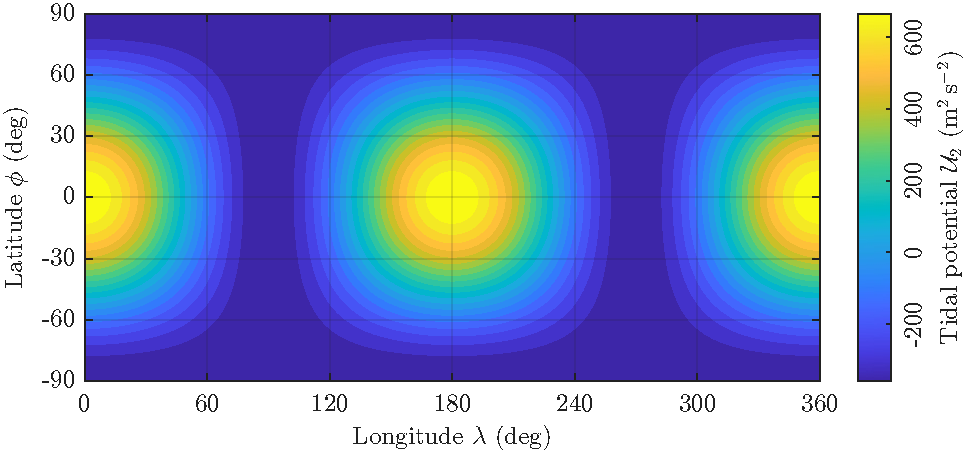
\includegraphics[width=\textwidth]{IMAGES/GANYMEDE_tidal_potential_static.pdf}
        \caption{Permanent part of the tidal potential on Ganymede, computed as the average tidal potential during the GCO.}
        \label{fig:GANYMEDE_tidal_potential}
    \end{subfigure}

    \vspace{0.5cm}

    \begin{subfigure}{\textwidth}
        \centering
        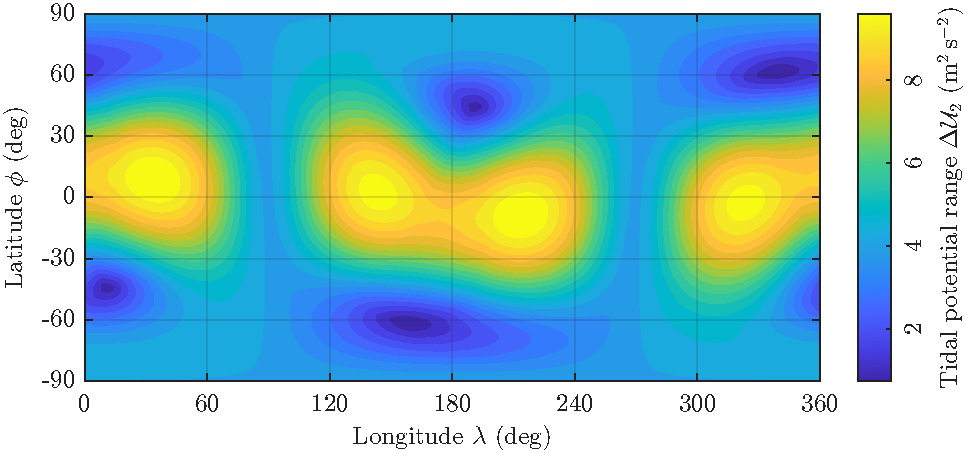
\includegraphics[width=\textwidth]{IMAGES/GANYMEDE_tidal_potential_range.pdf}
        \caption{Maximum variation of the tidal potential due to Jupiter on Ganymede during the GCO.}
        \label{fig:GANYMEDE_tidal_potential_range}
    \end{subfigure}

	  \caption{Tidal potential on Ganymede during the GCO phase. The top panel shows the permanent component of the tidal potential, while the bottom panel shows the maximum variation during the few months of the GCO phase.}
    \label{fig:GANYMEDE_tidal_potential_combined}

\end{figure*}



\subsection{Intermediate test: a controlled DTM corruption}\label{sec:dtm_corruption}

The two configurations considered so far bracket the achievable performance from opposite sides: an identical DTM for generation and fit (recovery to numerical precision, Sect.~\ref{sec:results}), and two independent DTMs whose \SI{26.3}{m} RMS mismatch is realistic but possibly pessimistic, since the two products originate from different instruments and pipelines. To probe the intermediate regime in a controlled way, we use a \emph{single} DTM both for generation and for the fit, but perturb the copy entering the co-registration model $\vec{G}_{\mathrm{LA}}$ by a synthetic, analytically differentiable error field,
%
\begin{align}
	h_{\mathrm{DTM}}^{\mathrm{c}}(\phi, \lambda) &= h_{\mathrm{DTM}}(\phi, \lambda) + \delta h(\phi, \lambda), 
	\\% \qquad
	\delta h(\phi, \lambda) &= \sum_{j=1}^{N} A_j \, \sin\!\left( n_j\, \phi + \alpha_j \right)\cos\!\left( n_j\, \lambda + \beta_j \right),
	\label{eq:corruption_field}
\end{align}
%
with amplitudes $A_j$, integer angular orders $n_j$, and phases $\alpha_j, \beta_j$ drawn uniformly on $[0, 2\pi)$ with a fixed seed. The order $n_j$ sets the number of oscillations over a full revolution, so the characteristic wavelength is $L_{n}=2\pi R_{\mathrm{G}}/n$; restricting $n_j$ to integers keeps $\delta h$ continuous across the $0^\circ/360^\circ$ meridian. Because $\delta h$ is analytic, its slopes $\partial\delta h/\partial\phi$ and $\partial\delta h/\partial\lambda$ are added in closed form to the topographic slopes entering the observation partials $\tilde{\vec H}_i$ of Eq.~\eqref{eq:dGdstate}, so the perturbed surface and the slopes used in the fit remain mutually consistent.

We restrict the perturbation to low orders, $n=1$ and $n=2$, for both physical and methodological reasons. Stereo-photogrammetric DTMs are dominated by long-wavelength, spatially correlated systematic errors -- regional tilts and broad warps from baseline geometry, illumination, and bundle adjustment -- rather than by white short-wavelength noise, which averages out over the $\sim\!10^{7}$ GALA footprints. More importantly, the long-wavelength component is the one geometrically degenerate with the slowly varying orientation of the body, and hence the component most liable to alias into the rotational state and the moments of inertia. Order $n=1$ ($L_1 \approx \SI{16500}{km}$) represents a hemispheric tilt; order $n=2$ ($L_2 \approx \SI{8300}{km}$) a broad doming. We emphasise that Eq.~\eqref{eq:corruption_field} is a controlled parametric perturbation, not a spectral fit to a measured DTM-error field, and that the factors are undulations of angular order $n$, not spherical harmonics.

We adopt $A_1 = \SI{3}{m}$ at $n=1$ and $A_2 = \SI{1}{m}$ at $n=2$, decreasing with order so that the field is dominated by the longest wavelength, giving an area-weighted RMS of $\delta h_{\mathrm{RMS}} = \SI{1.58}{m}$. This is a deliberately conservative error, well below the \SIrange{10}{20}{m} vertical accuracy quoted for stereo DTMs (Sect.~\ref{sec:GALA_data}); as shown below, even at this level the long-wavelength error propagates into the interior parameters, so it provides a sensitive lower bound. The phases are randomised to avoid imprinting an artificial alignment with the body-fixed frame. Because the recovered parameters depend on amplitude and phase, we treat this realisation as one point of a sensitivity analysis, repeated over independent phase draws and over a range of $\delta h_{\mathrm{RMS}}$. % CONFIRM: only if you actually run the sweep/ensemble; otherwise soften to "should be repeated over"


%-----------------------------------------------------------------------
\section{Results}\label{sec:results}
%-----------------------------------------------------------------------

%-----------------------------------------------------------------------
% FIGURE LASER RESIDUALS HISTOGRAM
%-----------------------------------------------------------------------
\begin{figure*}[h]
    \centering
    \begin{overpic}[width=\textwidth]{IMAGES/ganymede_laser_residuals_hist_14_04_26.pdf}
          \put(41,1){%
            % \colorbox{white}{%
            %     \rotatebox{0}{$\vec{y}-\vec{G}_{\mathrm{LA}}\ \mathrm{(m)}$}%
            % }%
        }
    \end{overpic}
    \caption{Histograms of the laser range residuals (observed minus computed) for different iteration of the differential correction.}
    \label{fig:ganymede_laser_residuals_hist}
\end{figure*}

%-----------------------------------------------------------------------
% CORRELATION MATRIX
%-----------------------------------------------------------------------
\begin{figure*}[h]
    \centering
    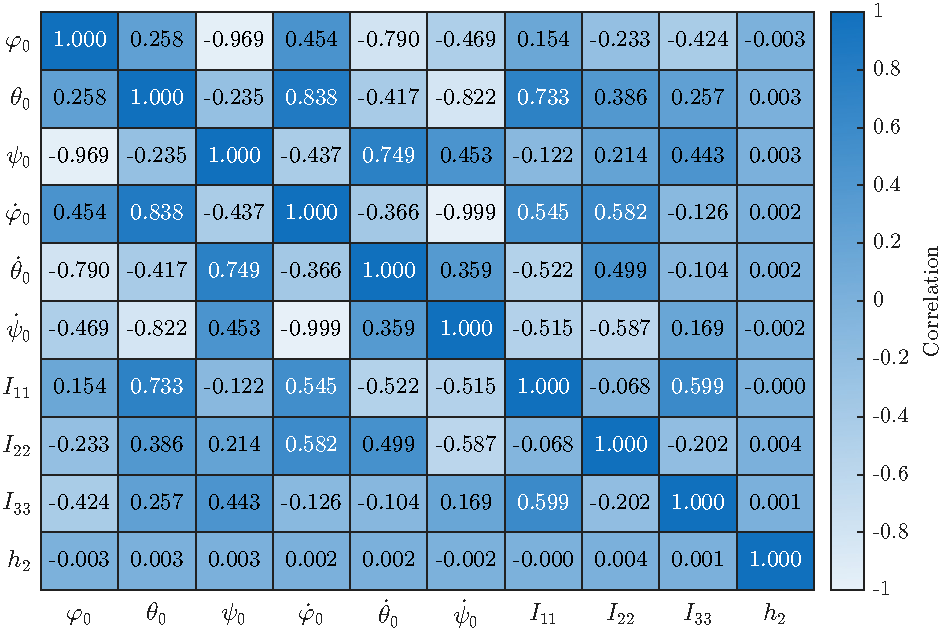
\includegraphics[width=\textwidth]{IMAGES/ganymede_correlation_14_04_26.pdf}
    \caption{Correlation matrix (${\vec{\rho}}$) of the estimated variables at the last iteration.}
    \label{fig:ganymede_correlation_matrix}
\end{figure*}



%-----------------------------------------------------------------------
% STANDARD DEVIATIONS OF ESTIMATED PARAMETERS
%-----------------------------------------------------------------------
\begin{table*}
\centering
\caption{Ground truth values and estimated parameters and associated standard deviations ($\sigma$) in SI units, from the GALA synthetic observations.}
\label{tab:GALA_ground_truth_estimates}
\begin{tabular}{l c c r}
\hline \hline
Parameter & Ground truth & Estimated ($\pm \sigma$) & Unit \\
\hline
% --- rows printed by MATLAB go here ---
% Parameter & True Value & Estimated ($\pm$ $\sigma$) & Units \\ 
$\varphi_0$ & \num{6.24688} & \num{6.24680} $\pm$ \num{5.29e-07} & \unit{rad} \\
 $\theta_0$ & \num{0.44759} & \num{0.44763} $\pm$ \num{1.54e-07} & \unit{rad} \\
  $\psi_0$ & \num{2.89119} & \num{2.89126} $\pm$ \num{5.11e-07} & \unit{rad} \\ 
  $\dot{\varphi}_0$ & \num{-1.55518} & \num{-1.01260} $\pm$ \num{0.02686} & $10^{-10}$ \unit{rad.s^{-1}} \\
   $\dot{\theta}_0$ & \num{-1.43793} & \num{0.23024} $\pm$ \num{0.17137} & $10^{-11}$ \unit{rad.s^{-1}} \\ 
   $\dot{\psi}_0$ & \num{1.01644} & \num{1.01644} $\pm$ \num{0.00000} & $10^{-5}$ \unit{rad.s^{-1}} \\
    $I_{11}$ & \num{9.50641} & \num{10.59483} $\pm$ \num{0.00856} & $10^{34}$ \unit{kg.m^2} \\
	 $I_{22}$ & \num{9.52214} & \num{10.94134} $\pm$ \num{0.02236} & $10^{34}$ \unit{kg.m^2} \\
	  $I_{33}$ & \num{9.52738} & \num{10.52629} $\pm$ \num{0.00699} & $10^{34}$ \unit{kg.m^2} \\ 
	  % $I_{12}$ & \num{0.00000} & -- $\pm$ \num{0.00000} & $10^{34}$ \unit{kg.m^2} \\ 
	  % $I_{13}$ & \num{0.00000} & -- $\pm$ \num{0.00000} & $10^{34}$ \unit{kg.m^2} \\
	   % $I_{23}$ & \num{0.00000} & -- $\pm$ \num{0.00000} & $10^{34}$ \unit{kg.m^2} \\ 
	   % $k_{\mathrm{o}}$ & \num{2.78457} & -- $\pm$ \num{0.00003} & $10^{23}$ \unit{kg.m^2.s^{-1}} \\
	    $h_2$ & \num{1.50000} & \num{1.43499} $\pm$ \num{0.01182} & -- \\
		 \hline $d_\mathrm{s}$ & \num{263.192} & \num{298.715} $\pm$ \num{0.256} & \unit{km} \\
% % Parameter & True Value & Estimated ($\pm$ $\sigma$) & Units \\
% $\phi_0$ & \num{6.24688} & \num{6.24687} $\pm$ \num{2.07e-07} & \unit{rad} \\
% $\theta_0$ & \num{0.44759} & \num{0.44759} $\pm$ \num{6.64e-08} & \unit{rad} \\
% $\psi_0$ & \num{2.89119} & \num{2.89119} $\pm$ \num{1.97e-07} & \unit{rad} \\
% $\dot{\phi}_0$ & \num{-1.55518} & \num{-1.65454} $\pm$ \num{0.01149} & $10^{-10}$ \unit{rad.s^{-1}} \\
% $\dot{\theta}_0$ & \num{-1.43793} & \num{-0.46485} $\pm$ \num{0.06436} & $10^{-11}$ \unit{rad.s^{-1}} \\
% $\dot{\psi}_0$ & \num{1.01644} & \num{1.01644} $\pm$ \num{0.00000} & $10^{-5}$ \unit{rad.s^{-1}} \\
% $I_{11}$ & \num{9.50641} & \num{9.70019} $\pm$ \num{0.01748} & $10^{34}$ \unit{kg.m^2} \\
% $I_{22}$ & \num{9.52214} & \num{9.67854} $\pm$ \num{0.00316} & $10^{34}$ \unit{kg.m^2} \\
% $I_{33}$ & \num{9.52738} & \num{9.64247} $\pm$ \num{0.00250} & $10^{34}$ \unit{kg.m^2} \\
% % $I_{12}$ & \num{0.00000} & -- $\pm$ \num{0.00000} & $10^{34}$ \unit{kg.m^2} \\
% % $I_{13}$ & \num{0.00000} & -- $\pm$ \num{0.00000} & $10^{34}$ \unit{kg.m^2} \\
% % $I_{23}$ & \num{0.00000} & -- $\pm$ \num{0.00000} & $10^{34}$ \unit{kg.m^2} \\
% % $k_{\mathrm{o}}$ & \num{2.78457} & -- $\pm$ \num{0.00003} & $10^{23}$ \unit{kg.m^2.s^{-1}} \\
% $h_2$ & \num{1.50000} & \num{1.48731} $\pm$ \num{0.00543} & -- \\
% \hline
% $d_\mathrm{s}$ & \num{263.192} & \num{267.177} $\pm$ \num{0.087} & \unit{km} \\
% --------------------------------------
\hline
\end{tabular}
\end{table*}



% ------------------------------------------------------------------------------------------------------------------
% -------------------------------------- MAIN TEXT (RESULTS) -------------------------------------------------------
% ------------------------------------------------------------------------------------------------------------------

To test the consistency of the model, we first attempt to recover the ground truth parameters in a test case where the DTM used to generate the synthetic observations is the same as that employed in the differential correction scheme, and no white noise is added to the synthetic observations. We find that the model is able to retrieve the initial conditions, moments and products of inertia, and $h_2$ to numerical precision in only a few iterations. 
This test, however, is of limited use in assessing the capability of the method to recover the relevant parameters in a real world scenario. We therefore test the code in a more realistic configuration.

Table~\ref{tab:GALA_ground_truth_estimates} reports the ground truth values, the estimated parameters, and the corresponding standard deviations $\sigma$ after $n$ iterations. The RMS of the laser measurements residuals (observed minus computed) after the last iteration is approximately 
\SI{7.5}{m}. % see Fig.4 (histogram)
%
%  close to the assumed variance of the noise level, as it should be expected. %since the rms of white noise is sigma.
% Sensitivity is highest for the initial Euler angles and Euler angle rates, followed by the polar moment of inertia $C$ and the Love number $h_2$. The lowest sensitivity is found for the equatorial moments of inertia $A$ and $B$.
% We test the code by starting with several different initial guesses, and it converges every time. ???

Figure~\ref{fig:ganymede_laser_residuals_hist} shows the histograms of the laser range residuals  at different iterations of the differential correction procedure. 
%
% In the same plot we show the difference along the reference solution between the topography of the stereo DTM and that of the DTM from laser altimetry, used to generate the measurements. % We see that the error is basically due only to the stereo


Our observations are simulated with a cadence of one measurement per second, that is \SI{1}{Hz}, in order to reduce the computational cost.
Over the GCO-500 phase, this corresponds to approximately $\num{e7}$ laser measurements. For simplicity, we do not account for possible instrument or operational downtimes, since the accuracy of the parameter retrieval is expected to depend primarily on the total observation time span.
This sampling frequency is significantly lower than the nominal capability of GALA, which will operate at \SI{30}{Hz} \citep{2019Geosc...9..320S}. Nonetheless, our simulations show that even such a low cadence yields promising results.


A joint analysis of the parameter estimates in Table~\ref{tab:GALA_ground_truth_estimates} and the correlation matrix in Fig.~\ref{fig:ganymede_correlation_matrix} provides a comprehensive picture of the estimator's performance and the physical coupling of the system. 
%
Assuming an observation window corresponding to the GCO phase we are able to retrieve the moments of inertia and Euler angles to high precision. Under these conditions, the ground truth thickness of the icy shell, set at one-tenth of Ganymede's reference radius (\SI{263.1}{km}), is recovered as 
${d_{\mathrm{s}} = \SI{298.71 \pm 0.26}{km}}$.
% 
However, we note that these results are strongly dependent on the noise level in the measurements, as well as on orbit reconstruction and pointing errors. In particular, with a higher uncertainty level in the orbit, the filter struggles to properly separate the $I_{22}$ and $I_{33}$ moments, resulting in a significantly higher correlation.
%
% ${\sigma_{\mathrm{LA}} = \SI{10}{m}}$
% significantly degrades this precision, expanding the uncertainty of the estimated shell thickness to approximately $\pm\SI{30}{km}$.
%
The tidal Love number is estimated at
${h_2 = \num{1.434} \pm \num{0.012}}$, close to the ground truth value of $\num{1.5}$, close to the $3\sigma$ formal uncertainty. As revealed by the correlation matrix, this success is driven by the fact that $h_2$ is fundamentally decoupled from the rest of the state vector, exhibiting correlation coefficients smaller than $0.01$. Consequently, the tidal deformation signal can be robustly separated from both the static gravity field and the rotational dynamics.
%
Conversely, a critical examination of the principal moments of inertia ($I_{11}$, $I_{22}$, and $I_{33}$) reveals that their formal $1\sigma$ uncertainties underestimate the true estimation error. For instance, the estimated $I_{22}$ deviates from the ground truth by approximately 
$\SI{0.14e34}{kg.m^2}$, an offset far exceeding its formal standard deviation of 
$\SI{0.00465e34}{kg.m^2}$. 
%
% This bias is fully explained by the extreme positive correlations observed in Fig.~\ref{fig:ganymede_correlation_matrix}, which reach $0.997$ between $I_{11}$ and $I_{33}$, and 
% $0.933$ between $I_{11}$ and $I_{22}$. 

Furthermore, the kinematic parameter recovery highlights the inherent limits of formal covariance analysis in the presence of unmodeled topographic noise. While the primary spin rate $\dot{\psi}_0$ and the initial Euler angles ($\phi_0, \theta_0, \psi_0$) are recovered essentially to numerical precision, the Euler angle rates exhibit some degradation. Specifically, the estimated nutation rate $\dot{\theta}_0$ converged to 
$\SI{-4.65(6)e-12}{rad.s^{-1}}$
against a true value of 
$\SI{-1.438e-11}{rad.s^{-1}}$, despite claiming a highly constrained formal variance. This discrepancy reflects the profound difficulty of isolating small-amplitude kinematic signatures when accounting for pointing and orbit reconstruction errors. This challenge is further echoed in the strong geodetic correlations among the kinematic parameters themselves, notably the 
$-0.885$ anti-correlation between the initial precession angle $\phi_0$ and the proper rotation angle $\psi_0$. 




%% TENTATIVE ALIGNMENT
% \begin{table}
% \centering
% \caption{Ground truth values and estimated parameters with mixed alignment.}
% \label{tab:GALA_ground_truth_estimates}
% \begin{tabular}{
%     c 
%     S[table-format=-1.5e2] 
%     S[table-format=-1.5e2] 
%     S[table-format=1.3e2] 
%     c
% }
% \hline \hline
% {Parameter} & \multicolumn{1}{c}{Ground truth} & \multicolumn{1}{c}{Estimated} & \multicolumn{1}{c}{$\sigma$} & {Unit} \\
% \hline
% % --- ROWS 1-3: Forced Centering using multicolumn ---
% $\phi_0$   & \multicolumn{1}{c}{\num{6.24386}} & \multicolumn{1}{c}{\num{6.24369}} & \multicolumn{1}{c}{\num{7.350e-07}} & \unit{rad} \\
% $\theta_0$ & \multicolumn{1}{c}{\num{0.44769}} & \multicolumn{1}{c}{\num{0.44767}} & \multicolumn{1}{c}{\num{2.585e-07}} & \unit{rad} \\
% $\psi_0$   & \multicolumn{1}{c}{\num{3.69967}} & \multicolumn{1}{c}{\num{3.69984}} & \multicolumn{1}{c}{\num{7.207e-07}} & \unit{rad} \\

% % --- ROWS 4-9: Standard Alignment (S column handles these) ---
% $\dot{\phi}_0$   & -1.25954e-10 & -8.01279e-10 & 5.187e-12 & \unit{rad.s^{-1}} \\
% $\dot{\theta}_0$ & 1.41930e-11  & 7.86523e-10  & 2.806e-12 & \unit{rad.s^{-1}} \\
% $\dot{\psi}_0$   & 1.01646e-05  & 1.01652e-05  & 4.642e-12 & \unit{rad.s^{-1}} \\
% $I_{11}$         & 3.19796e+35  & 3.20819e+35  & 2.883e+32 & \unit{kg.m^2} \\
% $I_{22}$         & 3.19953e+35  & 3.34250e+35  & 2.784e+32 & \unit{kg.m^2} \\
% $I_{33}$         & 3.20006e+35  & 3.27344e+35  & 2.867e+32 & \unit{kg.m^2} \\

% % --- LAST ROW: Forced Centering ---
% $h_2$      & \multicolumn{1}{c}{\num{1.50000}} & \multicolumn{1}{c}{\num{1.39601}} & \multicolumn{1}{c}{\num{2.642e-02}} & -- \\
% \hline
% \end{tabular}
% \end{table}



%-----------------------------------------------------------------------
% FIGURE LASER FOOTPRINTS RESIDUALS
%-----------------------------------------------------------------------
% \begin{figure}[h]
%     \centering
%     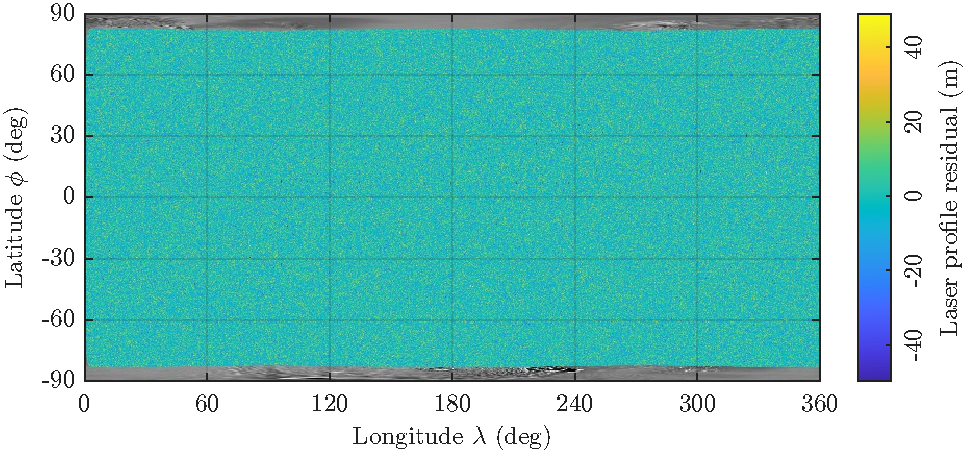
\includegraphics[width=\textwidth]{IMAGES/ganymede_laser_residuals_footprints.pdf}
%     \caption{GALA laser footprints residuals during the GCO.}
% 	% from May 22 2035 (red marker) to September 28 2035 (blue marker).
%     \label{fig:gala_laser_residuals_footprints}
% \end{figure}


% %-----------------------------------------------------------------------
% % FIGURE LASER RESIDUALS (as function of time)
% %-----------------------------------------------------------------------
% \begin{figure}[h]
%     \centering
%     \begin{overpic}[width=\textwidth]{IMAGES/ganymede_laser_residuals_time.pdf}
%           \put(0,30){%
%             \colorbox{white}{%
%                 \rotatebox{90}{$\boldsymbol{y}-\boldsymbol{G}_{\mathrm{LA}}\ \mathrm{(m)}$}%
%             }%
%         }
%     \end{overpic}
%     \caption{Laser range residuals (observed minus computed) for different iteration of the differential correction as a function of time ($t$) in days.}
%     \label{fig:ganymede_laser_residuals}
% \end{figure}



% %_____________________________________________________________
% % FIGURE 3: Ganymede - librational parameters + obliquity and inclination
% %_____________________________________________________________
% \begin{figure}
% 	\centering
% 	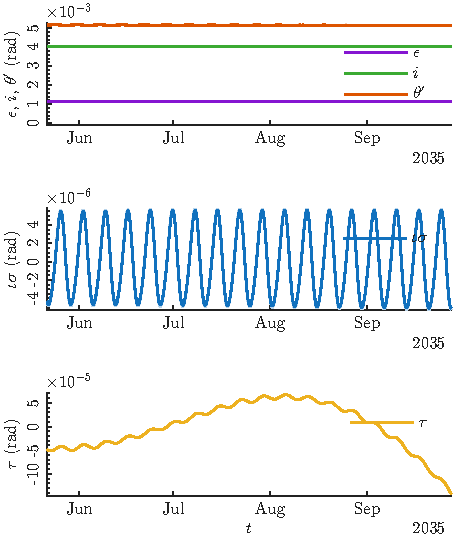
\includegraphics[width=0.8\textwidth]{IMAGES/ganymede_lib_tile_MAY2035_SEP2035.pdf}
% 	\caption{Evolution of the obliquity ($\epsilon$) in purple, orbital inclination ($i$) relative to the Laplace plane in green, and the libration parameters $\iota\sigma$ in blue, $\tau$ in yellow, and $\theta^\prime = \iota + \rho$ in red, for Ganymede during the GCO.}
% 	\label{fig:ganymede_lib_tile_MAY2035_SEP2035}
% \end{figure}


% %_____________________________________________________________
% %FIGURE: POLAR PLOTS
% %_____________________________________________________________
% \begin{figure*}
%     \centering

% 	\begin{subfigure}[t]{0.45\textwidth}
%         \centering
%         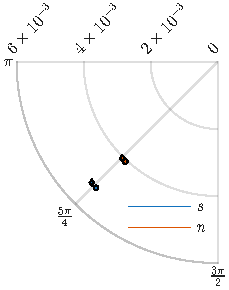
\includegraphics[width=\textwidth]{IMAGES/ganymede_snk_MAR2035_OCT2035.pdf}
%         % \caption{Ganymede}
%         \label{fig:ganymede_snk_MAY2035_SEP2035}
%     \end{subfigure}

%     \caption{Projection of spin axis ${\vec{\omega}}$ (blue) and orbit normal ${\vec{n}}$ (red) of Ganymede on its Laplace plane  ($\mathcal{P}$ horizontal plane), defined by ${\vec{p}}$, for different values of the shell thickness $d_{\mathrm{s}}$. Units are in radians.
% 	Circle markers indicate the initial time at May $15^{\mathrm{th}}$ 2035, while a diamond marker denotes the final time September $28^{\mathrm{th}}$ 2035. The precession is retrograde relative to the orbital revolution and rotation.}
%     \label{fig:galilean_snk_ocean_MAY2035_SEP2035}
% \end{figure*}



\subsection{Recovery with a corrupted DTM}\label{sec:results_corrupted_dtm}

We apply the differential correction to observations generated and fitted with the common DTM of Sect.~\ref{sec:dtm_corruption}, with the fit copy perturbed by the field of Eq.~\eqref{eq:corruption_field}. The behaviour of the estimator separates sharply into a well-determined part and an unidentifiable part, and this separation -- rather than any single recovered value -- is the main result of the test. Representative converged values are listed in Table~\ref{tab:corrupted_dtm_estimates}.

The initial Euler angles $(\phi_0,\theta_0,\psi_0)$ and the spin rate $\dot\psi_0$ are recovered essentially to the precision of the noise-free case. The intermediate and polar moments $I_{22}$ and $I_{33}$ converge to stable values, but biased high by about \SI{5}{\percent} ($\sim\!\SI{0.45e34}{kg.m^2}$), an offset that exceeds their formal $1\sigma$ uncertainties (a few $\times 10^{30}\,\mathrm{kg\,m^2}$) by two to three orders of magnitude. Consequently the inferred ice-shell thickness from Eq.~\eqref{eq:ice_shell_thickness} is ${d_{\mathrm{s}} \approx \SI{279}{km}}$, % CONFIRM
biased by about \SI{16}{km} from the ground-truth \SI{263.2}{km}. This bias is smaller than the $\sim\!\SI{35}{km}$ of the two-DTM case (Table~\ref{tab:GALA_ground_truth_estimates}), confirming the intended intermediate character of the test; that a long-wavelength error of only \SI{1.58}{m} RMS already biases $d_{\mathrm{s}}$ by more than \SI{15}{km} underscores how efficiently long-wavelength DTM error aliases into the interior estimate.

The minimum moment $I_{11}$, by contrast, does not converge. After the other parameters stabilise (near the eighth iteration) its estimate drifts and then diverges across subsequent iterations, swinging over more than an order of magnitude while the observation-residual RMS remains flat at $\approx\!\SI{9.4}{m}$. The normal-equation system is numerically rank-deficient throughout the inversion ($\mathrm{RCOND}\sim 10^{-22}$), with $I_{11}$ identified as the near-singular direction: both its formal and consider standard deviations grow without bound, the latter exceeding the a priori by many orders of magnitude. We therefore report $I_{11}$ as unconstrained rather than as an estimate. The corresponding ratio $A_{\mathrm{s}}/C_{\mathrm{s}}$ wanders in lock-step with $I_{11}$, so the minimum-inertia axis is the unobservable degree of freedom of the rotational fit; we examine why in Sect.~\ref{sec:identifiability}.

\begin{table}[h!]
\centering
\caption{Representative converged parameters for the corrupted-DTM test of Sect.~\ref{sec:dtm_corruption}. The minimum moment $I_{11}$ does not converge and is reported as unconstrained (see text); the $h_2$ value is provisional pending the phase-ensemble analysis of Sect.~\ref{sec:identifiability}.}
\label{tab:corrupted_dtm_estimates}
\begin{tabular}{l c c r}
\hline \hline
Parameter & Ground truth & Estimated & Unit \\
\hline
$\phi_0$        & \num{6.24688} & \num{6.24688} & \unit{rad} \\
$\theta_0$      & \num{0.44759} & \num{0.44762} & \unit{rad} \\
$\psi_0$        & \num{2.89119} & \num{2.89119} & \unit{rad} \\
$\dot{\psi}_0$  & \num{1.01644} & \num{1.01644} & $10^{-5}$ \unit{rad.s^{-1}} \\
$I_{11}$        & \num{9.51}    & \multicolumn{1}{c}{unconstrained} & $10^{34}$ \unit{kg.m^2} \\
$I_{22}$        & \num{9.52}    & \num{9.99}    & $10^{34}$ \unit{kg.m^2} \\
$I_{33}$        & \num{9.53}    & \num{9.98}    & $10^{34}$ \unit{kg.m^2} \\
$h_2$           & \num{1.500}   & \num{1.34}    & -- \\ % CONFIRM (provisional)
\hline $d_\mathrm{s}$ & \num{263.2} & \num{279} & \unit{km} \\ % CONFIRM
\hline \hline
\end{tabular}
\end{table}


\subsection{Identifiability of the moments and consequences for the parameterisation}\label{sec:identifiability}

The divergence of $I_{11}$ is not a numerical accident but a direct manifestation of the near-degeneracy discussed in Sect.~\ref{sec:rotational_eqs_V2}. In the rigid-body limit the rotational equations are invariant under a global rescaling of the inertia tensor (Eq.~\ref{eq:geodesic_explicit_V2}) and depend only on the ratios $\alpha$, $\beta$, $\gamma$. Treating the quadrupole coefficients in the McCullagh potential as injected constants formally breaks this invariance and, in principle, restores sensitivity to the absolute scale. In practice, however, the present test shows that this sensitivity is too weak to constrain the minimum moment from GCO altimetry: the rotational signal depends only marginally on $A_{\mathrm{s}} = I_{11}$, the long axis pointing toward Jupiter, and the normal equations are correspondingly singular in that direction ($\mathrm{RCOND}\sim 10^{-22}$). The well-determined combinations are the polar moment $C_{\mathrm{s}} = I_{33}$ -- and hence $d_{\mathrm{s}}$ -- together with $I_{22}$, while $I_{11}$ remains effectively unobservable. This qualifies the statement of Sect.~\ref{sec:rotational_eqs_V2}: injecting the gravity field permits estimation of the well-observed moments, but does not by itself render all three principal moments independently recoverable from altimetry.

The remedy is to stop solving for the minimum moment as a free absolute parameter and instead to fix it through the gravity field, which is exactly the information the 3GM experiment is expected to provide. Since the injected coefficient $C_{22}$ is related to the equatorial moments by Eq.~\eqref{eq:inertia2stokes_V2_C22_V2}, the minimum moment follows from the well-determined $I_{22}$ as $I_{11} = I_{22} - 4 {M}_{\mathrm{G}} R_{\mathrm{G}}^2\, C_{22}$, removing the singular direction from the solve-for set. Equivalently, the estimation can be reparametrized in terms of the ratios $\alpha$, $\beta$, $\gamma$ and $h_2$, with the absolute scale supplied externally by $C_{20}$ and $C_{22}$. Either choice eliminates the unconstrained direction that causes the $I_{11}$ divergence while retaining the quantities the altimetry actually determines, and we adopt it as the recommended estimation strategy.

A practical corollary concerns the convergence criterion. Monitoring only the observation-residual RMS (Sect.~\ref{sec:DC_laser}) is insufficient when a parameter is weakly observable: the residual RMS is by construction nearly flat along the unobservable direction, so the iteration can appear converged on the RMS metric while $I_{11}$ continues to drift. We therefore also monitor the norm of the parameter increment $\|\delta\tilde{\vec x}_0\|$ and terminate only when both metrics fall below tolerance.


A further feature of this realisation is that $h_2$ converges to $\approx\!\num{1.34}$, % CONFIRM
i.e. biased low by about \SI{11}{\percent} -- further from the ground truth than in the two-DTM case, despite the milder DTM error. Because the $n=2$ corruption term shares the angular order of the degree-two tidal deformation, we suspected a spectral overlap between the long-wavelength DTM error and the tidal signal. To test this we repeated the inversion over an ensemble of independent corruption phases at fixed amplitude.
% BRANCH A (ensemble shows scatter -> phase artifact):
% The recovered h_2 varies by ~X across realisations, indicating that the apparent bias is a feature of the particular phase pattern rather than a systematic effect; the ensemble mean is h_2 = <..> +/- <..>, consistent with the decoupling found in Sect.~\ref{sec:results}.
% BRANCH B (ensemble stable -> real overlap):
% The recovered h_2 remains biased low across all realisations, confirming a genuine degeneracy between order-two DTM error and the tidal deformation. This identifies a specific failure mode for h_2 recovery: long-wavelength DTM error of the same angular order as the tide aliases directly into the tidal channel, and must be controlled (e.g. by crossover-based separation) in the analysis of real GALA data.

\section{Conclusions}\label{sec:conclusions}

We have presented a fully dynamical framework for estimating the rotational state, the principal moments of inertia, and the tidal Love number $h_2$ of Ganymede from laser altimetry. In contrast to kinematic profile fitting, the satellite orientation is propagated through the tri-axial second-order Euler-angle equations derived from a Lagrangian formulation; the quadrupole gravity coefficients are injected as independent constants so as to break the scale invariance of the rigid-body equations; and the mechanical decoupling induced by a subsurface ocean is represented through a laminar shell--ocean coupling described by a Rayleigh dissipation function. The reliability of the solution and the correlations among the parameters are assessed through a consider-covariance analysis, and the method is exercised on synthetic GALA observations spanning the GCO phase, with realistic instrument noise, pointing errors, and orbit-reconstruction errors.

The estimation results separate cleanly into a well-observed part and a poorly observed part. The tidal Love number is the most robustly determined parameter: it is essentially decoupled from the rest of the state vector, with correlation coefficients below $0.01$, so the tidal-deformation signal can be isolated from both the static gravity field and the rotational dynamics. Its formal precision is competitive with the crossover-based estimate of \citet{2015P&SS..117..184S}, although, as for the moments of inertia, its accuracy is ultimately limited by systematic DTM and pointing errors rather than by the formal covariance. The initial Euler angles and the spin rate $\dot{\psi}_0$ are likewise recovered to high accuracy, whereas the slow nutation and precession rates are markedly more sensitive to the unmodelled errors. The principal moments of inertia are recovered with systematic biases that exceed their formal $1\sigma$ uncertainties, so the formal covariance substantially underestimates the true error in the presence of unmodelled topographic signal and correlated orbit errors.

The most important limitation we identify concerns the absolute moments of inertia. Although injecting the gravity coefficients formally restores sensitivity to the absolute scale, our experiments show that the minimum principal moment $A_{\mathrm{s}} = I_{11}$, associated with the long axis pointing toward Jupiter, remains effectively unobservable from GCO altimetry: it is the near-singular direction of the normal equations ($\mathrm{RCOND}\sim 10^{-22}$), it fails to converge, and both its formal and consider uncertainties diverge. The well-determined quantities are instead the polar moment $C_{\mathrm{s}} = I_{33}$ -- and hence the ice-shell thickness -- together with the intermediate moment $I_{22}$. This qualifies the notion that the injection alone renders all three principal moments independently recoverable, and points to a concrete remedy: the minimum moment should be fixed through the gravity field, via the relation $I_{11} = I_{22} - 4 {M}_{\mathrm{G}} R_{\mathrm{G}}^2\,C_{22}$, or, equivalently, the estimation should be reparameterised in terms of the moment ratios and $h_2$, with the absolute scale supplied by $C_{20}$ and $C_{22}$. Either choice removes the unconstrained direction while retaining the quantities the altimetry actually determines, and we adopt it as the recommended estimation strategy for the JUICE data.

A controlled, long-wavelength corruption of the digital terrain model confirms this picture from the data side and quantifies the sensitivity of the method to topographic error. Using a single DTM for both the generation and the fit, with the fit copy perturbed by an analytic field dominated by the lowest angular orders, we find that even a perturbation of \SI{1.58}{m} RMS biases the inferred ice-shell thickness by more than \SI{15}{km} -- smaller than the $\sim\!\SI{35}{km}$ bias obtained with two independent DTMs, and thus intermediate between the noise-free and the fully mismatched configurations, as intended. The efficiency with which such a small, long-wavelength error propagates into the interior estimate underscores that the dominant threat to the recovery is not the high-frequency measurement noise, which averages down over the $\sim\!10^{7}$ footprints, but the long-wavelength, spatially correlated component of the DTM error, which is geometrically degenerate with the slowly varying orientation of the body.

Taken together, these results indicate that GCO laser altimetry provides a strong, independent constraint on the tidal Love number, and hence on the presence of a subsurface ocean, but does not by itself separate the individual absolute moments of inertia. The method is therefore best regarded as complementary to the 3GM radio-science experiment and to crossover analyses, with which it should be combined. Future work should replace the reference-sphere footprint with an iterative intersection on the actual DTM surface, integrate the ocean-layer Euler angles self-consistently rather than prescribing them, propagate the JANUS-derived DTM and its error budget once available, and assess a joint inversion of altimetry, gravity, and crossovers. A systematic characterisation of the achievable accuracy as a function of the amplitude and spectral content of the DTM error, building on the controlled corruption introduced here, will be an essential ingredient of that assessment.


%-----------------------------------------------------------------------
%---------- APPENDICES -------------------------------------------------
% \begin{subappendices} % comment SN
\begin{appendices}    % uncomment SN
%-----------------------------------------------------------------------


%_____________________________________________________________
\section{Rotation matrices and Euler angles} \label{appendix:rotm_V2}
%_____________________________________________________________
% see: https://mathworld.wolfram.com/EulerAngles.html




% The estimated initial conditions for the Galilean satellites at the J2000.0 epoch, in the ICRF frame ($\mathcal{I}$) are given in Table~\ref{tab:euler_initial_conditions}.

%The frames are right-handed of course, write it somewhere.
The Euler angles in the 3-1-3 order define the three successive rotations that orient the body-fixed frame $\mathcal{B}$ relative to the inertial frame $\mathcal{I}$ axes.
\citep[see, e.g.,][]{Broucke1990doi:10.2514/3.20591}.
The right-handed proper rotation matrix 
${\vec{R}_{\mathcal{B}}^{\mathcal{I}} = \vec{R}(\varphi,\theta,\psi)}$.
%
The rotation can be decomposed into the three successive rotation as
\begin{align}
\vec{R}_{\mathcal{B}}^{\mathcal{I}}= 
\vec{R}_{z}(\psi)
\vec{R}_{x}(\theta)
\vec{R}_{z}(\varphi)
= \vec{R}(\varphi,\theta,\psi)
	% \\= \begin{pmatrix}
	% \cos\psi \cos\varphi - \sin\psi \cos\theta \sin\varphi &
	% \cos\psi \sin\varphi + \sin\psi \cos\theta \cos\varphi &
	% \sin\psi \sin\theta \\
	% %
	% -\sin\psi \cos\varphi - \cos\psi \cos\theta \sin\varphi &
	% -\sin\psi \sin\varphi + \cos\psi \cos\theta \cos\varphi &
	% \cos\psi \sin\theta \\
	% %
	% \sin\theta \sin\varphi &
	% -\sin\theta \cos\varphi &
	% \cos\theta
	% \end{pmatrix},
\end{align}
%
where we defined
%
\begin{align}
	\vec{R}_{z}(\psi) &= 
\begin{pmatrix}
	\cos\psi & \sin\psi & 0 \\
	-\sin\psi & \cos\psi & 0 \\
	0 & 0 & 1
\end{pmatrix}, \\ % \quad
\vec{R}_{x}(\theta) & =
	\begin{pmatrix}
1 & 0 & 0 \\
0 & \cos\theta & \sin\theta \\
0 & -\sin\theta & \cos\theta
\end{pmatrix}, \\ %\quad
\vec{R}_{z}(\varphi) & =
	\begin{pmatrix}
\cos\varphi & \sin\varphi & 0 \\
-\sin\varphi & \cos\varphi & 0 \\
0 & 0 & 1
\end{pmatrix}.
% \vec{R}_{y}(\alpha) & =
%  \begin{pmatrix}
% \cos\alpha & 0 & -\sin\alpha  \\
% 0 & 1 & 0  \\
% \sin\alpha & 1 & \cos\alpha
% \end{pmatrix}.
\end{align}
%


Since rotation matrices are orthogonal, the inverse rotation is obtained by simple transposition, that is, ${\vec{R}^{-1} = \vec{R}^\top}$, and it holds
\begin{equation}
	\vec{R}_{\mathcal{I}}^{\mathcal{B}} =
	%\left(\vec{R}_{\mathcal{B}}^{\mathcal{I}}\right)^{-1} =
	%\left(\vec{R}_{\mathcal{B}}^{\mathcal{I}}\right)^\top
	%= \vec{R}^\top.
	\vec{R}^\top = 	\vec{R}_{z}(-\varphi)
	\vec{R}_{x}(-\theta)
	\vec{R}_{z}(-\psi)
	= \vec{R}(-\psi,-\theta,-\varphi).
	\end{equation}
%
Then, the coordinates of a vector in the body frame $ \vec{r}_\mathcal{B}$ are transformed in inertial coordinates $ \vec{r}_\mathcal{I}$  as
%
\begin{equation}
	\label{eq:vecB2I_V2}
%  \vec{r}_\mathcal{B} =
%   \vec{R}_{\mathcal{B}}^{\mathcal{I}}(\varphi,\theta,\psi) 
%   \vec{r}_\mathcal{I}.
\vec{r}_\mathcal{I} =
\vec{R}_{\mathcal{I}}^{\mathcal{B}} %(\varphi,\theta,\psi)
%   \vec{r}_\mathcal{B} =
%\vec{R}^\top 
\vec{r}_\mathcal{B}.
\end{equation}
%
Explicitly the components of $\vec{R}(\varphi,\theta,\psi) = (R_{ij})$ are
%
% \begin{subequations}
\begin{align}
R_{11} &= \cos\psi \cos\varphi - \sin\psi \cos\theta \sin\varphi, \nonumber\\ \displaybreak[2]
R_{12} &= \cos\psi \sin\varphi + \sin\psi \cos\theta \cos\varphi, \nonumber\\ \displaybreak[2]
R_{13} &= \sin\theta \sin\psi , \nonumber\\ \displaybreak[2]
R_{21} &= -\sin\psi \cos\varphi - \cos\psi \cos\theta \sin\varphi, \nonumber\\ \displaybreak[2]
R_{22} &= -\sin\psi \sin\varphi + \cos\psi \cos\theta \cos\varphi, \nonumber\\ \displaybreak[2]
R_{23} &= \sin\theta \cos\psi , \nonumber\\ \displaybreak[2]
R_{31} &= \sin\theta \sin\varphi, \nonumber\\ \displaybreak[2]
R_{32} &= -\sin\theta \cos\varphi, \nonumber\\ \displaybreak[2]
R_{33} &= \cos\theta.
\end{align}
% \end{subequations}

This rotation matrices correspond to  counterclockwise rotations of the about the respective intermediate axes.
In particular $\varphi$ is the angle between the $\vec{e}_{1,\mathcal{I}}$ axis and the ascending node of the satellite equator, $\theta$ is the inclination of the satellite equator to the inertial frame equator, and $\psi$ is the angle between the ascending node and the satellite's prime meridian, that is the $\vec{e}_{1,\mathcal{B}}$ axis \citep{2018CeMDA.130...22A}.

%${\theta \neq 0, \pi}$
If ${\sin\theta \neq 0}$, there are two distinct sets of angles, modulo $2\pi$,  that yield the same rotation matrix. Indeed, one can easily verify that 
\begin{equation}
\vec{R}(\varphi,\theta,\psi) = \vec{R}(\varphi + \pi,-\theta,\psi + \pi).
\end{equation} 
%
If we seek the set such that ${\theta >0}$, then the Euler angles,  modulo $2\pi$, can be retrieved from the components ($R_{ij}$) of the rotation matrix, using the two argument arctangent, as
\begin{align}
	\varphi &= \atantwo(R_{31}, -R_{32}), \notag\\
	\theta &= \acos \left( R_{33} \right), \\
	\psi &= \atantwo(R_{13}, R_{23}). \notag
\end{align}
% \begin{align}
% 	\varphi &= \atan \frac{R_{31}}{-R_{32}}, \quad 
% 	%move the - sign out of atan?
% 	\theta = \acos R_{33}, \quad
% 	\psi = \atan \frac{R_{13}}{R_{23}}.
% % \end{align}


% The rotation that orients the principal axes frame $\mathcal{B}$ in the Laplace frame $\mathcal{P}$ to can be written as
% \begin{equation}
% 	\vec{R}^{\mathcal{P}}_{\mathcal{B}} =
% 	\vec{R}^{\mathcal{P}}_{\mathcal{I}} 
% 	\vec{R}_{\mathcal{B}}^{\mathcal{I}} = 
%  	\vec{R}_{z}({\psi^\prime})
% 	\vec{R}_{x}(\theta^\prime)
% 	\vec{R}_{z}(\varphi^\prime)
% 	= \vec{R}({\varphi^\prime},{\theta^\prime},{\psi^\prime}),
% \end{equation}
% %
% The static rotation matrix  $\vec{R}^{\mathcal{P}}_{\mathcal{I}}$  that transforms the coordinates of a vector expressed in the $\mathcal{P}$ frame into coordinates in the $\mathcal{I}$ frame is the matrix whose columns are the basis vectors of $\mathcal{P}$ expressed in the $\mathcal{I}$ frame.

% The coordinates of the Galilean satellites' respective Laplace poles, expressed in the inertial frame, are given in Table~\ref{tab:laplace_pole_in_ICRF}, where ${\vec{p}_\mathcal{I} = (p_1, p_2, p_3)^\top}$ denotes the unit vector of the Laplace pole in the ICRF ($\mathcal{I}$).



% Then, the transformation from the body-fixed coordinates to the Laplace frame coordinates can be written as
% \begin{equation}
% 	\vec{r}_\mathcal{P} =
% 	\vec{R}_{\mathcal{P}}^{\mathcal{B}}\vec{r}_\mathcal{B} = 
% 	\vec{R}(-{\psi^\prime},-{\theta^\prime}, -{\varphi^\prime})
% 	\vec{r}_\mathcal{B}.
% \end{equation}
% %we can write 
% ${\vec{R}_{\mathcal{B}}^{\mathcal{P}} = \vec{R}(\varphi^\prime, \theta^\prime, \psi^\prime)}$
%%%

% \begin{equation}
% 	\vec{R}^{\mathcal{I}}_{\mathcal{P}}
% 	= 	\vec{R}_{z}(\tilde{\psi})
% 	\vec{R}_{x}(\tilde{\theta})
% 	\vec{R}_{z}(\tilde{\varphi}) = 
% 	\vec{R}(\tilde{\varphi},\tilde{\theta},\tilde{\psi}),
% \end{equation}
% %
%where ${(\tilde{\varphi},\tilde{\theta},\tilde{\psi}})$ are the constant 3-1-3 Euler angles that parametrize the static transformation. 
%The inverse of this transformation is obtained as usual by transposition, since rotation  matrices are orthogonal.


For further details about rotations and Euler angles the reader is referred to \citet{Goldstein:102554} and \citet{LANDAU1976}.




%--------------------------------------------------------------------------------------------
%----------------- RMS --------------------------------- ------------------------------------
%--------------------------------------------------------------------------------------------
% \section{Root mean squared error}

% % The weighted root mean square error (RMS) of the pre-fit observation residuals can be computed as:
% % %
% % \begin{equation}
% %     \label{eq:RMS_weighted}
% %     \mathrm{RMS}_{\mathrm{w}}
% %     =
% %     \sqrt{\frac{\sum_{i=1}^{l}\delta{y}_i^\top \vec{W}_i \delta{y}_i}{\sum_{i=1}^{l} \mathrm{tr}(\vec{W}_i)}}.
% % \end{equation}

% The root mean square error (RMS) of the observation residuals generally is computed and may be used as a measure of convergence; when the RMS no longer changes, within some given tolerance, the solution is assumed to have converged.
% The unweighted RMS can be computed as
% %
% \begin{equation}
% 	\label{eq:RMS}
% 	\mathrm{RMS}
% 	=
% 	\sqrt{\frac{1}{l}\sum_{i=1}^{l}\delta{y}_i^\top \delta{y}_i},
% \end{equation}



% The best estimate of the observation error after the correction of the parameters is given by
% \begin{align}
% 	\hat{\varepsilon}_i &= \delta{y}_i - \vec{H}_i \delta\tilde{\vec{x}}_0, \label{eq:22.73}
% \end{align}
% %
% Then the predicted weighted RMS is computed from
% \begin{equation}
% 	\widehat{\mathrm{RMS}}_{\mathrm{w}} = \sqrt{\frac{1}{l}\displaystyle\sum_{i=1}^{l} \hat{\varepsilon}_i^\top 
% 	\vec{W}_i%R^{-1}
% 	\hat{\varepsilon}_i}. \label{eq:rms_def} %k = l!! p = 1
% \end{equation}
% %
% where $l$ is the number of processed observations. To compute this statistic efficiently without storing the history of all residuals $\hat{\varepsilon}_i$ and measurement matrices $\vec{H}_i$ (which requires excessive memory), we expand the quadratic term. Recalling that the post-fit residual is defined as $\hat{\varepsilon}_i = \delta{y}_i - \vec{H}_i \delta\tilde{\vec{x}}_0$, the weighted sum of squares can be written as:
% % \begin{align}
% % 	\nonumber
% % 	\displaystyle\sum_{i=1}^{l} \hat{\varepsilon}_i^\top 
% % 	\vec{W}_i
% % 	\hat{\varepsilon}_i 
% % 	% 
% % 	&= \sum_{i=1}^{l} (\delta{y}_i - \vec{H}_i \delta\tilde{\vec{x}}_0)^\top \vec{W}_i (\delta{y}_i - \vec{H}_i \delta\tilde{\vec{x}}_0) 
% % 	\\
% % 	&= \sum_{i=1}^{l} \left( \delta{y}_i^\top \vec{W}_i \delta{y}_i - \delta{y}_i^\top \vec{W}_i \vec{H}_i \delta\tilde{\vec{x}}_0 - \delta\tilde{\vec{x}}_0^\top \vec{H}_i^\top \vec{W}_i \delta{y}_i + \delta\tilde{\vec{x}}_0^\top \vec{H}_i^\top \vec{W}_i \vec{H}_i \delta\tilde{\vec{x}}_0 \right).
% % \end{align}
% % Since the term $\delta{y}_i^\top \vec{W}_i \vec{H}_i \delta\tilde{\vec{x}}_0$ is a scalar, it is equal to its transpose $\delta\tilde{\vec{x}}_0^\top \vec{H}_i^\top \vec{W}_i \delta{y}_i$. We can thus group the terms and distribute the summation:
% \begin{align}
% 	\displaystyle\sum_{i=1}^{l} \hat{\varepsilon}_i^\top 
% 	\vec{W}_i
% 	\hat{\varepsilon}_i 
% 	%
% 	&= \sum_{i=1}^{l} \delta{y}_i^\top \vec{W}_i \delta{y}_i
% 	- 2 \delta\tilde{\vec{x}}_0^\top \left( \sum_{i=1}^{l} \vec{H}_i^\top \vec{W}_i \delta{y}_i \right) 
% 	\nonumber \\ 
% 	& \quad +
% 	\delta\tilde{\vec{x}}_0^\top \left( \sum_{i=1}^{l} \vec{H}_i^\top \vec{W}_i \vec{H}_i \right) \delta\tilde{\vec{x}}_0.
% \end{align}
% Here, $\vec{L}$ and $\vec{b}$ are the normal equation matrix and vector, which are already computed iteratively during the accumulation of the least-squares system. Therefore, to compute the predicted RMS, one only needs to accumulate the scalar term $\sum \delta{y}_i^\top \vec{W}_i \delta{y}_i$ during the observation loop. The final RMS is then obtained algebraically after solving for $\delta\tilde{\vec{x}}_0$:
% \begin{equation}
% 	\widehat{\mathrm{RMS}}_{\mathrm{w}} = \sqrt{\frac{1}{l} \left[ \left(\sum_{i=1}^{l} \delta{y}_i^\top \vec{W}_i \delta{y}_i\right) - 2 \delta\tilde{\vec{x}}_0^\top \vec{b} + \delta\tilde{\vec{x}}_0^\top \vec{L} \delta\tilde{\vec{x}}_0 \right]}.
% \end{equation}
		

%--------------------------------------------------------------------------------------------
%----------------- CHRISTOFFEL SYMBOLS AND METRIC TENSOR ------------------------------------
%--------------------------------------------------------------------------------------------
\section[Explicit expressions]{Explicit expressions of the metric tensor and Christoffel symbols}
\label{sec:metric_tensor_christoffel_off_diagonal}
%--------------------------------------------------------------------------------------------

When considering a non principal frame or reference or even in the case of a principal axis frame we consider also tidal deformations due to tides and rotational variations, the tensor of inertia will contain non-zero terms also outside the main diagonal, for a total of six independent components due to symmetry. Then the rotational Lagrangian can be written: 
The Lagrangian 
\begin{align}
	\mathcal{L}(\vec{\varphi} , \dot{\vec{\varphi}})  &= \frac{1}{2} \Bigg( 
	I_{11} \left( \dot{\varphi} \sin \theta \sin \psi + \dot{\theta} \cos \psi \right)^2
	+ I_{22} \left( \dot{\varphi} \sin \theta \cos \psi - \dot{\theta} \sin \psi \right)^2 \nonumber \\
	&\quad 
	+ I_{33} \left( \dot{\varphi} \cos \theta + \dot{\psi} \right)^2 + 2 I_{12} \left( \dot{\varphi} \sin \theta \sin \psi + \dot{\theta} \cos \psi \right) 
	\left( \dot{\varphi} \sin \theta \cos \psi - \dot{\theta} \sin \psi \right) 
	\nonumber \\
	&\quad 
	+ 2 I_{13} \left( \dot{\varphi} \sin \theta \sin \psi + \dot{\theta} \cos \psi \right) 
	\left( \dot{\varphi} \cos \theta + \dot{\psi} \right) 
	\nonumber \\
	&\quad 
	+ 2 I_{23} \left( \dot{\varphi} \sin \theta \cos \psi - \dot{\theta} \sin \psi \right) 
	\left( \dot{\varphi} \cos \theta + \dot{\psi} \right) 
	\Bigg).
\end{align}


\subsection{The Components of the metric tensor}\label{appendix:metric_tensor_off_diagonal}

The components of the symmetric metric tensor $g_{\alpha\beta}$ are

% \begin{align}
% 	g_{11} & = I_{11} \sin^2(\theta) \sin^2(\psi) + 2 I_{12} \sin^2(\theta) \sin(\psi) \cos(\psi) + 2 I_{13} \sin(\theta) \cos(\theta) \sin(\psi) \\
% 	& \quad + I_{22} \sin^2(\theta) \cos^2(\psi) + 2 I_{23} \sin(\theta) \cos(\theta) \cos(\psi) + I_{33} \cos^2(\theta) \\
% 	g_{21} &= 	g_{12}  = I_{11} \sin(\theta) \sin(\psi) \cos(\psi) + 2 I_{12} \sin(\theta) \cos^2(\psi) - I_{12} \sin(\theta) \\
% 	& \quad + I_{13} \cos(\theta) \cos(\psi) - I_{22} \sin(\theta) \sin(\psi) \cos(\psi) - I_{23} \cos(\theta) \sin(\psi) \\
% g_{31}&=	g_{13}  = I_{13} \sin(\theta) \sin(\psi) + I_{23} \sin(\theta) \cos(\psi) + I_{33} \cos(\theta) \\
% 	%g_{21} & = I_{11} \sin(\theta) \sin(\psi) \cos(\psi) + 2 I_{12} \sin(\theta) \cos^2(\psi) - I_{12} \sin(\theta) \\
% 	%& \quad + I_{13} \cos(\theta) \cos(\psi) - I_{22} \sin(\theta) \sin(\psi) \cos(\psi) - I_{23} \cos(\theta) \sin(\psi) \\
% 	g_{22} & = I_{11} \cos^2(\psi) - 2 I_{12} \sin(\psi) \cos(\psi) + I_{22} \sin^2(\psi) \\
% 	%g_{32}  = g_{23} & = I_{13} \cos(\psi) - I_{23} \sin(\psi) \\
% 	%g_{31} & = I_{13} \sin(\theta) \sin(\psi) + I_{23} \sin(\theta) \cos(\psi) + I_{33} \cos(\theta) \\
% 	%g_{32} & = I_{13} \cos(\psi) - I_{23} \sin(\psi) \\
% 	g_{33} & = I_{33} \\
% \end{align}

\begin{align}
    g_{11} & = I_{11} \sin^2\theta \sin^2\psi
    + 2 I_{12} \sin^2\theta \sin\psi \cos\psi
    + 2 I_{13} \sin\theta \cos\theta \sin\psi \nonumber \\
    & \quad + I_{22} \sin^2\theta \cos^2\psi
    + 2 I_{23} \sin\theta \cos\theta \cos\psi
    + I_{33} \cos^2\theta, \nonumber \\
    g_{21} &= g_{12}
    = I_{11} \sin\theta \sin\psi \cos\psi
    + 2 I_{12} \sin\theta \cos^2\psi
    - I_{12} \sin\theta \nonumber \\
    & \quad + I_{13} \cos\theta \cos\psi
    - I_{22} \sin\theta \sin\psi \cos\psi
    - I_{23} \cos\theta \sin\psi, \nonumber \\
    g_{31} &= g_{13}
    = I_{13} \sin\theta \sin\psi
    + I_{23} \sin\theta \cos\psi
    + I_{33} \cos\theta, \nonumber \\
	g_{32}  &= g_{23}  = I_{13} \cos(\psi) - I_{23} \sin(\psi), \nonumber \\
    g_{22} & = I_{11} \cos^2\psi
    - 2 I_{12} \sin\psi \cos\psi
    + I_{22} \sin^2\psi, \nonumber \\
    g_{33} & = I_{33}.
\end{align}

\subsection{Christoffel symbols of the first kind} % $\Gamma^i_{jk}$}

From the symmetry of the metric tensor $g_{\alpha\beta}$ and the definition of the Christoffel symbols of the first kind Eq.~\eqref{eq:def_Christoffel_1st_V2} it follows that swapping the first two indices results in the same expression, that is
${\Gamma_{\beta\gamma\lambda} = \Gamma_{\gamma\beta\lambda} }$.
The explicit expression of all the 27 Christoffel symbols of the first kind is given below.

\begin{align}
\Gamma_{111} &= \Gamma_{122} = \Gamma_{133} = \Gamma_{212} = \Gamma_{222}
= \Gamma_{233} = \Gamma_{313} = \Gamma_{323} = \Gamma_{333} = 0, \nonumber \\[6pt]
%
\Gamma_{121} &= \Gamma_{211} =
\sin\theta \cos\theta \left(I_{11} \sin^2\psi + I_{12} \sin 2\psi + I_{22} \cos^2\psi - I_{33}\right) \nonumber \\
&\quad + \left(\cos^2\theta - \sin^2\theta\right)(I_{13} \sin\psi + I_{23} \cos\psi), \nonumber \\[6pt]
%
\Gamma_{112} &= -\Gamma_{121} =
-\sin\theta \cos\theta \left(I_{11} \sin^2\psi + I_{12} \sin 2\psi + I_{22} \cos^2\psi - I_{33}\right) \nonumber \\
&\quad - \left(\cos^2\theta - \sin^2\theta\right)(I_{13} \sin\psi + I_{23} \cos\psi), \nonumber \\[6pt]
%
\Gamma_{123} &= \Gamma_{213} =
\cos\theta (I_{13} \sin\psi + I_{23} \cos\psi) \nonumber \\
&\quad - \tfrac12 \sin\theta \left((I_{11} - I_{22}) \cos 2\psi - 2 I_{12} \sin 2\psi + I_{33}\right), \nonumber \\[6pt]
%
\Gamma_{131} &= \Gamma_{311} =
\sin\theta \left[\sin\theta \big((I_{11} - I_{22}) \sin\psi \cos\psi + I_{12} \cos 2\psi\big) \right. \nonumber \\
&\quad \left. +\, \cos\theta (I_{13} \cos\psi - I_{23} \sin\psi)\right], \nonumber \\[6pt]
%
\Gamma_{113} &= -\Gamma_{131} =
-\sin\theta \left[\sin\theta \big((I_{11} - I_{22}) \sin\psi \cos\psi + I_{12} \cos 2\psi\big) \right. \nonumber \\
&\quad \left. +\, \cos\theta (I_{13} \cos\psi - I_{23} \sin\psi)\right], \nonumber \\[6pt]
%
\Gamma_{132} &= \Gamma_{312} =
\tfrac12 \sin\theta \left((I_{11} - I_{22}) \cos 2\psi - 2 I_{12} \sin 2\psi + I_{33}\right) \nonumber \\
&\quad - \cos\theta (I_{13} \sin\psi + I_{23} \cos\psi), \nonumber \\[6pt]
%
\Gamma_{231} &= \Gamma_{321} =
-\tfrac12 \sin\theta \left((I_{22} - I_{11}) \cos 2\psi + 2 I_{12} \sin 2\psi + I_{33}\right), \nonumber \\[6pt]
%
\Gamma_{232} &= \Gamma_{322} =
(I_{22} - I_{11}) \sin\psi \cos\psi - I_{12} \cos 2\psi, \nonumber \\[6pt]
%
\Gamma_{221} &=
\cos\theta \left((I_{11} - I_{22}) \sin\psi \cos\psi + I_{12} \cos 2\psi\right) \nonumber \\
&\quad + \sin\theta (I_{23} \sin\psi - I_{13} \cos\psi), \nonumber \\[6pt]
%
\Gamma_{223} &=
(I_{11} - I_{22}) \sin\psi \cos\psi + I_{12} \cos 2\psi, \nonumber \\[6pt]
%
\Gamma_{331} &=
\sin\theta (I_{13} \cos\psi - I_{23} \sin\psi), \nonumber \\[6pt]
%
\Gamma_{332} &=
- I_{13} \sin\psi - I_{23} \cos\psi.
\end{align}


\subsection{Christoffel symbols of the second kind}

From the symmetry of the metric tensor $g_{\alpha\beta}$, the invariance under permutation of the first two indices of the Christoffel symbols of the first kind and the definition of the Christoffel symbols of the second kind Eq.~\eqref{eq:def_Christoffel_2nd_V2} it follows that swapping the first two lower indices results in the same expression, that is
${\Gamma^{\alpha}_{\beta\gamma} = \Gamma^{\alpha}_{\gamma\beta} }$.
The explicit expression of all the 27 Christoffel symbols of the second kind is given below.

\allowdisplaybreaks
\begin{align}
    \Gamma^{1}_{11} &= \frac{\csc \theta}{2 \left(I_{11} \left(I_{23}^2-I_{22} I_{33}\right)+I_{12}^2 I_{33}-2 I_{12} I_{13} I_{23}+I_{13}^2 I_{22}\right)} \nonumber \\
    &\quad \times \bigg[ \Big(\sin 2\psi \left(I_{11} I_{33}-I_{13}^2-I_{22} I_{33}+I_{23}^2\right) \nonumber \\
    &\quad + \cos 2\psi (2 I_{12} I_{33}-2 I_{13} I_{23})\Big) \nonumber \\
    &\quad \times \bigg(\sin \theta \cos \theta \left(-I_{11} \sin ^2\psi-2 I_{12} \sin \psi \cos \psi-I_{22} \cos ^2\psi+I_{33}\right) \nonumber \\
    &\quad -\cos ^2\theta (I_{13} \sin \psi+I_{23} \cos \psi) \nonumber \\
    &\quad +\sin ^2\theta (I_{13} \sin \psi+I_{23} \cos \psi)\bigg) \nonumber \\
    &\quad -2 \bigg(\cos \theta (I_{23} \sin \psi-I_{13} \cos \psi) \nonumber \\
    &\quad -\frac{1}{2} \sin \theta ((I_{11}-I_{22}) \sin 2\psi+2 I_{12} \cos 2\psi)\bigg) \nonumber \\
    &\quad \times \bigg(-\cos \psi \left(I_{11} I_{23} \sin ^2\psi+I_{12} I_{13}+2 I_{13} I_{23} \cot \theta \sin \psi\right) \nonumber \\
    &\quad +\cos ^3\psi (2 I_{12} I_{13}-I_{11} I_{23}) \nonumber \\
    &\quad +\cos ^2\psi \left(\cot \theta \left(I_{13}^2-I_{11} I_{33}\right)-I_{13} I_{22} \sin \psi\right) \nonumber \\
    &\quad +I_{12} \sin \psi (I_{13} \sin 2\psi+I_{23}) +I_{12} I_{33} \cot \theta \sin 2\psi \nonumber \\
    &\quad -I_{13} I_{22} \sin ^3\psi+\cot \theta \sin ^2\psi \left(I_{23}^2-I_{22} I_{33}\right)\bigg) \bigg], \nonumber \\
    %
    \Gamma^{1}_{12} &= \frac{\csc \theta}{I_{11} \left(I_{23}^2-I_{22} I_{33}\right)+I_{12}^2 I_{33}-2 I_{12} I_{13} I_{23}+I_{13}^2 I_{22}} \nonumber \\
    &\quad \times \bigg[ \csc \theta \Big(\cos ^2\psi \left(I_{13}^2-I_{11} I_{33}\right) \nonumber \\
    &\quad +\sin \psi \left(\cos \psi (2 I_{12} I_{33}-2 I_{13} I_{23})+\sin \psi \left(I_{23}^2-I_{22} I_{33}\right)\right)\Big) \nonumber \\
    &\quad \times \bigg(\sin \theta \cos \theta \left(I_{11} \sin ^2\psi+I_{12} \sin 2\psi+I_{22} \cos ^2\psi-I_{33}\right) \nonumber \\
    &\quad +\cos ^2\theta (I_{13} \sin \psi+I_{23} \cos \psi) \nonumber \\
    &\quad -\sin ^2\theta (I_{13} \sin \psi+I_{23} \cos \psi)\bigg) \nonumber \\
    &\quad -\bigg(\cos \theta (I_{13} \sin \psi+I_{23} \cos \psi) \nonumber \\
    &\quad -\frac{1}{2} \sin \theta ((I_{11}-I_{22}) \cos 2\psi-2 I_{12} \sin 2\psi+I_{33})\bigg) \nonumber \\
    &\quad \times \bigg(-\cos \psi \left(I_{11} I_{23} \sin ^2\psi+I_{12} I_{13}+2 I_{13} I_{23} \cot \theta \sin \psi\right) \nonumber \\
    &\quad +\cos ^3\psi (2 I_{12} I_{13}-I_{11} I_{23}) \nonumber \\
    &\quad +\cos ^2\psi \left(\cot \theta \left(I_{13}^2-I_{11} I_{33}\right)-I_{13} I_{22} \sin \psi\right) \nonumber \\
    &\quad +I_{12} \sin \psi (I_{13} \sin 2\psi+I_{23}) +I_{12} I_{33} \cot \theta \sin 2\psi \nonumber \\
    &\quad -I_{13} I_{22} \sin ^3\psi+\cot \theta \sin ^2\psi \left(I_{23}^2-I_{22} I_{33}\right)\bigg) \bigg], \nonumber \\
    %
    \Gamma^{1}_{13} &= \frac{\csc \theta}{2 \left(I_{11} \left(I_{23}^2-I_{22} I_{33}\right)+I_{12}^2 I_{33}-2 I_{12} I_{13} I_{23}+I_{13}^2 I_{22}\right)} \nonumber \\
    &\quad \times \bigg[ 2 \Big(\sin \theta ((I_{11}-I_{22}) \sin \psi \cos \psi+I_{12} \cos 2\psi) \nonumber \\
    &\quad +\cos \theta (I_{13} \cos \psi-I_{23} \sin \psi)\Big) \nonumber \\
    &\quad \times \Big(\cos ^2\psi \left(I_{13}^2-I_{11} I_{33}\right) \nonumber \\
    &\quad +\sin \psi \left(\cos \psi (2 I_{12} I_{33}-2 I_{13} I_{23})+\sin \psi \left(I_{23}^2-I_{22} I_{33}\right)\right)\Big) \nonumber \\
    &\quad +\left(\sin 2\psi \left(I_{11} I_{33}-I_{13}^2-I_{22} I_{33}+I_{23}^2\right)+\cos 2\psi (2 I_{12} I_{33}-2 I_{13} I_{23})\right) \nonumber \\
    &\quad \times \bigg(\frac{1}{2} \sin \theta ((I_{11}-I_{22}) \cos 2\psi-2 I_{12} \sin 2\psi+I_{33}) \nonumber \\
    &\quad -\cos \theta (I_{13} \sin \psi+I_{23} \cos \psi)\bigg) \bigg], \nonumber \\
    %
    % \Gamma^{1}_{21} &= \Gamma^{1}_{12}, \nonumber \\
    %
    \Gamma^{1}_{22} &= \frac{\csc \theta}{I_{11} \left(I_{23}^2-I_{22} I_{33}\right)+I_{12}^2 I_{33}-2 I_{12} I_{13} I_{23}+I_{13}^2 I_{22}} \nonumber \\
    &\quad \times \bigg[ \csc \theta \Big(\cos \theta ((I_{11}-I_{22}) \sin \psi \cos \psi+I_{12} \cos 2\psi) \nonumber \\
    &\quad +\sin \theta (I_{23} \sin \psi-I_{13} \cos \psi)\Big) \nonumber \\
    &\quad \times \left(\cos ^2\psi \left(I_{13}^2-I_{11} I_{33}\right)+\sin \psi \left(\cos \psi (2 I_{12} I_{33}-2 I_{13} I_{23})+\sin \psi \left(I_{23}^2-I_{22} I_{33}\right)\right)\right) \nonumber \\
    &\quad -((I_{11}-I_{22}) \sin \psi \cos \psi+I_{12} \cos 2\psi) \nonumber \\
    &\quad \times \bigg(-\cos \psi \left(I_{11} I_{23} \sin ^2\psi+I_{12} I_{13}+2 I_{13} I_{23} \cot \theta \sin \psi\right) \nonumber \\
    &\quad +\cos ^3\psi (2 I_{12} I_{13}-I_{11} I_{23}) \nonumber \\
    &\quad +\cos ^2\psi \left(\cot \theta \left(I_{13}^2-I_{11} I_{33}\right)-I_{13} I_{22} \sin \psi\right) \nonumber \\
    &\quad +I_{12} \sin \psi (I_{13} \sin 2\psi+I_{23}) +I_{12} I_{33} \cot \theta \sin 2\psi \nonumber \\
    &\quad -I_{13} I_{22} \sin ^3\psi+\cot \theta \sin ^2\psi \left(I_{23}^2-I_{22} I_{33}\right)\bigg) \bigg], \nonumber \\
    %
    \Gamma^{1}_{23} &= \frac{\csc \theta}{2 \left(I_{11} \left(I_{23}^2-I_{22} I_{33}\right)+I_{12}^2 I_{33}-2 I_{12} I_{13} I_{23}+I_{13}^2 I_{22}\right)} \nonumber \\
    &\quad \times \bigg[ ((I_{22}-I_{11}) \sin \psi \cos \psi-I_{12} \cos 2\psi) \nonumber \\
    &\quad \times \left(\sin 2\psi \left(I_{11} I_{33}-I_{13}^2-I_{22} I_{33}+I_{23}^2\right)+\cos 2\psi (2 I_{12} I_{33}-2 I_{13} I_{23})\right) \nonumber \\
    &\quad -((I_{22}-I_{11}) \cos 2\psi+2 I_{12} \sin 2\psi+I_{33}) \nonumber \\
    &\quad \times \Big(\cos ^2\psi \left(I_{13}^2-I_{11} I_{33}\right) \nonumber \\
    &\quad +\sin \psi \left(\cos \psi (2 I_{12} I_{33}-2 I_{13} I_{23})+\sin \psi \left(I_{23}^2-I_{22} I_{33}\right)\right)\Big) \bigg], \nonumber \\
    %
    % \Gamma^{1}_{31} &= \Gamma^{1}_{13}, \nonumber \\
    %
    % \Gamma^{1}_{32} &= \Gamma^{1}_{23}, \nonumber \\
    %
    \Gamma^{1}_{33} &= \frac{\csc \theta}{I_{11} \left(I_{23}^2-I_{22} I_{33}\right)+I_{12}^2 I_{33}-2 I_{12} I_{13} I_{23}+I_{13}^2 I_{22}} \nonumber \\
    &\quad \times \Big( \cos \psi \left(I_{13} \left(I_{23}^2-I_{11} I_{33}\right)-I_{12} I_{23} I_{33}+I_{13}^3\right) \nonumber \\
    &\quad +\sin \psi \left(I_{12} I_{13} I_{33}-I_{13}^2 I_{23}+I_{22} I_{23} I_{33}-I_{23}^3\right) \Big), \nonumber \\
    %
    \Gamma^{2}_{11} &= \frac{1}{2 \left(I_{11} \left(I_{23}^2-I_{22} I_{33}\right)+I_{12}^2 I_{33}-2 I_{12} I_{13} I_{23}+I_{13}^2 I_{22}\right)} \nonumber \\
    &\quad \times \bigg[ \Big(\cos 2\psi \left(I_{11} I_{33}-I_{13}^2-I_{22} I_{33}+I_{23}^2\right)-I_{11} I_{33} \nonumber \\
    &\quad +2 \sin 2\psi (I_{13} I_{23}-I_{12} I_{33})+I_{13}^2-I_{22} I_{33}+I_{23}^2\Big) \nonumber \\
    &\quad \times \bigg(\sin \theta \cos \theta \left(-I_{11} \sin ^2\psi-2 I_{12} \sin \psi \cos \psi-I_{22} \cos ^2\psi+I_{33}\right) \nonumber \\
    &\quad -\cos ^2\theta (I_{13} \sin \psi+I_{23} \cos \psi)+\sin ^2\theta (I_{13} \sin \psi+I_{23} \cos \psi)\bigg) \nonumber \\
    &\quad +2 \sin \theta \bigg(\cos \theta (I_{23} \sin \psi-I_{13} \cos \psi) \nonumber \\
    &\quad -\frac{1}{2} \sin \theta ((I_{11}-I_{22}) \sin 2\psi+2 I_{12} \cos 2\psi)\bigg) \nonumber \\
    &\quad \times \bigg(\cos \psi \left(\cot \theta \sin \psi \left(-I_{11} I_{33}+I_{13}^2+I_{22} I_{33}-I_{23}^2\right)-I_{12} I_{23}+I_{13} I_{22}\right) \nonumber \\
    &\quad +\sin \psi (-I_{11} I_{23}-\cot \theta \sin \psi (I_{13} I_{23}-I_{12} I_{33})+I_{12} I_{13}) \nonumber \\
    &\quad +\cot \theta \cos ^2\psi (I_{13} I_{23}-I_{12} I_{33})\bigg) \bigg], \nonumber \\
    %
    \Gamma^{2}_{12} &= \frac{1}{2 \left(I_{11} \left(I_{23}^2-I_{22} I_{33}\right)+I_{12}^2 I_{33}-2 I_{12} I_{13} I_{23}+I_{13}^2 I_{22}\right)} \nonumber \\
    &\quad \times \bigg[ 2 \bigg(\cos \theta (I_{13} \sin \psi+I_{23} \cos \psi) \nonumber \\
    &\quad -\frac{1}{2} \sin \theta ((I_{11}-I_{22}) \cos 2\psi-2 I_{12} \sin 2\psi+I_{33})\bigg) \nonumber \\
    &\quad \times \bigg(\cos \psi \left(\cot \theta \sin \psi \left(-I_{11} I_{33}+I_{13}^2+I_{22} I_{33}-I_{23}^2\right)-I_{12} I_{23}+I_{13} I_{22}\right) \nonumber \\
    &\quad +\sin \psi (-I_{11} I_{23}-\cot \theta \sin \psi (I_{13} I_{23}-I_{12} I_{33})+I_{12} I_{13}) \nonumber \\
    &\quad +\cot \theta \cos ^2\psi (I_{13} I_{23}-I_{12} I_{33})\bigg) \nonumber \\
    &\quad +\csc \theta \left(\sin 2\psi \left(I_{11} I_{33}-I_{13}^2-I_{22} I_{33}+I_{23}^2\right)+\cos 2\psi (2 I_{12} I_{33}-2 I_{13} I_{23})\right) \nonumber \\
    &\quad \times \bigg(\sin \theta \cos \theta \left(I_{11} \sin ^2\psi+I_{12} \sin 2\psi+I_{22} \cos ^2\psi-I_{33}\right) \nonumber \\
    &\quad +\cos ^2\theta (I_{13} \sin \psi+I_{23} \cos \psi)-\sin ^2\theta (I_{13} \sin \psi+I_{23} \cos \psi)\bigg) \bigg], \nonumber \\
    %
    \Gamma^{2}_{13} &= \frac{1}{2 \left(I_{11} \left(I_{23}^2-I_{22} I_{33}\right)+I_{12}^2 I_{33}-2 I_{12} I_{13} I_{23}+I_{13}^2 I_{22}\right)} \nonumber \\
    &\quad \times \bigg[ (\sin \theta ((I_{11}-I_{22}) \sin \psi \cos \psi+I_{12} \cos 2\psi) \nonumber \\
    &\quad +\cos \theta (I_{13} \cos \psi-I_{23} \sin \psi)) \nonumber \\
    &\quad \times \left(\sin 2\psi \left(I_{11} I_{33}-I_{13}^2-I_{22} I_{33}+I_{23}^2\right)+\cos 2\psi (2 I_{12} I_{33}-2 I_{13} I_{23})\right) \nonumber \\
    &\quad +\Big(\cos 2\psi \left(I_{11} I_{33}-I_{13}^2-I_{22} I_{33}+I_{23}^2\right)-I_{11} I_{33} \nonumber \\
    &\quad +2 \sin 2\psi (I_{13} I_{23}-I_{12} I_{33})+I_{13}^2-I_{22} I_{33}+I_{23}^2\Big) \nonumber \\
    &\quad \times \bigg(\frac{1}{2} \sin \theta ((I_{11}-I_{22}) \cos 2\psi-2 I_{12} \sin 2\psi+I_{33}) \nonumber \\
    &\quad -\cos \theta (I_{13} \sin \psi+I_{23} \cos \psi)\bigg) \bigg], \nonumber \\
    %
    % \Gamma^{2}_{21} &= \Gamma^{2}_{12}, \nonumber \\
    %
    \Gamma^{2}_{22} &= \frac{1}{2 \left(I_{11} \left(I_{23}^2-I_{22} I_{33}\right)+I_{12}^2 I_{33}-2 I_{12} I_{13} I_{23}+I_{13}^2 I_{22}\right)} \nonumber \\
    &\quad \times \bigg[ 2 ((I_{11}-I_{22}) \sin \psi \cos \psi+I_{12} \cos 2\psi) \nonumber \\
    &\quad \times \bigg(\cos \psi \left(\cot \theta \sin \psi \left(-I_{11} I_{33}+I_{13}^2+I_{22} I_{33}-I_{23}^2\right)-I_{12} I_{23}+I_{13} I_{22}\right) \nonumber \\
    &\quad +\sin \psi (-I_{11} I_{23}-\cot \theta \sin \psi (I_{13} I_{23}-I_{12} I_{33})+I_{12} I_{13}) \nonumber \\
    &\quad +\cot \theta \cos ^2\psi (I_{13} I_{23}-I_{12} I_{33})\bigg) \nonumber \\
    &\quad +\csc \theta (\cos \theta ((I_{11}-I_{22}) \sin \psi \cos \psi+I_{12} \cos 2\psi) \nonumber \\
    &\quad +\sin \theta (I_{23} \sin \psi-I_{13} \cos \psi)) \nonumber \\
    &\quad \times \left(\sin 2\psi \left(I_{11} I_{33}-I_{13}^2-I_{22} I_{33}+I_{23}^2\right)+\cos 2\psi (2 I_{12} I_{33}-2 I_{13} I_{23})\right) \bigg], \nonumber \\
    %
    \Gamma^{2}_{23} &= \frac{1}{4 \left(I_{11} \left(I_{23}^2-I_{22} I_{33}\right)+I_{12}^2 I_{33}-2 I_{12} I_{13} I_{23}+I_{13}^2 I_{22}\right)} \nonumber \\
    &\quad \times \bigg[ 2 ((I_{22}-I_{11}) \sin \psi \cos \psi-I_{12} \cos 2\psi) \nonumber \\
    &\quad \times \Big(\cos 2\psi \left(I_{11} I_{33}-I_{13}^2-I_{22} I_{33}+I_{23}^2\right)-I_{11} I_{33} \nonumber \\
    &\quad +2 \sin 2\psi (I_{13} I_{23}-I_{12} I_{33})+I_{13}^2-I_{22} I_{33}+I_{23}^2\Big) \nonumber \\
    &\quad -((I_{22}-I_{11}) \cos 2\psi+2 I_{12} \sin 2\psi+I_{33}) \nonumber \\
    &\quad \times \left(\sin 2\psi \left(I_{11} I_{33}-I_{13}^2-I_{22} I_{33}+I_{23}^2\right)+\cos 2\psi (2 I_{12} I_{33}-2 I_{13} I_{23})\right) \bigg], \nonumber \\
    %
    % \Gamma^{2}_{31} &= \Gamma^{2}_{13}, \nonumber \\
    %
    % \Gamma^{2}_{32} &= \Gamma^{2}_{23}, \nonumber \\
    %
    \Gamma^{2}_{33} &= -\frac{1}{I_{11} \left(I_{23}^2-I_{22} I_{33}\right)+I_{12}^2 I_{33}-2 I_{12} I_{13} I_{23}+I_{13}^2 I_{22}} \nonumber \\
    &\quad \times \Big( \sin \psi \left(I_{13} \left(I_{23}^2-I_{11} I_{33}\right)-I_{12} I_{23} I_{33}+I_{13}^3\right) \nonumber \\
    &\quad + \cos \psi \left(-I_{12} I_{13} I_{33}+I_{13}^2 I_{23}-I_{22} I_{23} I_{33}+I_{23}^3\right) \Big), \nonumber \\
    %
    \Gamma^{3}_{11} &= \frac{1}{I_{11} \left(I_{23}^2-I_{22} I_{33}\right)+I_{12}^2 I_{33}-2 I_{12} I_{13} I_{23}+I_{13}^2 I_{22}} \nonumber \\
    &\quad \times \bigg[ \sin \theta \bigg(\cos \theta (I_{23} \sin \psi-I_{13} \cos \psi) \nonumber \\
    &\quad -\frac{1}{2} \sin \theta ((I_{11}-I_{22}) \sin 2\psi+2 I_{12} \cos 2\psi)\bigg) \nonumber \\
    &\quad \times \bigg(-\cos ^2\psi \Big(\cot ^2\theta \left(I_{11} I_{33}-I_{13}^2\right) \nonumber \\
    &\quad +2 I_{11} I_{22} \sin ^2\psi+4 I_{12}^2+2 I_{13} I_{22} \cot \theta \sin \psi\Big) \nonumber \\
    &\quad +\cos ^4\psi \left(4 I_{12}^2-I_{11} I_{22}\right) \nonumber \\
    &\quad +2 \cos ^3\psi (\cot \theta (2 I_{12} I_{13}-I_{11} I_{23})+I_{12} (I_{11}-I_{22}) \sin \psi) \nonumber \\
    &\quad +2 \cos \psi \Big(\cot \theta \sin ^2\psi (2 I_{12} I_{13}-I_{11} I_{23}) \nonumber \\
    &\quad +I_{12} (I_{11}-I_{22}) \sin ^3\psi -I_{11} I_{12} \sin \psi \nonumber \\
    &\quad -I_{12} I_{13} \cot \theta-\cot ^2\theta \sin \psi (I_{13} I_{23}-I_{12} I_{33})\Big) \nonumber \\
    &\quad -I_{11} I_{22} \sin ^4\psi+I_{12}^2 \sin ^2 2\psi+I_{12}^2 \nonumber \\
    &\quad +2 \cot \theta \left(I_{12} I_{23} \sin \psi-I_{13} I_{22} \sin ^3\psi\right) \nonumber \\
    &\quad +I_{12} I_{22} \sin 2\psi+\cot ^2\theta \sin ^2\psi \left(I_{23}^2-I_{22} I_{33}\right)\bigg) \nonumber \\
    &\quad +\bigg(\sin \theta \cos \theta \left(-I_{11} \sin ^2\psi-2 I_{12} \sin \psi \cos \psi-I_{22} \cos ^2\psi+I_{33}\right) \nonumber \\
    &\quad -\cos ^2\theta (I_{13} \sin \psi+I_{23} \cos \psi) \nonumber \\
    &\quad +\sin ^2\theta (I_{13} \sin \psi+I_{23} \cos \psi)\bigg) \nonumber \\
    &\quad \times \bigg(\cos \psi \left(\cot \theta \sin \psi \left(-I_{11} I_{33}+I_{13}^2+I_{22} I_{33}-I_{23}^2\right)-I_{12} I_{23}+I_{13} I_{22}\right) \nonumber \\
    &\quad +\sin \psi (-I_{11} I_{23}-\cot \theta \sin \psi (I_{13} I_{23}-I_{12} I_{33})+I_{12} I_{13}) \nonumber \\
    &\quad +\cot \theta \cos ^2\psi (I_{13} I_{23}-I_{12} I_{33})\bigg) \bigg], \nonumber \\
    %
    \Gamma^{3}_{12} &= \frac{1}{I_{11} \left(I_{23}^2-I_{22} I_{33}\right)+I_{12}^2 I_{33}-2 I_{12} I_{13} I_{23}+I_{13}^2 I_{22}} \nonumber \\
    &\quad \times \bigg[ \bigg(\cos \theta (I_{13} \sin \psi+I_{23} \cos \psi) \nonumber \\
    &\quad -\frac{1}{2} \sin \theta ((I_{11}-I_{22}) \cos 2\psi-2 I_{12} \sin 2\psi+I_{33})\bigg) \nonumber \\
    &\quad \times \bigg(-\cos ^2\psi \Big(\cot ^2\theta \left(I_{11} I_{33}-I_{13}^2\right) \nonumber \\
    &\quad +2 I_{11} I_{22} \sin ^2\psi+4 I_{12}^2+2 I_{13} I_{22} \cot \theta \sin \psi\Big) \nonumber \\
    &\quad +\cos ^4\psi \left(4 I_{12}^2-I_{11} I_{22}\right) \nonumber \\
    &\quad +2 \cos ^3\psi (\cot \theta (2 I_{12} I_{13}-I_{11} I_{23})+I_{12} (I_{11}-I_{22}) \sin \psi) \nonumber \\
    &\quad +2 \cos \psi \Big(\cot \theta \sin ^2\psi (2 I_{12} I_{13}-I_{11} I_{23}) \nonumber \\
    &\quad +I_{12} (I_{11}-I_{22}) \sin ^3\psi -I_{11} I_{12} \sin \psi \nonumber \\
    &\quad -I_{12} I_{13} \cot \theta-\cot ^2\theta \sin \psi (I_{13} I_{23}-I_{12} I_{33})\Big) \nonumber \\
    &\quad -I_{11} I_{22} \sin ^4\psi+I_{12}^2 \sin ^2 2\psi+I_{12}^2 \nonumber \\
    &\quad +2 \cot \theta \left(I_{12} I_{23} \sin \psi-I_{13} I_{22} \sin ^3\psi\right) \nonumber \\
    &\quad +I_{12} I_{22} \sin 2\psi+\cot ^2\theta \sin ^2\psi \left(I_{23}^2-I_{22} I_{33}\right)\bigg) \nonumber \\
    &\quad -\csc \theta \Big(\sin \theta \cos \theta \left(I_{11} \sin ^2\psi+I_{12} \sin 2\psi+I_{22} \cos ^2\psi-I_{33}\right) \nonumber \\
    &\quad +\cos ^2\theta (I_{13} \sin \psi+I_{23} \cos \psi) \nonumber \\
    &\quad -\sin ^2\theta (I_{13} \sin \psi+I_{23} \cos \psi)\Big) \nonumber \\
    &\quad \times \bigg(-\cos \psi \left(I_{11} I_{23} \sin ^2\psi+I_{12} I_{13}+2 I_{13} I_{23} \cot \theta \sin \psi\right) \nonumber \\
    &\quad +\cos ^3\psi (2 I_{12} I_{13}-I_{11} I_{23}) \nonumber \\
    &\quad +\cos ^2\psi \left(\cot \theta \left(I_{13}^2-I_{11} I_{33}\right)-I_{13} I_{22} \sin \psi\right) \nonumber \\
    &\quad +I_{12} \sin \psi (I_{13} \sin 2\psi+I_{23}) +I_{12} I_{33} \cot \theta \sin 2\psi \nonumber \\
    &\quad -I_{13} I_{22} \sin ^3\psi+\cot \theta \sin ^2\psi \left(I_{23}^2-I_{22} I_{33}\right)\bigg) \bigg], \nonumber \\
    %
    \Gamma^{3}_{13} &= \frac{1}{I_{11} \left(I_{23}^2-I_{22} I_{33}\right)+I_{12}^2 I_{33}-2 I_{12} I_{13} I_{23}+I_{13}^2 I_{22}} \nonumber \\
    &\quad \times \bigg[ \bigg(\frac{1}{2} \sin \theta ((I_{11}-I_{22}) \cos 2\psi-2 I_{12} \sin 2\psi+I_{33}) \nonumber \\
    &\quad -\cos \theta (I_{13} \sin \psi+I_{23} \cos \psi)\bigg) \nonumber \\
    &\quad \times \bigg(\cos \psi \left(\cot \theta \sin \psi \left(-I_{11} I_{33}+I_{13}^2+I_{22} I_{33}-I_{23}^2\right)-I_{12} I_{23}+I_{13} I_{22}\right) \nonumber \\
    &\quad +\sin \psi (-I_{11} I_{23}-\cot \theta \sin \psi (I_{13} I_{23}-I_{12} I_{33})+I_{12} I_{13}) \nonumber \\
    &\quad +\cot \theta \cos ^2\psi (I_{13} I_{23}-I_{12} I_{33})\bigg) \nonumber \\
    &\quad -(\sin \theta ((I_{11}-I_{22}) \sin \psi \cos \psi+I_{12} \cos 2\psi)+\cos \theta (I_{13} \cos \psi-I_{23} \sin \psi)) \nonumber \\
    &\quad \times \bigg(-\cos \psi \left(I_{11} I_{23} \sin ^2\psi+I_{12} I_{13}+2 I_{13} I_{23} \cot \theta \sin \psi\right) \nonumber \\
    &\quad +\cos ^3\psi (2 I_{12} I_{13}-I_{11} I_{23}) \nonumber \\
    &\quad +\cos ^2\psi \left(\cot \theta \left(I_{13}^2-I_{11} I_{33}\right)-I_{13} I_{22} \sin \psi\right) \nonumber \\
    &\quad +I_{12} \sin \psi (I_{13} \sin 2\psi+I_{23}) +I_{12} I_{33} \cot \theta \sin 2\psi \nonumber \\
    &\quad -I_{13} I_{22} \sin ^3\psi+\cot \theta \sin ^2\psi \left(I_{23}^2-I_{22} I_{33}\right)\bigg) \bigg], \nonumber \\
    %
    % \Gamma^{3}_{21} &= \Gamma^{3}_{12}, \nonumber \\
    %
    \Gamma^{3}_{22} &= \frac{1}{I_{11} \left(I_{23}^2-I_{22} I_{33}\right)+I_{12}^2 I_{33}-2 I_{12} I_{13} I_{23}+I_{13}^2 I_{22}} \nonumber \\
    &\quad \times \bigg[ ((I_{11}-I_{22}) \sin \psi \cos \psi+I_{12} \cos 2\psi) \nonumber \\
    &\quad \times \bigg(-\cos ^2\psi \Big(\cot ^2\theta \left(I_{11} I_{33}-I_{13}^2\right) \nonumber \\
    &\quad +2 I_{11} I_{22} \sin ^2\psi+4 I_{12}^2+2 I_{13} I_{22} \cot \theta \sin \psi\Big) \nonumber \\
    &\quad +\cos ^4\psi \left(4 I_{12}^2-I_{11} I_{22}\right) \nonumber \\
    &\quad +2 \cos ^3\psi (\cot \theta (2 I_{12} I_{13}-I_{11} I_{23})+I_{12} (I_{11}-I_{22}) \sin \psi) \nonumber \\
    &\quad +2 \cos \psi \Big(\cot \theta \sin ^2\psi (2 I_{12} I_{13}-I_{11} I_{23}) \nonumber \\
    &\quad +I_{12} (I_{11}-I_{22}) \sin ^3\psi -I_{11} I_{12} \sin \psi \nonumber \\
    &\quad -I_{12} I_{13} \cot \theta-\cot ^2\theta \sin \psi (I_{13} I_{23}-I_{12} I_{33})\Big) \nonumber \\
    &\quad -I_{11} I_{22} \sin ^4\psi+I_{12}^2 \sin ^2 2\psi+I_{12}^2 \nonumber \\
    &\quad +2 \cot \theta \left(I_{12} I_{23} \sin \psi-I_{13} I_{22} \sin ^3\psi\right) \nonumber \\
    &\quad +I_{12} I_{22} \sin 2\psi+\cot ^2\theta \sin ^2\psi \left(I_{23}^2-I_{22} I_{33}\right)\bigg) \nonumber \\
    &\quad -\csc \theta (\cos \theta ((I_{11}-I_{22}) \sin \psi \cos \psi+I_{12} \cos 2\psi) \nonumber \\
    &\quad +\sin \theta (I_{23} \sin \psi-I_{13} \cos \psi)) \nonumber \\
    &\quad \times \bigg(-\cos \psi \left(I_{11} I_{23} \sin ^2\psi+I_{12} I_{13}+2 I_{13} I_{23} \cot \theta \sin \psi\right) \nonumber \\
    &\quad +\cos ^3\psi (2 I_{12} I_{13}-I_{11} I_{23}) \nonumber \\
    &\quad +\cos ^2\psi \left(\cot \theta \left(I_{13}^2-I_{11} I_{33}\right)-I_{13} I_{22} \sin \psi\right) \nonumber \\
    &\quad +I_{12} \sin \psi (I_{13} \sin 2\psi+I_{23}) +I_{12} I_{33} \cot \theta \sin 2\psi \nonumber \\
    &\quad -I_{13} I_{22} \sin ^3\psi+\cot \theta \sin ^2\psi \left(I_{23}^2-I_{22} I_{33}\right)\bigg) \bigg], \nonumber \\
    %
    \Gamma^{3}_{23} &= \frac{1}{2 \left(I_{11} \left(I_{23}^2-I_{22} I_{33}\right)+I_{12}^2 I_{33}-2 I_{12} I_{13} I_{23}+I_{13}^2 I_{22}\right)} \nonumber \\
    &\quad \times \bigg[ 2 ((I_{22}-I_{11}) \sin \psi \cos \psi-I_{12} \cos 2\psi) \nonumber \\
    &\quad \times \bigg(\cos \psi \left(\cot \theta \sin \psi \left(-I_{11} I_{33}+I_{13}^2+I_{22} I_{33}-I_{23}^2\right)-I_{12} I_{23}+I_{13} I_{22}\right) \nonumber \\
    &\quad +\sin \psi (-I_{11} I_{23}-\cot \theta \sin \psi (I_{13} I_{23}-I_{12} I_{33})+I_{12} I_{13}) \nonumber \\
    &\quad +\cot \theta \cos ^2\psi (I_{13} I_{23}-I_{12} I_{33})\bigg) \nonumber \\
    &\quad +((I_{22}-I_{11}) \cos 2\psi+2 I_{12} \sin 2\psi+I_{33}) \nonumber \\
    &\quad \times \bigg(-\cos \psi \left(I_{11} I_{23} \sin ^2\psi+I_{12} I_{13}+2 I_{13} I_{23} \cot \theta \sin \psi\right) \nonumber \\
    &\quad +\cos ^3\psi (2 I_{12} I_{13}-I_{11} I_{23}) \nonumber \\
    &\quad +\cos ^2\psi \left(\cot \theta \left(I_{13}^2-I_{11} I_{33}\right)-I_{13} I_{22} \sin \psi\right) \nonumber \\
    &\quad +I_{12} \sin \psi (I_{13} \sin 2\psi+I_{23}) +I_{12} I_{33} \cot \theta \sin 2\psi \nonumber \\
    &\quad -I_{13} I_{22} \sin ^3\psi+\cot \theta \sin ^2\psi \left(I_{23}^2-I_{22} I_{33}\right)\bigg) \bigg], \nonumber \\
    %
    % \Gamma^{3}_{31} &= \Gamma^{3}_{13}, \nonumber \\
    %
    % \Gamma^{3}_{32} &= \Gamma^{3}_{23}, \nonumber \\
    %
    \Gamma^{3}_{33} &= \frac{1}{I_{11} \left(I_{23}^2-I_{22} I_{33}\right)+I_{12}^2 I_{33}-2 I_{12} I_{13} I_{23}+I_{13}^2 I_{22}} \nonumber \\
    &\quad \times \Big[ -\cot \theta \cos \psi \left(I_{13} \left(I_{23}^2-I_{11} I_{33}\right)-I_{12} I_{23} I_{33}+I_{13}^3\right) \nonumber \\
    &\quad +\cot \theta \sin \psi \left(-I_{12} I_{13} I_{33}+I_{13}^2 I_{23}-I_{22} I_{23} I_{33}+I_{23}^3\right) \nonumber \\
    &\quad +I_{11} I_{13} I_{23}-I_{12} I_{13}^2+I_{12} I_{23}^2-I_{13} I_{22} I_{23} \Big].
\end{align}


%-----------------------------------------------------------------------
%----END APPENDICES ----------------------------------------------------
% \end{subappendices} % SN_comment 
\end{appendices} % SN_uncomment 
%-----------------------------------------------------------------------




%%=============================================%%
%% For submissions to Nature Portfolio Journals %%
%% please use the heading ``Extended Data''.   %%
%%=============================================%%

%%=============================================================%%
%% Sample for another appendix section			       %%
%%=============================================================%%

%% \section{Example of another appendix section}\label{secA2}%
%% Appendices may be used for helpful, supporting or essential material that would otherwise 
%% clutter, break up or be distracting to the text. Appendices can consist of sections, figures, 
%% tables and equations etc.

% \end{appendices}

%%===========================================================================================%%
%% If you are submitting to one of the Nature Portfolio journals, using the eJP submission   %%
%% system, please include the references within the manuscript file itself. You may do this  %%
%% by copying the reference list from your .bbl file, paste it into the main manuscript .tex %%
%% file, and delete the associated \verb+\bibliography+ commands.                            %%
%%===========================================================================================%%

\bibliography{references.bib}% common bib file
%% if required, the content of .bbl file can be included here once bbl is generated
%%\input sn-article.bbl

\end{document}
